\documentclass[a4paper, 12pt]{book}

\usepackage[utf8]{inputenc}
\usepackage{blindtext}
\usepackage{graphicx}
\usepackage{pgfplotstable}
\usepackage{booktabs}
\usepackage{filecontents}
\usepackage{longtable}
\usepackage{float}
\usepackage[T1]{fontenc}
\usepackage{tocloft}
\usepackage[backend=biber]{biblatex}
\addbibresource{references.bib}
\usepackage[skip=5pt plus1pt, indent=0pt]{parskip}

\usepackage[hidelinks]{hyperref}
\hypersetup{
    linktoc=all
    allcolors=black
}

\graphicspath{
  {./images/}
  {./troubleshooting/}
  {./sourdough-starter/}
  {./troubleshooting/crumb-structures/}
  {./history/}
  {./images/external/}
}

\advance\cftsecnumwidth 0.5em\relax
\advance\cftsubsecindent 0.5em\relax
\advance\cftsubsecnumwidth 0.5em\relax
\begin{document}

\begin{titlepage}
	\centering
  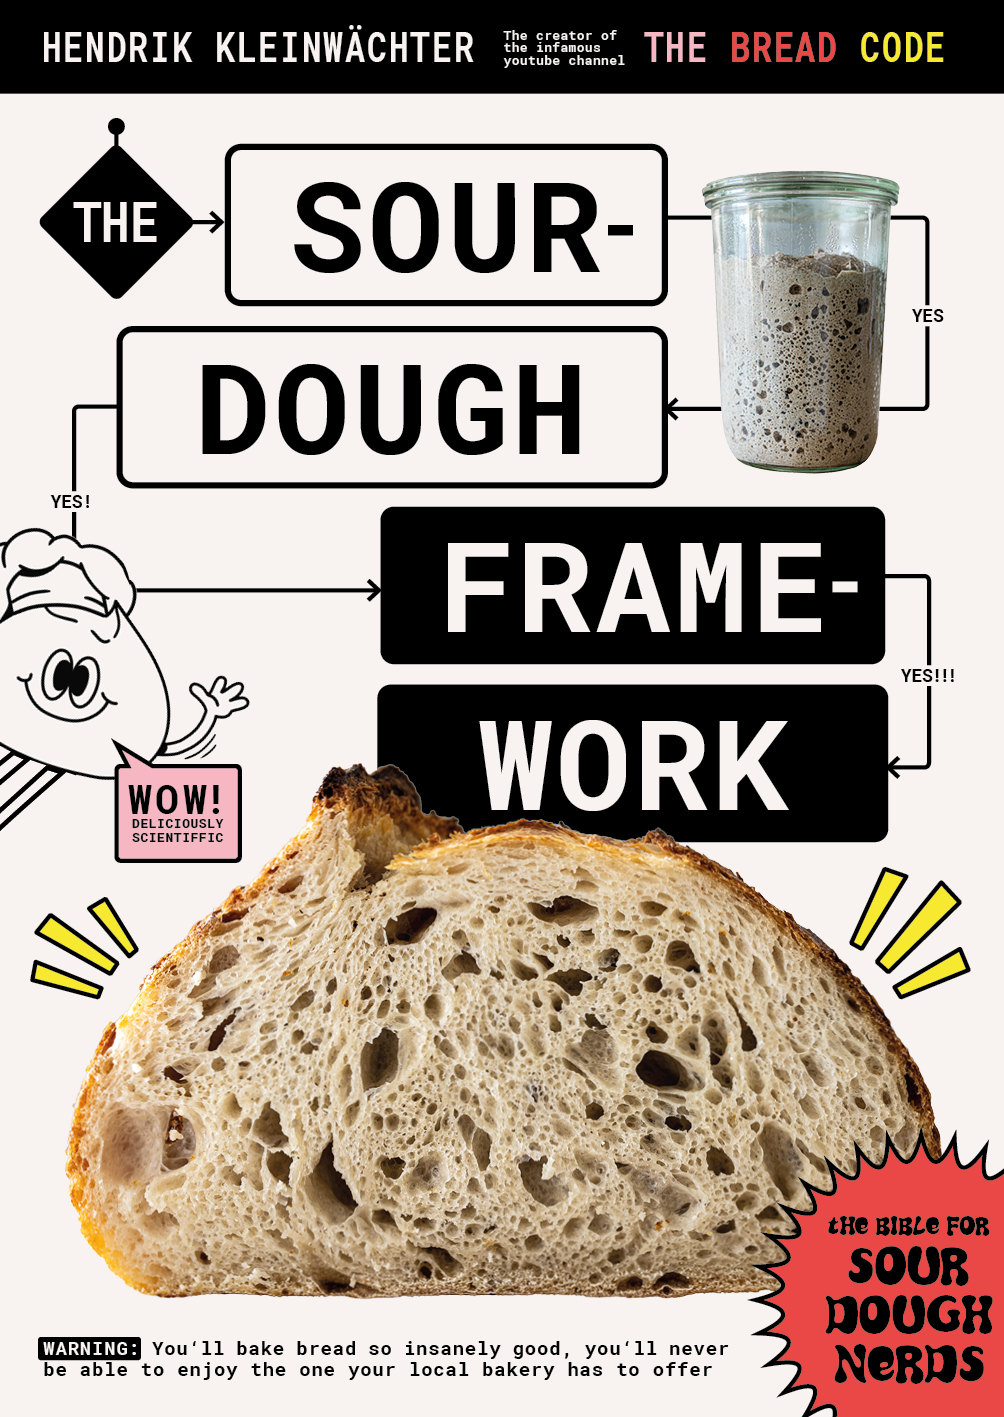
\includegraphics[width=\textwidth]{cover-page}
  Version:
  \today
\end{titlepage}


\frontmatter

\tableofcontents

\chapter{Foreword}
Hopefully one day there is going to be an awesome foreword
by another break baker!

\chapter{Preface}
If there is one food Germany is known for, it is probably bread.
There are thousands of varieties in Germany,
and making it has been an integral part of our culture.

My bread journey began during childhood. My mother, being a parent
of 3, would always use Saturdays to bake a delicious loaf for the family.
It was a white fluffy sandwich bread, and she made it within one to two hours using store-bought yeast.
Being a bit more experienced, I now realize it's
ideal to wait a little while before cutting into your bread, but back then,
we kids couldn't wait. Mom would cut for us a few slices straight from the oven, and we would
immediately proceed to pour butter or jam on each slice. Within minutes, 1 kg of
flour would be consumed. Bread became an integral part of my weekly food.

I was lucky that my parents could afford a yearly ski trip to
Alto Adige in northern Italy. In the small town called Valdaora, we
would try new restaurants every year, yet always end up in our favorite
pizza place. The pizzas there were incredible. The dough
alone was so tasty that we would order just the bread with a
bit of olive oil and salt.

Of course, my question would always be, ``Mom, can we make this at home, too, please?''
So over the years, we became friends with the owners and would receive
more and more clues as how to make the perfect pizza dough. There
are no secret ingredients inside. It's just flour, water, salt, and a bit of yeast.
How can such a simple combination of ingredients create such an incredibly delicious
pizza dough? My parents, being creatures of habit, would return every year with us,
and every year, my interest would grow. At home, Mom and I attempted to replicate
the recipe. We tried baking on a stone and on a steel. We tried adding oil to the dough and herbs
to the pizza sauce. We fell into an endless cycle of experiments. However, we never managed
to get close to the experience we had while on vacation.

Some years passed, and I eventually began my studies in the small German city of Göttingen.
For the first time, I was faced with shopping for my own bread. It was never
on my mind to actually start baking it for myself. I would just buy 
a good loaf while shopping at the supermarket. My favorite variety
was a Schwarzbrot, Korn an Korn. It’s a very dark and hearty rye bread
with added berries and sunflower seeds. Being a little naïve,
I'd never before examined the packaging of what I was buying. One day, that
changed.

I looked at the label and was shocked. The seemingly
healthy bread consisted of so many other things aside from flour and water.
The black color was not coming from the flour, but from caramelized sugar.
The packaging stated it was a sourdough bread, but then why was there additional yeast?
I thought that if it was really sourdough, it shouldn't require additional yeast, and I
soon realized that something was wrong with the bread I was buying.
I proceeded to check the other supermarket breads, only to discover that they, too,
contained ingredients I'd never heard of. That was the day I lost trust
in supermarket bread.

At home, I decided to research the proper way to make bread, and much to my surprise,
I learned that the recipes for making pizza and bread were actually quite similar, yet
there were also differences. For example, some recipes would call for fresh yeast, while
others would call for dry. Diving deep into various online forums and all their many
discussions, I became even more confused.

I tried using different flours and different brands, all in both organic and non-organic varieties.
I realized then that I knew nothing about making bread. Recipes would often contradict each other,
leaving me further confused. They seemed like little more than a collection of apparently random
steps to follow. The baking instructions and temperatures were all different, too.

Meanwhile, having completed my studies, I started work as an engineer.
We engineers are faced with many challenges. The compiler or runtime is
always screaming at you with errors, and it's your job to figure out how to fix them.
It can take hours, sometimes days, just to fix a simple problem. If you want
to become a software engineer, you have to develop a certain ``never-give-up'' attitude.

When writing code, software engineers often need to use a set of pre-made routines. These routines have been
written by other engineers and can then be used to ship code faster.
This pre-written code is commonly known as {\it a framework}. In many cases,
these frameworks are not built by a single person but by engineers from all around the world,
each of whom can help by improving and changing the source code. Frameworks have made many successful
businesses possible.

In most cases, frameworks do exactly what they claim they do. However,
sometimes you are faced with issues you don't understand. In 99.95 percent
of all software bugs, the developer is the issue. Sometimes, however, the framework has a
bug. That is when the developer must dig deeper to see the 'what' and the 'why' behind what
the framework is doing. You will need to read other engineer's source code, and you will be forced
to understand {\it why} things are happening.

Being unhappy with what I was baking, my engineering mindset took over, and I had
to do my own deep dive to understand what was going on. Much to my surprise, however,
none of the recipes I'd encountered would tell me {\it why} I should use amount X
of water and amount Y of flour, or {\it why} exactly I should use fresh yeast over dry yeast. Why
should I slap my dough while kneading it on the counter? Why is a standmixer
better than kneading by hand?  Why should I let the dough sit for this long?
Why is steaming the dough during baking important? Do I really need to
get myself an expensive Dutch oven to bake bread?

The problem compounded when I started reading about sourdough. It all sounded like black
magic. Why were some sourdoughs made from fruits, while others were made from flour?
Why should one recipe use wheat while another used rye or spelt? How often should the
sourdough be fed? The questions I had then could have filled 20 pages. I was confused,
but I became even more determined to learn how decent bread should be made at home.

The feedback I received from friends helped me to improve with each
iteration of homemade bread. Compared to coding, where you sometimes have to wait months
for this feedback, bread making is much more direct. Plus, you can eat your successes
(and failures!) And, much to my surprise, even those failures started tasting better than
most store-bought breads. Eating a homemade bread that takes you hours to make allows you
to develop a different relationship with your food, and baking bread from scratch with my
bare hands was a welcome change after hours of working on the computer.

I continued learning about the process of fermentation and various techniques of bread making.
I approached the topic of sourdough in a manner similar to software, and after years of
researching and documenting my progress, I decided it was time to share that progress with the
world.

When working on open source projects, it is important to see their history and how the source
code changes over time. This way, you can easily jump back to previous versions. This was
the perfect tool for documenting my recipes, because they, too, would change with each
subsequent iteration. Much to my surprise, my open source work on sourdough was appreciated
by other engineers, and the project became popular on the website GitHub, originally built to
share open source software.

Now, when baking great bread, you also need to learn certain techniques. I figured it would be
easier to share these techniques in video form. Thus, my YouTube channel was born. I chose
the name {\it The Bread Code} to capture my engineering-oriented approach to bread. It took some
time to get right, but after choosing more engaging thumbnails and titles for
the videos I made, the channel started gaining viewers.

Now, three years later, I dedicate two days each week to follow my bread baking passion, while
the other three days I continue to work as a software engineer, writing code on a day-to-day
basis.

My bread days fill me with both joy and passion. To me, there is nothing better than seeing
how many people have made amazing bread thanks to my tips and explanations. The community has
continued to grow, spawning many interesting discussions and ideas surrounding the topic of
bread making. There is always something new to learn, and I feel that even now I am just barely
scratching the surface with what I know and teach. Would you ever have imagined that fruit
flies are like bees and are part of the wild yeast's success story? I made a video where
I tried to cultivate wild yeast spores coming from fruit flies in order
to bake bread. It worked; the bread turned out amazingly well and even tasted good! These kinds of
experiments spark my natural interest. Conducting them and seeing how other people share in my
interest makes me incredibly happy.

The problem with running a YouTube channel is that all the information
you see is filtered and then provided to you through an algorithm. I am concerned
with how algorithms are shaping modern information, because they tend to
put users into certain categories where they will then only see news related to
those same fixed categories. A key metric determining visibility of your channel is how many
people have clicked on a video after it's been shown, and the content you create
is not even shown to every subscriber of your channel. If the algorithm determines the video
is not engaging enough, your content starts to decay in YouTube's nirvana. Even if your video
goes viral, the algorithm will stop showing it once engagement rates with new users goes down,
and older videos fade over time as the decay punishment factor increases. I know, because
I have developed similar algorithms myself as a software engineer.

I've since decided to take some time off from the algorithm cycle to work on something more
long term and meaningful. My mission has always been to share my knowledge with as many people
in the world as possible. That's also why my content has been provided in English rather than
German. After discussions with members of the community, I figured that writing a book could
help me achieve that goal. Most of the books that exist today are collections of recipes. My
idea, however, is to provide you with a deeper foundation of knowledge that you can use to
follow other recipes.

In software terms, this would be a {\it bread framework}.

It is my goal for this book to help everyone facing issues with flour, fermentation, baking,
and more. It should provide a detailed understanding as to why certain steps are necessary
and how to adapt them when things go wrong while making bread.

It is my desire for this knowledge to be accessible to everyone around the world, regardless
of budget, and as such, I do not want to charge for the book. That's why I've decided to make
it open source and have asked the community to support my work financially via my ko-fi page
(https://ko-fi.com/thebreadcode). The community's feedback has been amazing so far, and
I've already raised much more money than initially expected.

The first version of the book will only be available digitally---this way, everyone can read
it---though there might also be a hardcover version in the future, depending on how well received
and appreciated it is by bakers around the world. The hardcover version will, of course, cost a
bit of money, but the digital version will remain free.

In this book, I will try to be as scientific as possible. I in no way claim, however, that
it will itself be a work of science. I have conducted several experiments that I will write
about here, but to truly call this science, you would probably need to repeat the same experiment
a thousand times in a lab environment, which I have not done. I will do my best, however, to provide
scientific references where possible and to clearly distinguish between facts and personal opinion.

I hope you have fun reading this and that you learn more about the fascinating world of bread
making, and it is my sincere wish that this work provides you with the solid toolchain that I wish
I'd had access to when starting my own journey with bread.

Thank you.
Hendrik


\chapter{Acknowledgements}
This book would not have been possible without your help.

With all your donations I have been able to take time off from my job and
focus on this project.

Furthermore many of you have contributed and improved the
instructions, fixed spelling mistakes and/or provided
feedback on the content. Each of you has made this book
better.

By providing this book free of charge,
we can enable more people around the world to bake delicious sourdough
bread at home.

Thank you very much for your support!\\

\begin{filecontents}{supporters.csv}
  \end{filecontents}

  {Big shout-out to all the initial supporters who helped launching this project:}

  \pgfplotstableset{
  begin table=\begin{longtable},
  end table=\end{longtable},
  }

  \pgfplotstabletypeset[col sep=comma,
  header=true,
  columns={Name},
  columns/Name/.style={column type=l,string type},
  every head row/.style={before row=\toprule, after row=\midrule\endhead},
  every last row/.style={after row=\bottomrule}
  ]{supporters.csv}


\mainmatter

\chapter{The history of sourdough}
\chapter{The history of sourdough}%
\label{ch:history}
\begin{quoting}
    We will start this book by briefly talking about the long history of
    sourdough bread from ancient time, and how people used similar process for
    other food like beer. The discovery of yeast and how, together with
    machine development, revolutionized bread making.  More recently
    communities formed around sourdough and home baking, trying to relearn
    lessons from the past.
\end{quoting}

The story of sourdough bread begins in prehistoric oceans. These oceans were the
birthplace of all life on Earth. To better envision the vast history of
our planet, lets create a timeline in one~year/365~days. On this scale,
January~1 signifies Earth's
formation 4.54~billion years ago. Midnight on December~31 is the present.
Each day represents roughly 12~million years. This technique simplifies the
complexity of time but also renders the extraordinary expanse of our planet's
history into a more graspable timeframe. We humans, are in fact a recent
addition to our planet, so young that we made our first appearance on
the evening of December~31.  It seems that humans managed to arrive just
in time to join the celebration at the end of the year.

On March~25, the oceans birthed the first single-celled bacteria. In these
waters, another single-celled life form, \emph{archaea}, also thrived. These
organisms inhabit extreme environments, from boiling vents to icy waters.

\begin{figure}[!htb]
  \centering
  \begin{tikzpicture}
  % Draw horizontal line
  \draw[line width=1pt] (0,0) -- (\textwidth,0);

  % Define the width of each segment
  \pgfmathsetlengthmacro{\segmentwidth}{\textwidth/12}

  % Draw lines for the events, higher up so that they don't overflow the text
  % Placing the lines has been a bit manual work of trying different values
  % Maritime bacteria.

  \draw[line width=1pt] (2.8*\segmentwidth,1) -- (2.8*\segmentwidth,0.2);
  % Eukaryotes
  \draw[line width=1pt] (5.8*\segmentwidth,1.5) -- (5.8*\segmentwidth,0.2);
  % First bacteria on land
  \draw[line width=1pt] (9.1*\segmentwidth,-1.25) -- (9.1*\segmentwidth,-0.2);
  % Maritime fungi ancestors
  \draw[line width=1pt] (9.5*\segmentwidth,-2) -- (9.5*\segmentwidth,-0.2);
  % Fungi on land
  \draw[line width=1pt] (10.8*\segmentwidth,-2.75) -- (10.8*\segmentwidth,-0.2);
  % Yeasts on land
  \draw[line width=1pt] (11.1*\segmentwidth,-3.0) -- (11.1*\segmentwidth,-0.2);
  % First dinosaurs
  \draw[line width=1pt] (11.4*\segmentwidth,1) -- (11.4*\segmentwidth,0.2);
  % Dinosaur extinction
  \draw[line width=1pt] (11.9*\segmentwidth,1.5) -- (11.9*\segmentwidth,0.2);

  % Special lines for december events since they are so close togehter
  \draw[line width=1pt] (12.0*\segmentwidth,3.0) -- (12.0*\segmentwidth,0.2);  % Main branch
  \draw[line width=1pt] (12.0*\segmentwidth,3.0) -- (11.75*\segmentwidth,2.5); % Branch to first humans
  \draw[line width=1pt] (12.0*\segmentwidth,3.0) -- (11.75*\segmentwidth,3.0); % Branch to Jordan
  \draw[line width=1pt] (12.0*\segmentwidth,3.0) -- (11.75*\segmentwidth,3.5); % Branch to Pasteur

  % Draw months and month separators
  \foreach \i/\month in {0/Jan, 1/Feb, 2/Mar, 3/Apr, 4/May, 5/Jun, 6/Jul, 7/Aug, 8/Sep, 9/Oct, 10/Nov, 11/Dec} {
      % Separators
      \draw[line width=1pt] (\i*\segmentwidth,0.1) -- (\i*\segmentwidth,-0.1);
      % Month names
      \node[timeline_event, below] at ({(\i+0.5)*\segmentwidth},-0.1) {\month};
  }
  \draw[line width=1pt] (\textwidth,0.1) -- (\textwidth,-0.1);

  % Place events on the timeline with dates using the timeline_event style
  % As a calculation I used (4.54 billion years / 12 months = 0.3785 billion years/month.
  \node[timeline_event, above] at (2.0*\segmentwidth,1) {Mar 25 - First maritime bacteria and archae};
  \node[timeline_event, above] at (4.50*\segmentwidth,1.5) {June 25 - First organisms with nuklei (eukaryotes)};
  \node[timeline_event, above] at (7.8*\segmentwidth,-1.5) {Oct 4 - First bacteria on land};
  \node[timeline_event, above] at (8.0*\segmentwidth,-2.25) {Oct 15 - First maritime ancestors of fungi};
  \node[timeline_event, above] at (9.7*\segmentwidth,-2.75) {Nov 24 - Fungi on land};
  \node[timeline_event, above] at (10.5*\segmentwidth,-3.25) {Dec 3 - Yeasts on land};
  \node[timeline_event, above] at (10.25*\segmentwidth,1) {Dec 14 - First dinosaurs};
  \node[timeline_event, above] at (10.33*\segmentwidth,1.5) {Dec 29 - Dinosaurs go extinct};
  \node[timeline_event, above, anchor=east, align=right] at (11.75*\segmentwidth,2.5) {Dec 31 - First humans};
  \node[timeline_event, above, anchor=east, align=right] at (11.75*\segmentwidth,3.0) {Dec 31 - Sourdough in Jordan (23:59:55)};
  \node[timeline_event, above, anchor=east, align=right] at (11.75*\segmentwidth,3.5) {Dec 31 - Louis Pasteur isolated yeast (23:59:59)};

\end{tikzpicture}

  \caption[Sourdough microbiology timeline]{Timeline of significant events
    starting from the first day of Earth's existence,
    divided into months, and extending to the present day,
    marked at midnight. This visualization shows the pivotal steps
    of life and sourdough on earth.}%
  \label{fig:planet-timeline}
\end{figure}

Whoever comes first, bacteria or archaea, remains debated. For three
months (or approximately 1.1~billion years), these life forms dominated
the oceans. Then, on June~25 in a highly unlikely event, an archaeon consumed a bacterium.
Instead of digesting it, they formed a symbiotic relationship. This led to the
first nucleated organisms, marking an evolutionary milestone. This event lead
to the development of plants, fungi and also ultimately humans.

Life stayed aquatic for another three months.
On October~4, bacteria first colonized land. By October~15, the
first aquatic fungi appeared. They adapted and, by November~24, had colonized
land.

By December~3, yeasts emerged on land. This laid groundwork for bread-making.
Jump 140~million years to December~14, and dinosaurs arose. Just a couple
of days after their appearance on December~17 the super continent Pangea
started to rift apart, reshaping the continents into their current form.
The dinosaurs reigned until December~29 when they faced extinction.
Another 25~million years later, or our timeline's 2~days after the dinosaur
extinction, humans appeared.

A few hours later after the arrival of humans, a more subtle culinary
revolution was unfolding. By \num{12000}~BC, just 5~seconds before our
metaphorical midnight, the first sourdough breads were being baked in ancient
Jordan. A blink of an eye later, or 4~seconds in our time compression,
Pasteur's groundbreaking work with yeasts set the stage for modern
bread-making. From the moment this book began to take shape to your current
reading, only milliseconds have ticked by~\cite{Yong+2017}.

Now delving deeper into the realm of sourdough, it can likely be traced to aforementioned
Ancient Jordan~\cite{jordan+bread}. Looking at the earth's timeline sourdough
bread can be considered a very recent invention.

\begin{figure}[!htb]
  \centering
  \begin{tikzpicture}
  % Draw horizontal line
  \draw[line width=1pt] (0,0) -- (\textwidth,0);

  % Define the width of each segment
  \pgfmathsetlengthmacro{\segmentwidth}{\textwidth/12}

  % Lines for periods
  \draw[stealth-stealth, line width=1pt] (0,-4.2)
    -- node[midway, timeline_timespan] {Historic breadmaking} ({\segmentwidth * 7.8},-4.2);
  \draw[stealth-stealth, line width=1pt] ({\segmentwidth * 7.8},-4.2)
    -- node[midway, timeline_timespan] {Modern bread} ({\segmentwidth * 12},-4.2);

  % Regularly placed events, not in chronological order
  % since should be placed on top of others on the timeline
  \draw[line width=1pt] ({\segmentwidth*3},1.5) -- ({\segmentwidth*3},0.3)
    node[at start, above, timeline_event] {6000 BC: First beer in Egypt};
  \draw[line width=1pt] ({\segmentwidth*5.95},2.5) -- ({\segmentwidth*5.95},0.3)
    node[at start, above, timeline_event] {70 BC:~First water mill};

  \draw[line width=1pt] ({\segmentwidth*10.50},2.5) -- ({\segmentwidth*10.50},0.3);
  \node[timeline_event, above, anchor=east] at ({\segmentwidth*12.50},2.5) {1950:~Modern Wheat};

  \draw[line width=1pt] ({\segmentwidth*11.20},-3.25) -- ({\segmentwidth*11.20},-0.3);
  \node[timeline_event, above, anchor=east] at ({\segmentwidth*12.20},-3.5) {2020~COVID-19 Pandemic};

    \draw[line width=1pt] ({\segmentwidth*9.60},1.5) -- ({\segmentwidth*9.60},0.3)
    node[at start, above, timeline_event] {1868:~Commercial yeast};
  \draw[line width=1pt] ({\segmentwidth*7.8},0.75) -- ({\segmentwidth*7.8},0.3)
    node[at start, above, timeline_event] {1680:~Discovery of microorganisms};
  \draw[line width=1pt] ({\segmentwidth*9.80},-2.5) -- ({\segmentwidth*9.80},-0.3)
    node[at start, below, timeline_event] {1885:~Electrical mixer};
  \draw[line width=1pt] ({\segmentwidth*9.57},-1.75) -- ({\segmentwidth*9.57},-0.3)
    node[at start, below, timeline_event] {1857:~Isolated Yeast};
  \draw[line width=1pt] ({\segmentwidth*8.80},-1.25) -- ({\segmentwidth*8.80},-0.3)
    node[at start, above, timeline_event] {1785:~Steam mill};

  % Lines to events
  % Cultivation of Einkorn
  \draw[line width=1pt] (0,1) -- (0,0.3);
  \draw[line width=1pt] (0,1) -- (0.25,1);
  \node[timeline_event, above, anchor=west] at (0.25,1) {12000 BC:~Cultivation of Einkorn};

  % Sourdough in Jordan
  \draw[line width=1pt] (0,-1) -- (0,-0.3);
  \draw[line width=1pt] (0,-1) -- (0.25,-1);
  \node[timeline_event, above, anchor=west] at (0.25,-1) {12000 BC:~Sourdough in Jordan};
  % Events

  % Indicators for period
  % Draw months and month separators
  \foreach \i/\month in {0/12000, 1/10000, 2/8000, 3/6000, 4/4000, 5/2000,
  6/0, 7/1600, 8/1700, 9/1800, 10/1900, 11/2000, 12/2100} {
      % Separators
      \draw[line width=1pt] (\i*\segmentwidth,0.1) -- (\i*\segmentwidth,-0.1);
      % Events for timeline
      \node[timeline_event, below] at ({(\i)*\segmentwidth},-0.1) {\month};
  }
\end{tikzpicture}

  \caption[Sourdough history timeline]{Timeline of significant discoveries and
  events leading to modern sourdough bread.}%
  \label{fig:sourdough-timeline}
\end{figure}

The exact origins of fermented
bread are, however, unknown. One of the most ancient preserved
sourdough breads has been excavated in Switzerland~\cite{switzerland+bread}.

\begin{figure}[ht]
  \centering
  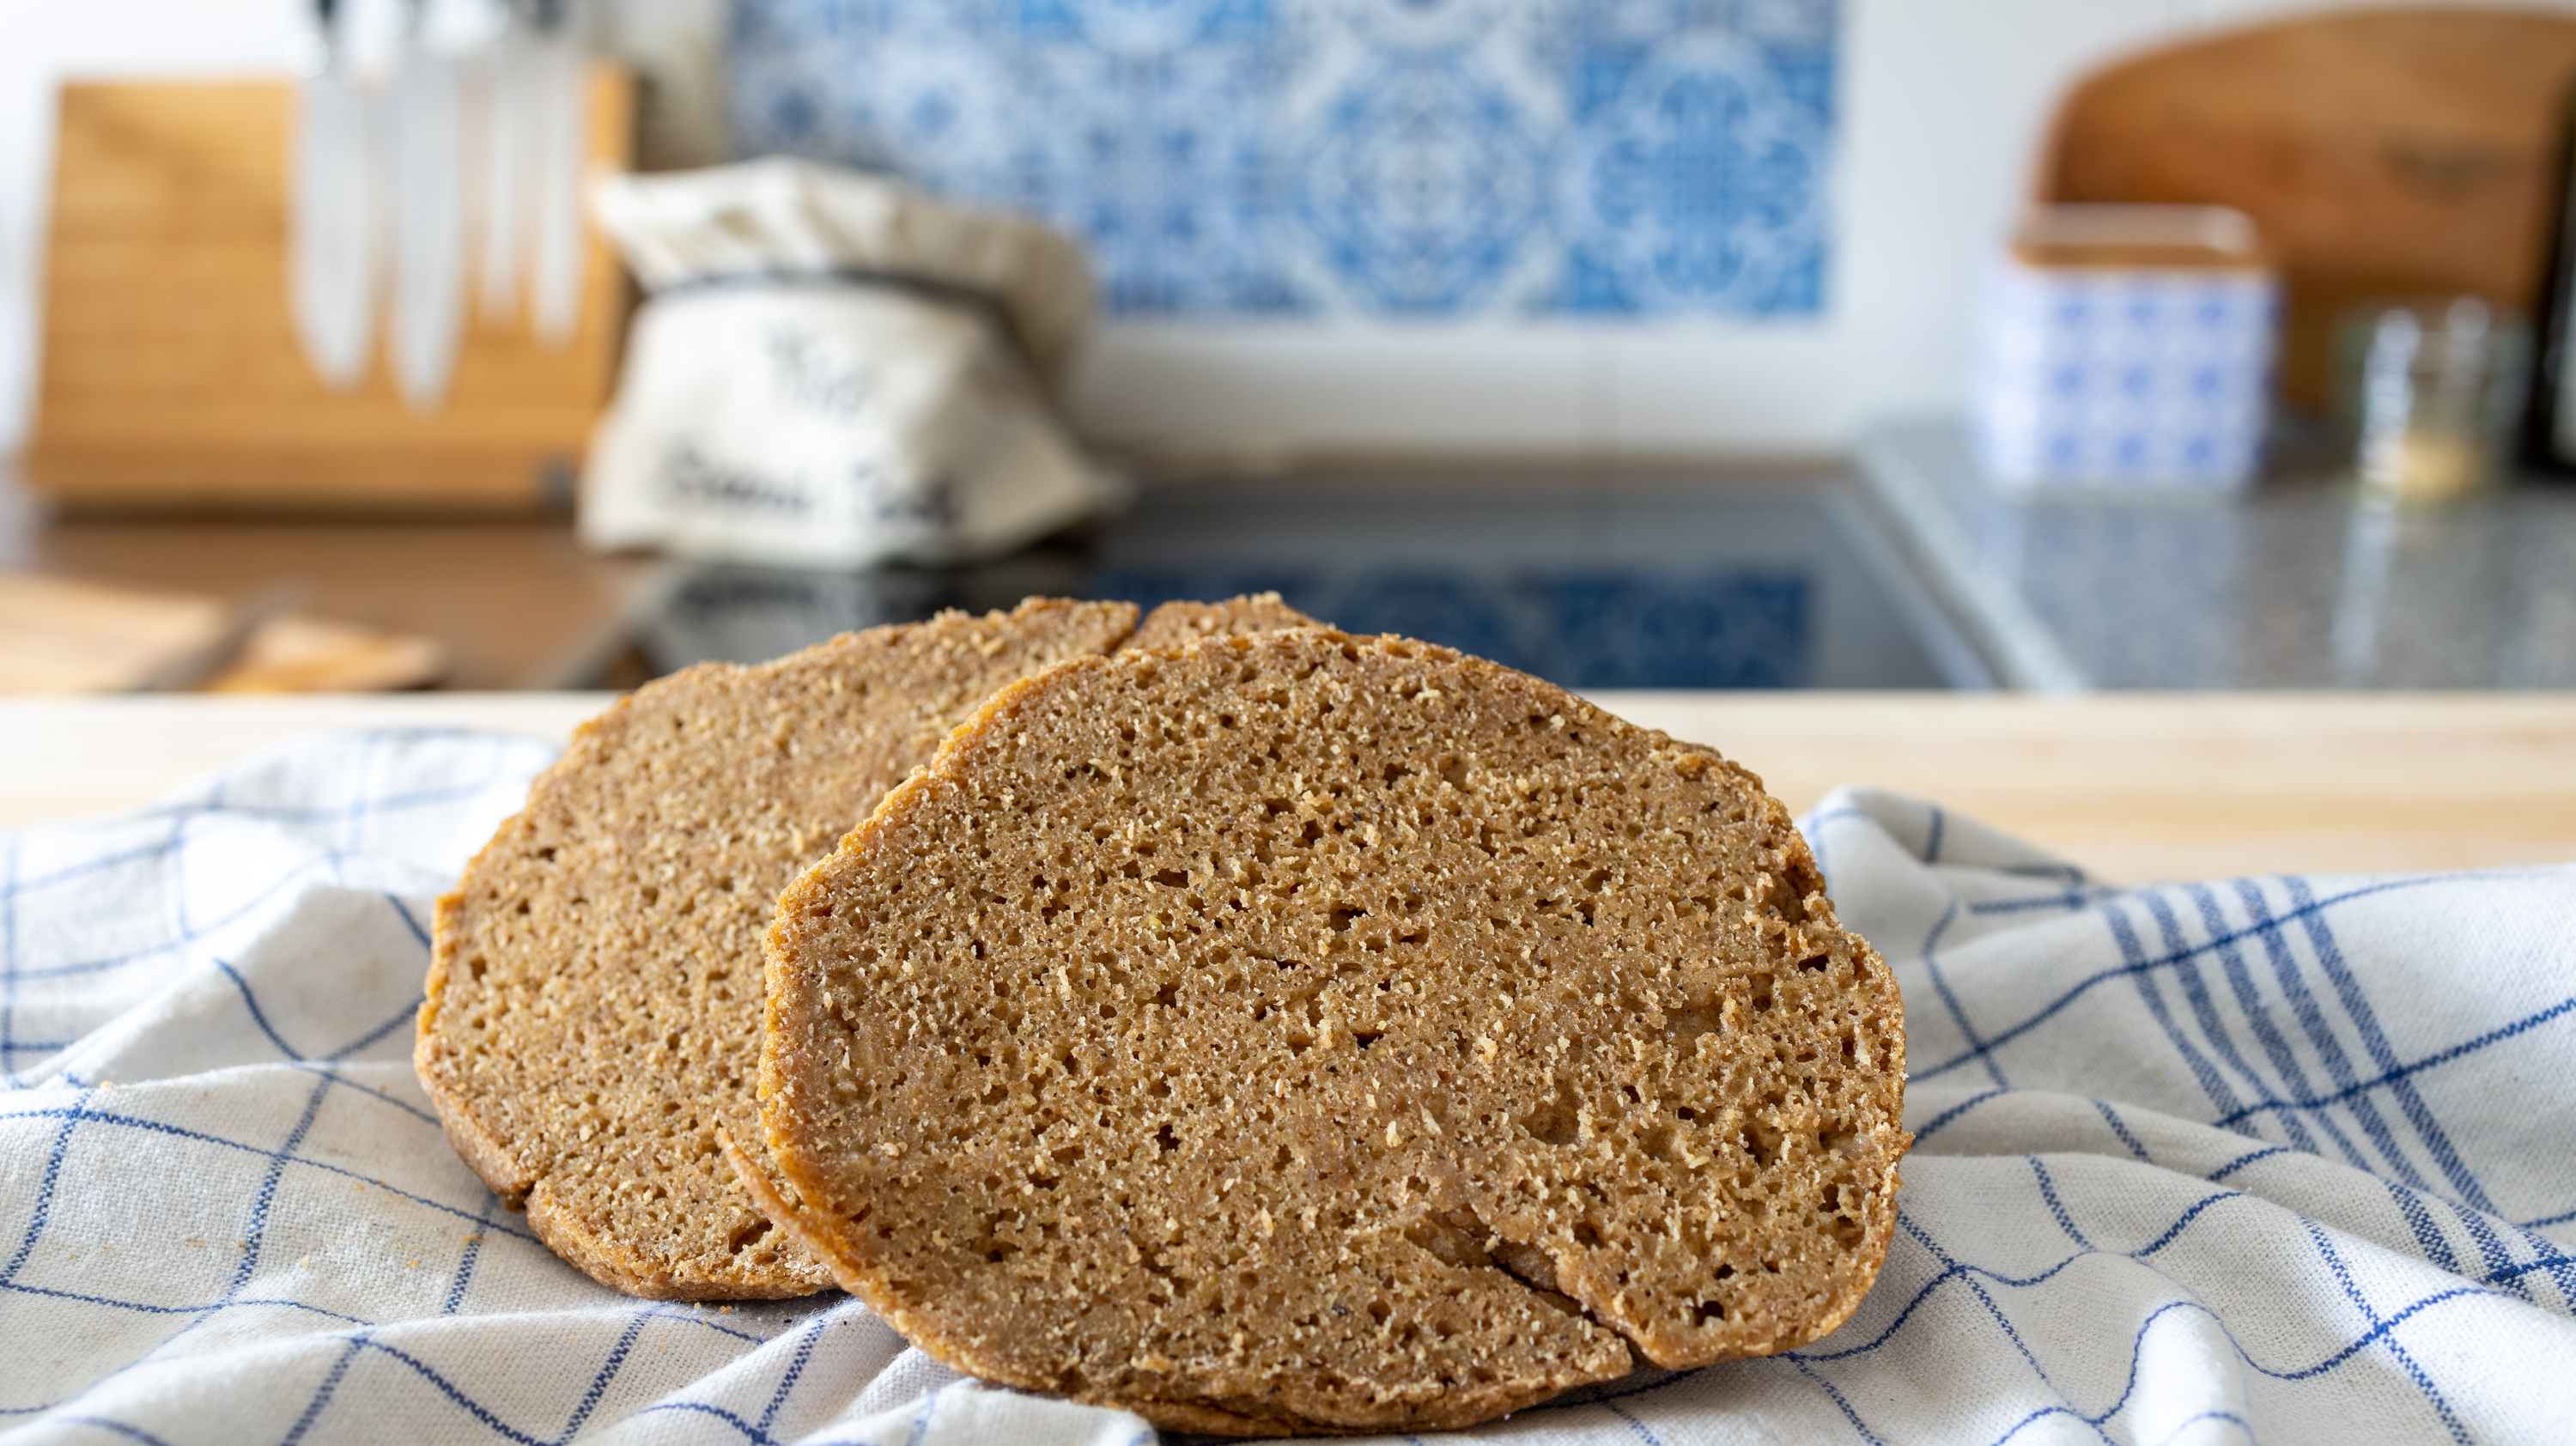
\includegraphics[width=\textwidth]{einkorn-crumb}
  \caption[Ancient Einkorn flatbread]{An ancient Einkorn flatbread. Note the
      dense crumb structure.}%
  \label{fig:einkorn-crumb}
\end{figure}

Another popular story is that a lady in Egypt was making
a bread dough close to the Nile river. The lady forgot the
dough and at her return a few days later, she noticed that the dough had
increased in size and smelled funky. She decided to bake
the dough anyway and was rewarded with a much
lighter, softer, better tasting bread dough. From that day
on she continued to make bread this way~\cite{egyptian+bread}.

Little did the people back then know that tiny microorganisms
were the reason the bread was better. It is not clear when
they started using a bit of the dough from the previous
day for the next batch of dough. But by doing so, sourdough
bread making---as we know it today---was born: Wild yeast
in the flour and in the air, with bacteria
starting to decompose the flour-water mixture.
The yeast makes the dough fluffy,
and the bacteria primarily creates acidity. The different
microorganisms work in a symbiotic relationship. Humans
appreciated the enhanced airy structure and slight acidity
of the dough. Furthermore, the shelf life of such bread
was extended due to the increased acidity.

Quickly, similar processes were discovered when brewing beer
or making wine. A small tiny batch of the previous production
would be used for the next production. In this way, humans created
modern bread yeasts, wine yeasts, and beer yeasts~\cite{egypt+beer}.

Over time with each batch, the yeasts and bacteria
would become better at consuming whatever they were thrown at.
By feeding your sourdough starter, you are selectively breeding
microorganisms that are good at eating your flour. With
each iteration, your sourdough knows how to better ferment the flour
at hand. This is also the reason\footnote{It is crazy if you think about it.
People have been using this process despite not knowing what was going on for
thousands of years!} why more mature sourdough starters sometimes tend to
leaven doughs faster~\cite{review+of+sourdough+starters}.  The sourdough in
itself is a symbiotic relationship, but the sourdough
also adapted to humans and formed a symbiotic relationship with us.
For food and water, we are rewarded with delicious bread. In exchange,
we shelter and protect the sourdough. Spores from the starter
are spread through aerial contamination or insects like fruit flies.
This allows the sourdough starter to spread its spores even
further all around the world.

Evidence suggests early grain grinding in northern Australia around
\num{60000}~BC, notably at the Madjedbebe rock shelter in Arnhem
Land~\cite{aboriginal+grinding+stones}.  However, a more significant
advancement occurred later, as documented by the ancient Greek geographer
Strabo in \num{71}~BC\@.  Strabo's writings described the first water-powered
stone mill, known as a \emph{gristmill}. These mills advanced flour production
from a few kilograms up to several metric tons per day~\cite{history+mills}.

These early mills featured horizontal paddle wheels, eventually termed
\emph{Norse wheels} due to their prevalence in Scandinavia.  The paddle wheels
connected to a shaft, which, in turn, linked to the central runner stone for
grinding. Water flow propelled the paddle wheels, transferring the grinding
force to the stationary \emph{bed}, typically a stone of similar size and
shape. This design was straightforward, avoiding the need for gears. However,
it had a limitation: the stone's rotation speed relied on water volume and
flow rate, making it most suitable for regions with fast-flowing streams,
often found in mountainous areas~\cite{mills+scandinavia}.

In the year \num{1680}, a remarkable scientist by the name of
Antonie~van~Leeuwenhoek introduced a groundbreaking innovation that would
forever alter our understanding of the microscopic world and ultimately bread
making.  Van~Leeuwenhoek, a master of lens craftsmanship, possessed an
insatiable fascination with realms invisible to the naked eye. His pioneering
work birthed the first modern microscope.  What set Van~Leeuwenhoek apart was
the exceptional quality of his lenses, capable of magnifying tiny
microorganisms by an astounding factor of \num{270}.  Driven by an unrelenting
curiosity to unveil the unseen, he embarked on a journey of exploration. He
scrutinized flies, examined lice-infested hair, and ultimately turned his gaze
toward the tranquil waters of a small lake near Delft.

In this serene aquatic habitat, he made astonishing observations, discovering
algae and minuscule, dancing creatures hitherto hidden from human perception.
Eager to share his revelatory findings with the scientific community,
Van~Leeuwenhoek faced skepticism, as it was difficult to fathom that someone
had witnessed thousands of diminutive, dancing entities—entities so tiny that
they eluded the human eye.

Undeterred by skepticism, he continued his relentless pursuit of the unseen,
directing his lens towards a brewer's beer sludge. In this obscure medium,
Van~Leeuwenhoek made history by becoming the first human to lay eyes upon
bacteria and yeast, unraveling a previously concealed world that would
revolutionize our understanding of microbiology~\cite{Yong+2017+Leeuwen}.

At the same time brewers would start to experiment with utilizing the muddy
leftovers of the beer fermentation to start making doughs. They would notice
that the resulting bread doughs were becoming fluffy and compared
to the sourdough process would lack the acidity in the final product.
A popular example is shown in a report from \num{1875}. Eben Norton Horsford
wrote about the famous \emph{Kaiser Semmeln} (Emperor's bread rolls).
These are essentially bread rolls made with brewer's yeast instead
of the sourdough leavening agent. As the process is more expensive,
bread rolls like these were ultimately consumed by the noble people
in Vienna~\cite{vienna+breadrolls}.

Industrialization of the grist milling process, starting in the late
18\textsuperscript{th}~century with Oliver Evans (\num{1785}) and his mill
designs for continuous hands-off flour production~\cite{evans+mill}, and
evolving to steam-powered mills, made possible significant advancements in
bread production.

\begin{figure}[ht]
  \centering
  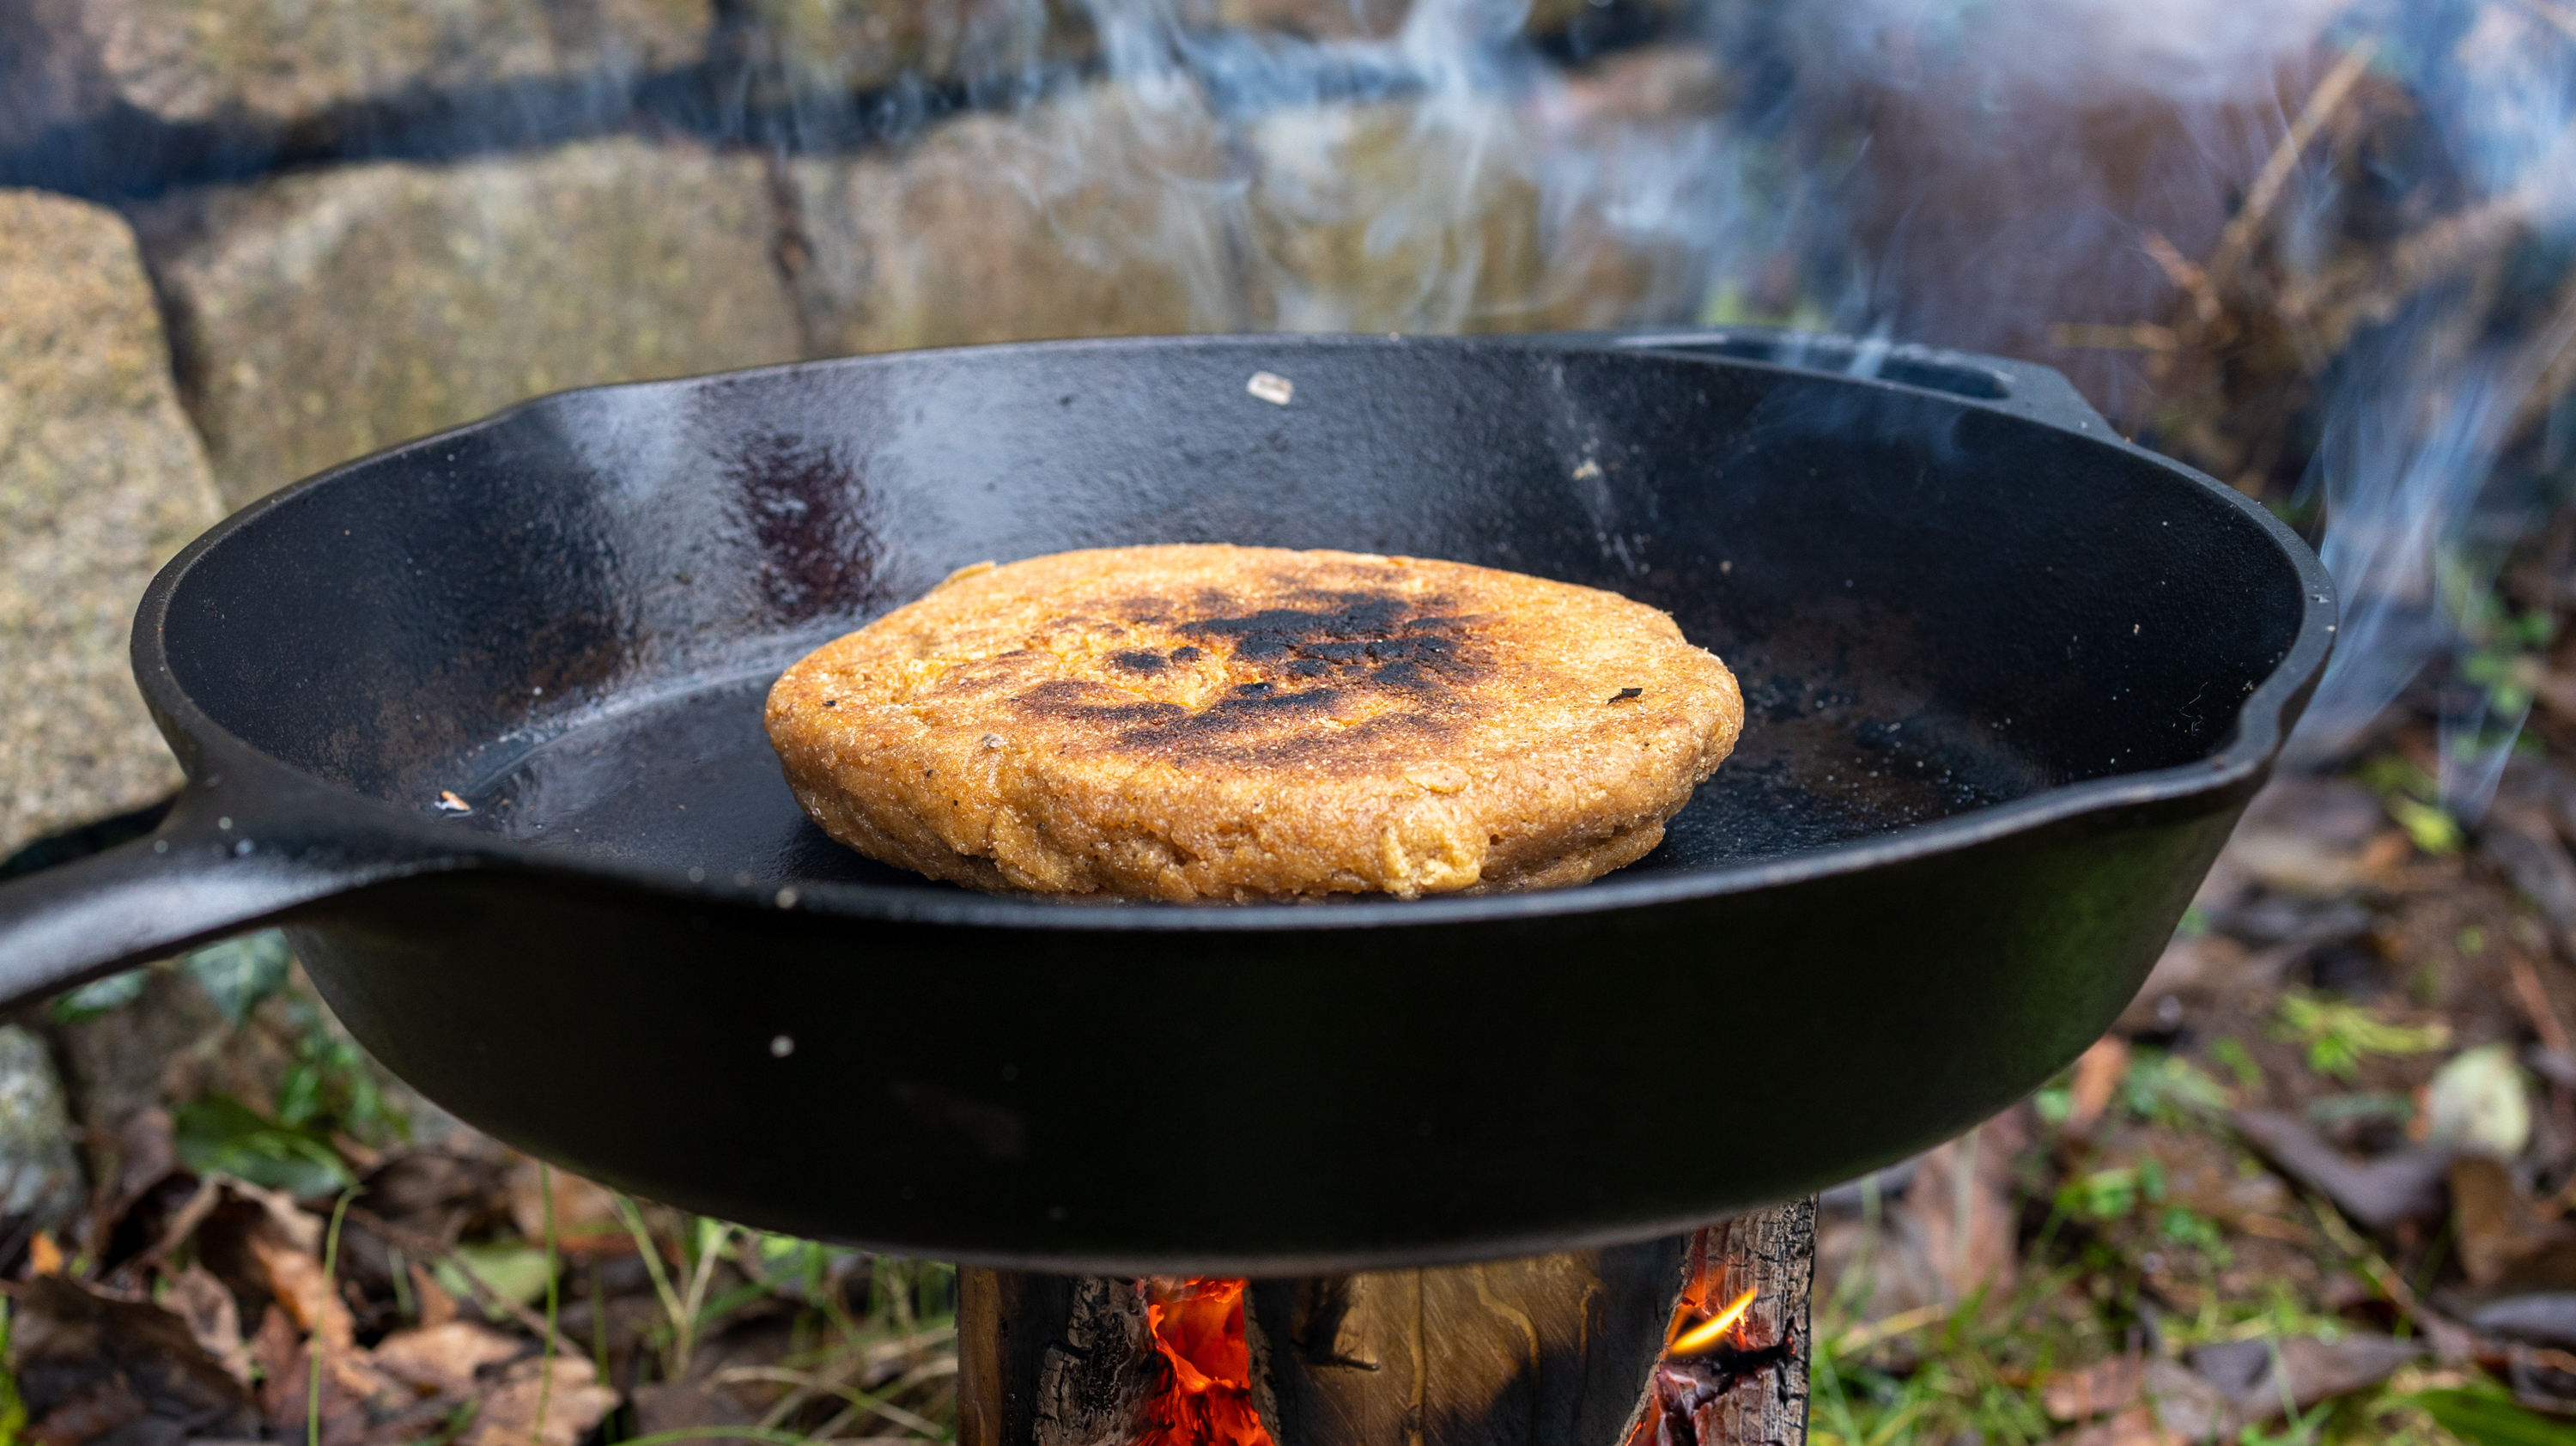
\includegraphics[width=\textwidth]{sourdough-stove}
  \caption{A bread made over the stove without an oven.}%
  \label{fig:sourdough-stove}
\end{figure}

The biggest advancement of industrial bread making happened in \num{1857}.
The French microbiologist Louis Pasteur discovered the process of alcoholic
fermentation. He would prove that yeast microorganisms are the reason for
alcoholic fermentation and not other chemical catalysts. He continued with his
research and was the first person to isolate and grow pure yeast strains.
Soon later in \num{1868} the Fleischmann brothers Charles and Maximilian were
the first to patent pure yeast strains for bread making. The yeasts offered
were isolated from batches of sourdough. By \num{1879} the machinery was built
to multiply the yeast in large centrifuges~\cite{fleischmann+history}.  The
pure yeast would prove to be excellent and turbocharged at leavening bread
doughs. What would previously take 10~hours to leaven a bread dough could now
be done within 1~hour.  The process became much more efficient. What
ultimately made making large batches of dough possible, was the invention of
the electrical kneader.  Rufus Eastman, an American inventor, is often
credited with an important advancement in mixer technology. In \num{1885}, he
received a patent for an electric mixer with a mechanical hand-crank
mechanism.  This device was not as advanced or as widely adopted as later
electric mixers, but it was an early attempt to mechanize mixing and kneading
processes in the kitchen using electricity.  Eastman's invention represented
an important step in the development of electric mixers, but it wasn't as
sophisticated or popular as later models like the KitchenAid mixer. The
KitchenAid mixer, introduced in \num{1919}, is often recognized as one of the
first widely successful electric mixers and played a significant role in
revolutionizing kitchen appliances for home
cooks~\cite{first+mixer}~\cite{kitchenaid+history}.

During World~War~II the first packaged dry yeast was developed. This would
ultimately allow bakeries and home bakers to make bread much faster and more
consistently. Thanks to pure yeast, building industrial bread making machines
was now possible. Provided you maintain the same temperature, same flour and
yeast strains fermentation became precisely reproducible. This ultimately lead
to the development of giga bakeries and flour blenders. The bakeries demanded
the same flour from year to year to bake bread in their machines.  For this
reason, none of the supermarket flour you buy today is single origin.  It is
always blended to achieve exactly the same product throughout the years.

Modern wheat, specifically the high-yielding and disease-resistant varieties
commonly grown today, began to be developed in the mid-20\textsuperscript{th}
century. This period is often referred to as the \emph{Green Revolution.}

One of the key figures in this development was American scientist Norman
Borlaug, who is credited with breeding high-yield wheat varieties,
particularly dwarf wheat varieties, that were resistant to diseases and could
thrive in various environmental conditions. His work, which started in the
1940s and continued through the \num{1960}s, played a crucial role in
increasing wheat production worldwide and alleviating food
shortages~\cite{green+revolution}.

As fermentation
times sped up, the taste of the final bread would deteriorate.
The sprouting process induced by certain enzymes is essential
to developing a fluffier texture and better tasting crust. This
can't be indefinitely sped up. Soon bakeries would start
to introduce additional enzymes to achieve similar properties
to sourdough bread in yeast-based doughs. Sourdough almost completely
vanished from the surface of the Earth. Only a handful
of true nerds would continue making bread with sourdough.

Suddenly people started to talk more often about celiac disease
and the role of gluten. The disease isn't new; it has first
been described in \num{250}~AD~\cite{coeliac+disease}. People
would note how modern bread has much more gluten compared
to ancient bread. The bread in ancient times probably was much flatter.
The grains over time have been bred more and more towards containing a higher
amount of gluten. Gluten is a protein that gives modern
bread its typical soft fluffy crumb structure. The
gluten proteins bind together once activated with water.
Throughout the course of the fermentation, \ch{CO2} is trapped
in this protein matrix. The tiny created chambers expand
during the baking process. As the dough gelatinizes while
being heated, the structure is fortified. This makes the bread appear
soft and fluffy when tasting it. Similar to drinking raw cow's milk,
your immune system might react to the consumed proteins.
There is gluten intolerance
and celiac disease. When people say they don't handle
gluten well, it's mostly a gluten intolerance they describe.
Some people describe similar issues when consuming
too much lactose. If you eat a long-fermented cheese
however, most of the lactose has been fermented by
the tiny microorganisms. People would investigate and
note how sourdough bread can typically be handled better
compared to plain, fast-made factory bread. The
reason for this is that enzymes take time to work the dough.
Gluten is a storage protein of flour. Once
sprouting is activated by adding water, the protease
enzyme starts to convert the gluten into tinier amino acids
that are required for sprouting. Over time you are effectively
losing gluten as it's naturally broken down. Furthermore,
traditionally lactic acid bacteria would start to decompose
the flour-water mix. Almost everything is recycled in nature.
Part of their diet is to consume the proteins in the dough.
Modern bread is faster and no longer has lactic acid bacteria.
Both factors together mean that you are consuming products
with a much higher gluten value compared to ancient times
when natural fermentation was used~\cite{raffaella+di+cagno}.

During the California Gold Rush, French bakers brought the sourdough
culture to Northern America. A popular bread became the
San Francisco sourdough. It's characterized by its unique
tang (which was previously common for every bread). It
however remained more of a niche food while industrial bread
was on the rise. What really expedited
the comeback of sourdough was the \num{2020} COVID-19 pandemic.
Flour and yeast became scarce in the supermarkets. While
flour returned yeast couldn't be found. People started
to look for alternatives and rediscovered the ancient
way of making sourdough bread. Soon many realized
that making sourdough bread is more complex than modern
yeast-based bread. You need to maintain a sourdough starter
and have it in ideal shape to properly ferment your dough.
Furthermore, compared to a yeast-based dough, you can't just
punch the dough down and let the fermentation continue.
You can overferment your dough, resulting in a sticky
dough mess. This complexity led to many bakers looking
for help and many thriving communities formed around
the topic of homemade bread.

When interviewing Karl de~Smedt (owner of the Sourdough
Library) he said something that changed my way of thinking
about bread: ``The future of
modern bread is in the past~\cite{interview+karl+de+smedt}.''


\chapter{How sourdough works}
In this chapter, we will cover the basics of how sourdough ferments.
First, we will look at the enzymatic reactions that take place
in your flour the moment you add water, triggering the fermentation
process. Then, in order to better understand this process, we will
learn more about the yeast and bacterial microorganisms involved.

\begin{figure}[!htb]
  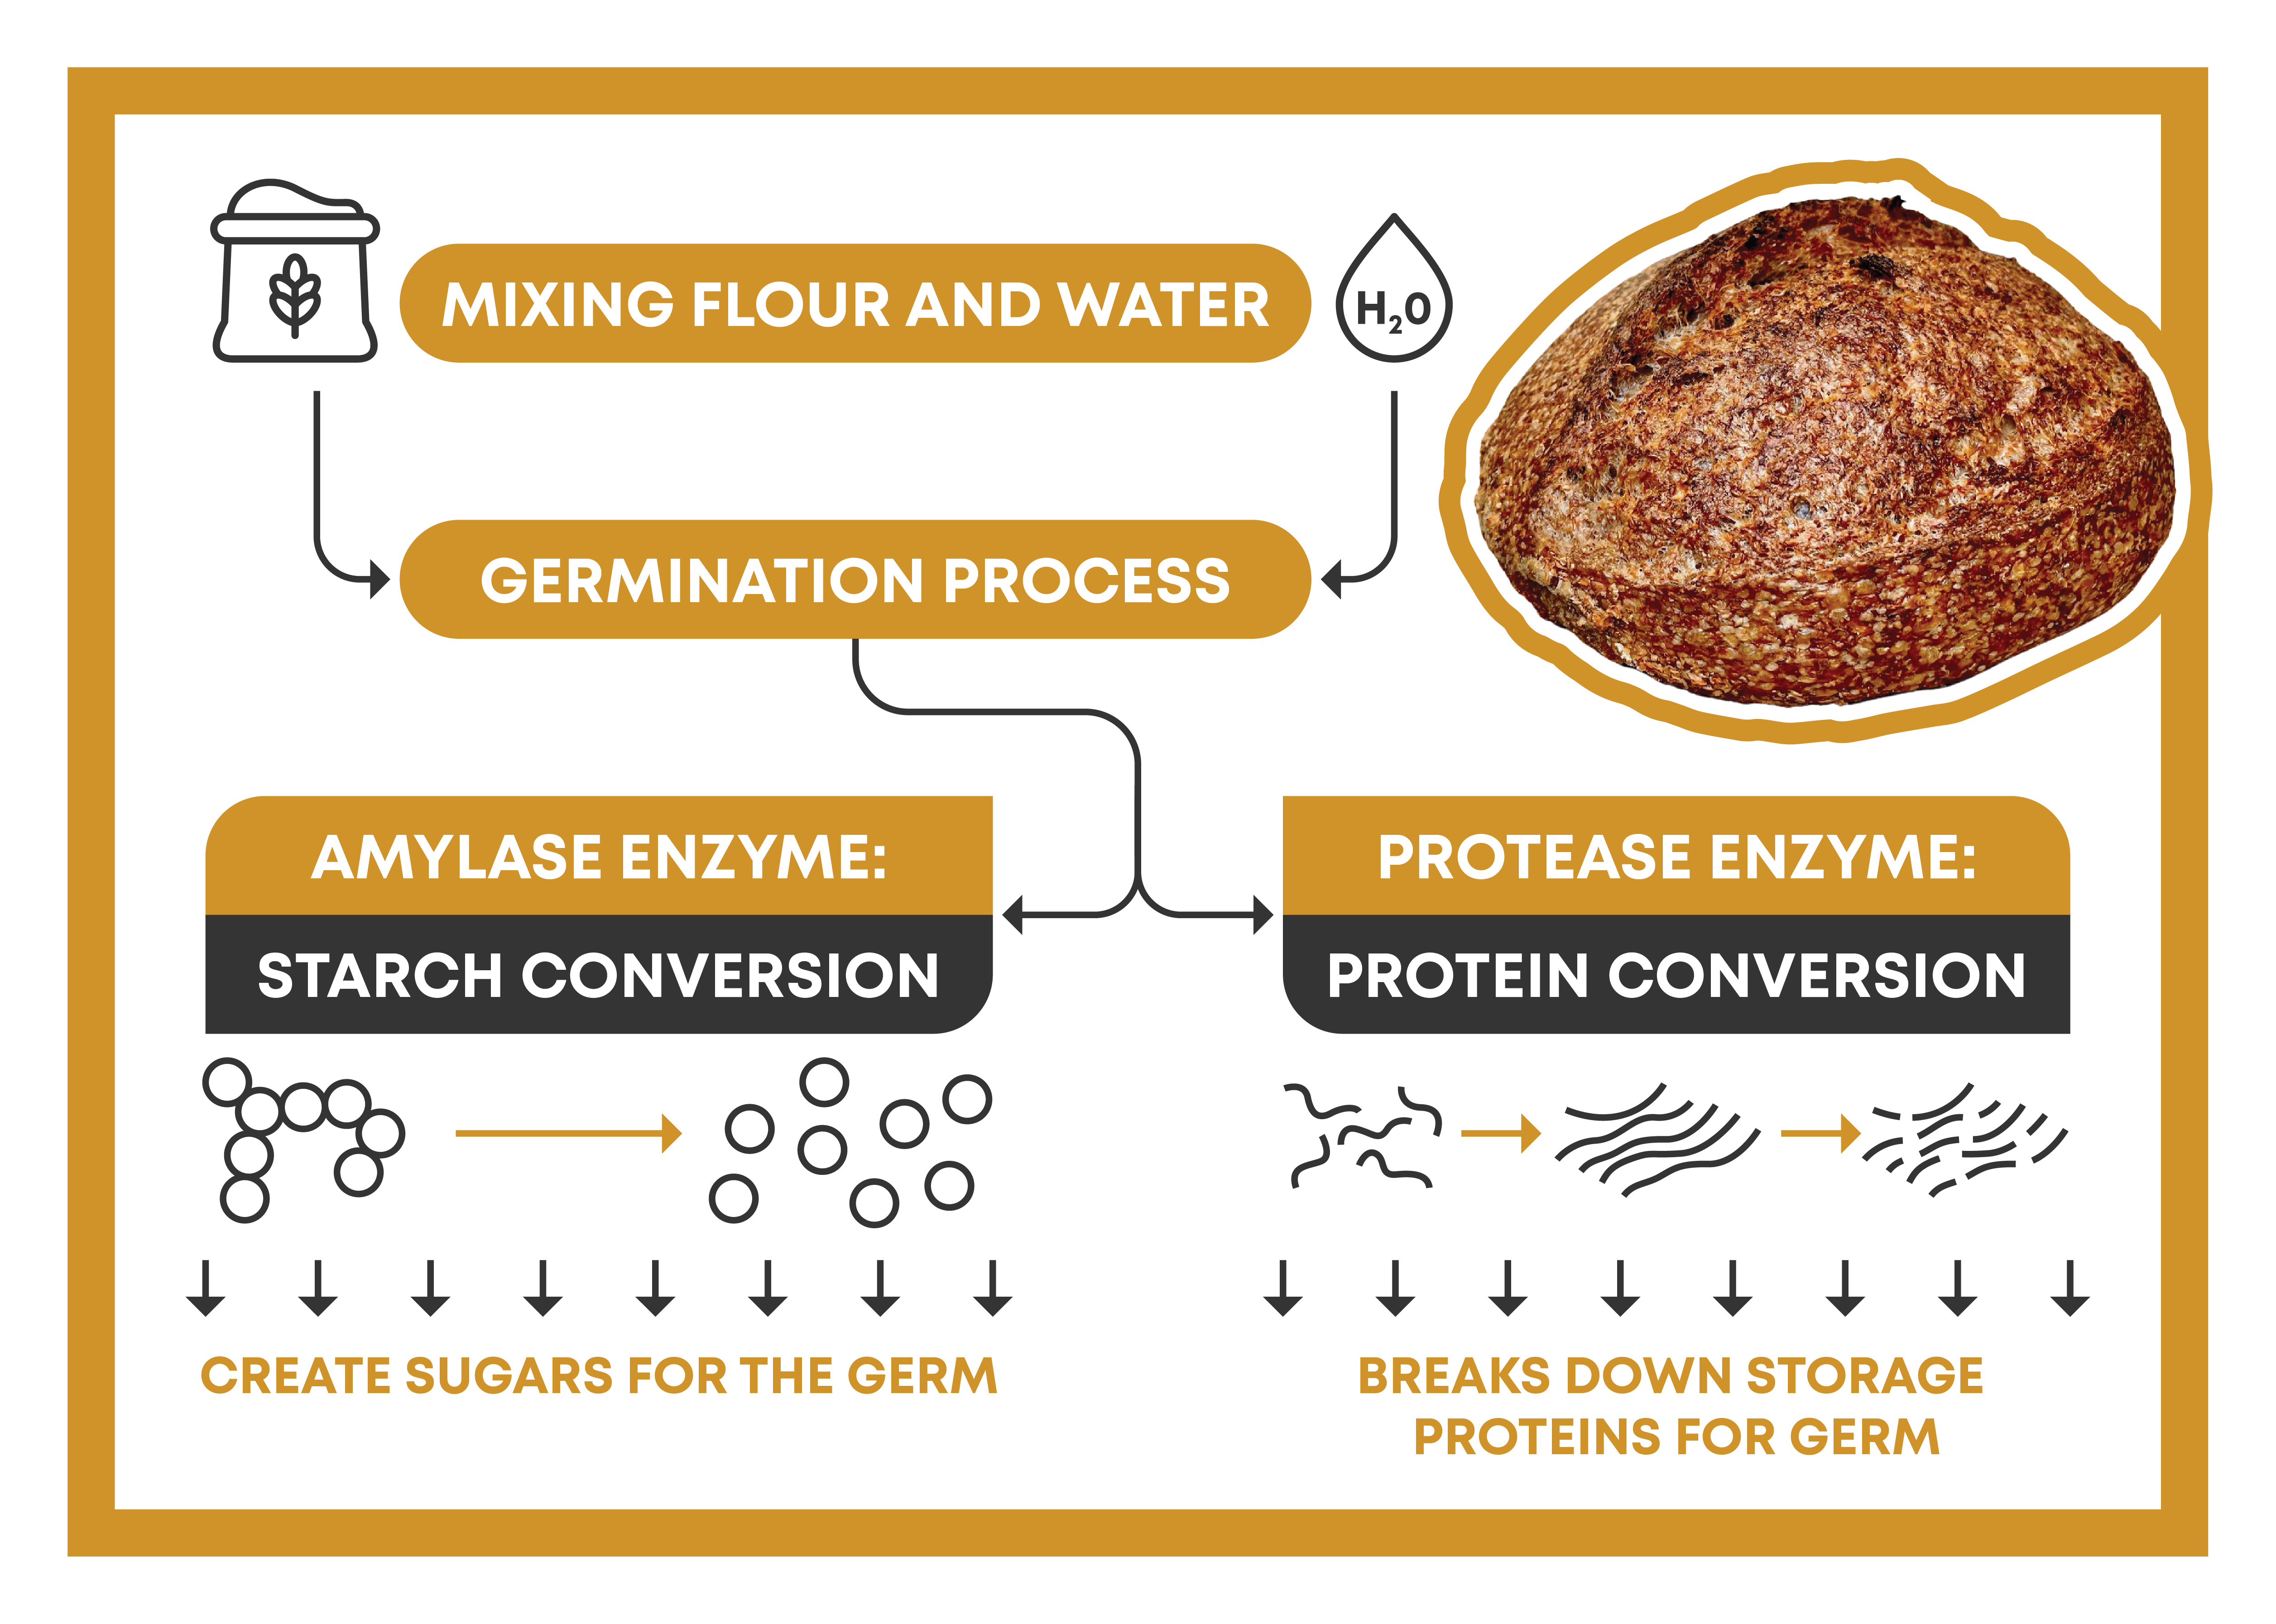
\includegraphics[width=\textwidth]{infographic-enzymes}
  \caption{How amylases and proteases interact with flour}
  \label{infographic-enzymes}
\end{figure}

\section{Enzymatic reactions}

To understand the many enzymatic reactions that take place when flour
and water are mixed, we must first understand seeds and their role in
the lifecycle of wheat and other grains.

Seeds are the primary means by which many plants, including wheat,
reproduce. Each seed contains the embryo of another plant, and must
therefore contain all the nutrients that new plant requires to grow.

When the seed is dry, it is in hibernation mode and can sometimes be
stored for several years. The moment it comes into contact with water,
however, it begins to sprout. The seed turns into a germ, requiring the
stored nutrients to be converted into something the plant can use while
it grows. The catalyst that makes the associated reactions possible is water.

The seed typically contains the first prototypical leaves of the plant,
and can put down roots using the stored nutrients inside. Once those leaves
break through the soil and come into contact with the sunlight above, they
begin to photosynthesize. This process is the plant's engine, and with the
energy photosynthesis produces, the plant can continue to grow more roots,
enabling it to access additional nutrients from the soil. These additional
nutrients allow the plant to grow more leaves, increasing its photosynthetic
activity so that it can thrive in its new environment.

Of course, a ground flour can no longer sprout. But the enzymes that
trigger this process are still present. That's why it's important not to
mill grains at too high a temperature, as doing so could damage some of
these enzymes.

Normally, the grain seed shields the germ against pathogens. However, as the
grain is ground into flour, the contents of the seed are exposed. This is ideal
for our sourdough microorganisms.

% I removed the line referencing yeast as a saprotrophic fungus since you
% cover this later on in the chapter and removing that helps the text to
% flow more smoothly.
Neither the yeast nor the bacteria can prepare their own food. However, as
the enzymes are activated, the food they need becomes available, allowing them
to feed and multiply.

The two main enzymes involved in this process are \textbf{amylase} and
\textbf{protease}. For reasons that will soon be clear, they are of the utmost
importance to the home baker, and their role in the making of sourdough is a
key puzzle piece to making better-tasting bread.

\subsection{Amylase}

Sometimes, when you chew on a potato or a piece of bread for a long period
of time, you'll perceive a sweet flavor on your tongue. That's because your
salivary glands produce amylase. Amylase breaks down complex starch molecules
into easily-digestible sugars. The germ needs this to produce more plant
matter, and your body needs this to kick-start the digestive process. Normally,
the microorganisms on the surface of the grain can't consume the freed maltose
molecules, which remain hidden inside the germ. But as we grind the flour, a
feeding frenzy takes place. Generally, the warmer the temperature, the faster
this reaction occurs. That's why a long fermentation is key to making great
bread. It takes time for the amylase to break down most of the starch into
simple sugars, which are not only consumed by the yeast but are also essential
to the \textit{Maillard reaction}, responsible for enhanced browning during the
baking process.

If you're a hobby brewer, you'll know that it's important to keep your beer at
certain temperatures to allow the different amylases to convert the contained
starches into sugar \cite{beer+amylase}. This process is so important that
there's a frequently used test to determine whether or not all the starches
have been converted.

This test, called the Iodine Starch Test, involves mixing iodine into a sample
of your brew and checking the color. If it's blue or black, you know you still
have unconverted starches. I wonder if such a test would also work for bread
dough?

Industrial bakers that add especially active yeast to produce bread in a short
period of time face a similar issue. Their approach is to add malted flour to
the dough. The malted flour contains many enzymes, and thus speeds up the
fermentation process. The next time you're at the supermarket, check the
packaging of the bread you buy. If you find {\it malt} in the list of
ingredients, chances are this strategy was used.

Note that there are actually two categories of malt. One is {\it enzymatically
active malt}, which has not been heated to above 70°C, where the amylases begin
to degrade. The other is {\it inactive malt}, which has been heated to higher
temperatures and thus has no impact on your flour.

\subsection{Protease}

Just as amylase breaks starches down into simple sugars, protease breaks
complex proteins down into simpler proteins and amino acids. Because wheat
contains gluten, a protein that's essential to the structure of bread,
protease necessarily plays a crucial role in the baking of sourdough.

Since the grain seeds require smaller amino acids to build roots and other
plant materials, the gluten in those seeds will begin to break down the moment
they sprout, and since adding water to flour activates those same enzymes,
the same process occurs in bread dough.

If you've ever tried to make a wheat-based dough and kept it at room
temperature for several days, you'll have discovered for yourself that the
gluten network breaks down so that the dough can no longer hold together. Once
this happens, the dough easily tears, holds no structure, and is no
longer suitable for baking bread.

This happened to me once when I tried to make sourdough directly from a dried
starter. At three to four days, the fermentation speed was so slow that the
gluten network broke down. The root cause for this issue was protease.

By adding water to your dough, you activate the protease, and this gets to work
in readying amino acids for the germ.

Here's another interesting experiment you can try to better visualize the
importance of protease: Make a fast-proofing dough using a large quantity
of active dry yeast. In one to two hours, your dough should have leavened and
increased in size. Bake it, then examine the crumb structure. You should see
that it's quite dense and nowhere near as fluffy as it could have been. That's
because the protease enzyme wasn't given enough time to do its job.

At the start, while kneading, a dough becomes elastic and holds together very
well. As that dough ferments, however, it becomes more loose and extensible
\cite{protease+enzyme+bread}. This is because some of the gluten bonds have
been broken down naturally by the protease through a process known as
\textit{proteolysis}. This is what makes it easier for the yeast to inflate the
dough, and it's why a long fermentation process is critical when you want to
achieve a fluffy, open crumb with your sourdough bread.

Aside from using great ingredients, the slow fermentation process is one of the
main reasons Neapolitan pizza tastes so great; because the protease creates an
extensible, easy-to-inflate dough, a soft and airy edge is achieved.

Because the fermentation process typically takes longer than eight hours, a
flour with a higher gluten content should be used. This gives the dough more
time to be broken down by the protease without negatively affecting its
elasticity. If you were to use a weaker flour, you might end up with a dough
that's broken down so much that it tears during stretching, making it
impossible to shape into a pizza pie.

Traditionally, pizza has been made with sourdough, but in modern times, it is
made with active dry yeast, as the dough stays good for a longer period of time
and is much easier to handle on a commercial scale. If you were to use
sourdough, you might have a window of thirty to ninety minutes before the dough
starts to deteriorate, both because of the protease acting for a longer period
of time and the byproducts of bacteria which we'll discuss in more detail later
in this chapter.

\subsection{Improving enzymatic activity}

As explained previously, malt is a common trick used to speed up enzymatic
activity. Personally, however, I prefer to avoid malt and instead use a
trick I learned while making whole-wheat breads.

When I first started making whole-wheat bread, I could never achieve the
crust, crumb, or texture I desired no matter what I tried. Instead, my dough
tended to overferment rather quickly. When using a white flour with a similar
gluten content, however, my bread always turned out great.

At the time, I utilized an extended autolyse, which is just a fancy word for
mixing flour and water in advance and then letting the mixture sit. Most
recipes call for it as the process gives the dough an enzymatic head start, and
in general it's a great idea. However, as an equally effective alternative,
you could simply reduce the amount of leavening agent used (in the case of
sourdough, this would be your starter). This would allow the same biochemical
reactions to occur at roughly the same rate without requiring you to mix your
dough several times. My whole wheat game improved dramatically after I stopped
autolysing my doughs.

Now that I've had time to think about it, the result I observed makes sense.
In nature, the outer parts of the seed come into contact with water first, and
only after penetrating this barrier would the water slowly find its way to the
center of the grain. The seed needs to sprout first to outcompete other nearby
seeds, requiring water to enter quickly, yet the seed must also protect itself
from other animals and potentially hazardous bacteria and fungi. A way for both
goals to be accomplished would be for most of the enzymes to exist in the outer
parts of the hull. As a result, they are activated first (source needed).
Therefore, by just adding a little bit of whole flour to your dough, you should
be able to significantly improve the enzymatic activity of your dough. That's
why, for plain white flour doughs, I usually add 10\textendash20\% whole-wheat
flour.

\begin{figure}
  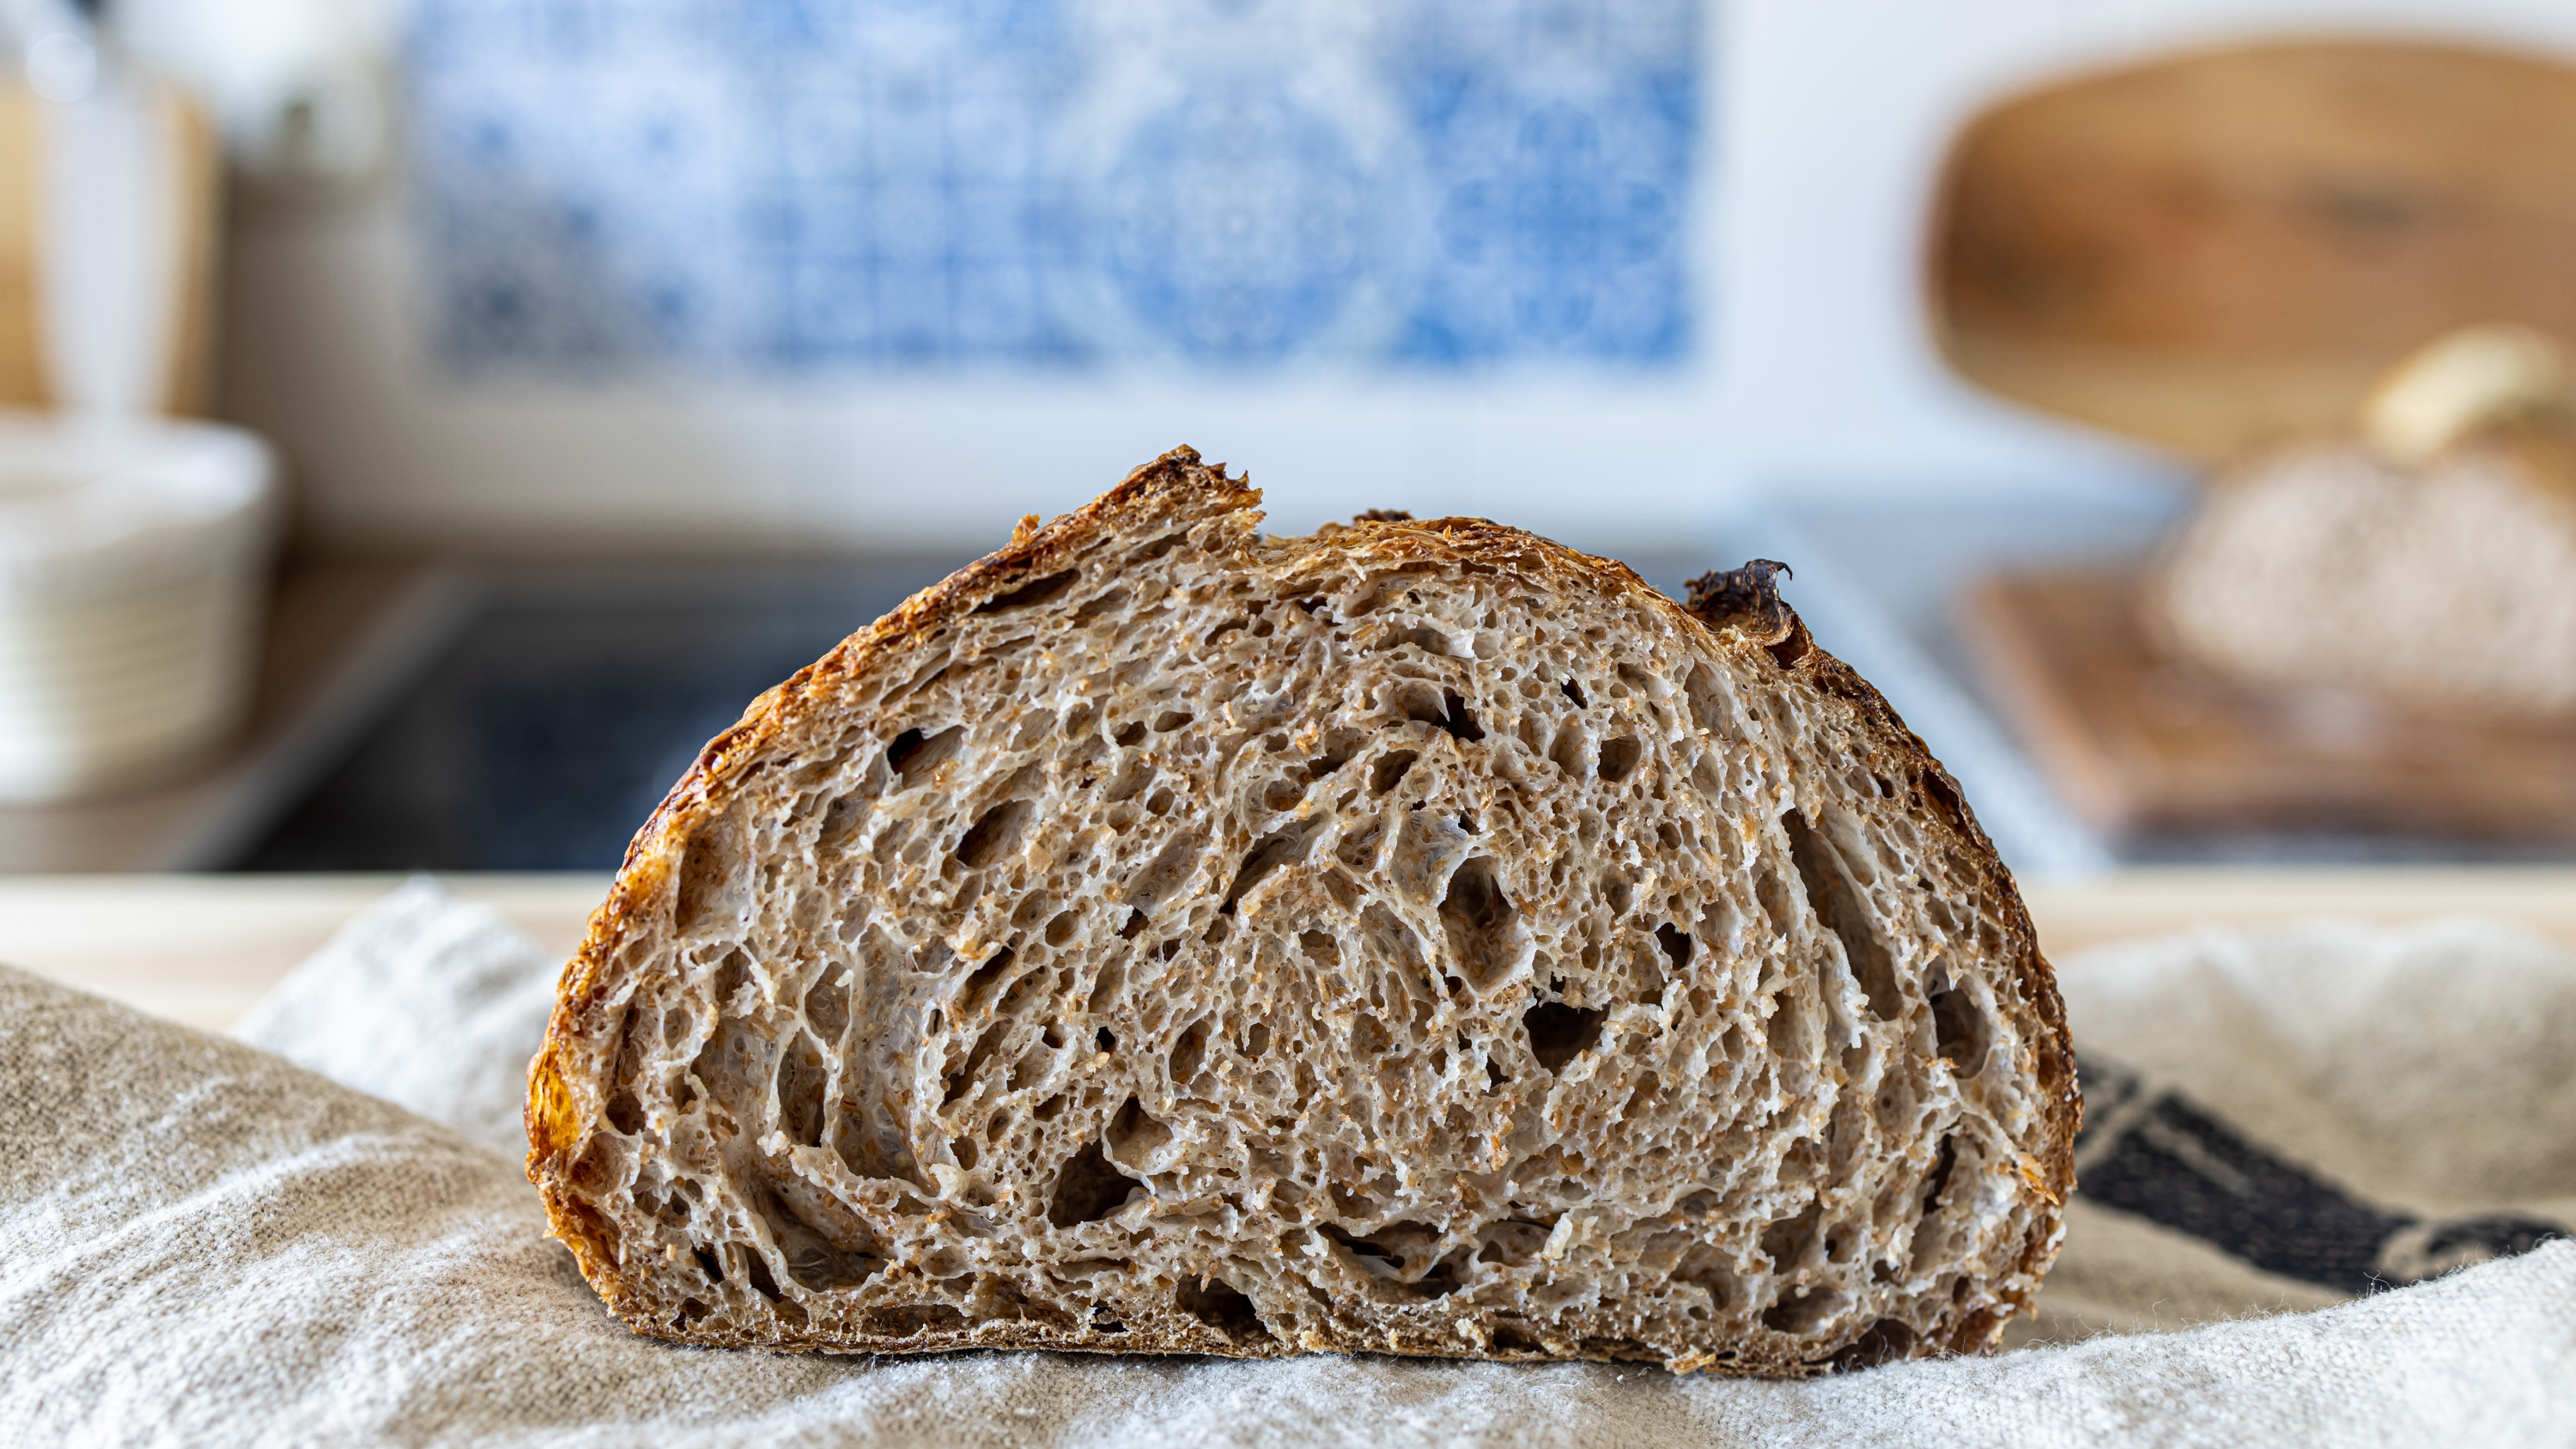
\includegraphics[width=\textwidth]{whole-wheat-crumb}
  \caption{A whole-wheat sourdough bread}
  \label{whole-wheat-crumb}
\end{figure}


By understanding the two key enzymes \textit{amylase} and \textit{protease}, you
will be better equipped to make bread to your liking. Do you prefer a softer
or stiffer crumb? Do you desire a lighter or darker crust? Do you wish to reduce
the amount of gluten in your final bread? These are all factors that you can
tweak just by adjusting the speed of your dough's fermentation.

\section{Yeast}

% Yeast is both the singular and plural form of the word unless you're
% specifically referencing a plural number of varieties or types, in which case
% "yeasts" would be correct.
Yeast are single celled microorganisms that belong to the fungi kingdom, and
spores that are hundreds of millions of years old have been identified by
scientists. There are a wide variety of species: So far, about 1,500 have been
identified. Unlike other members of the fungi kingdom such as mold, yeast do
not create a mycelium network \cite{molecular+mechanisms+yeast}.

\begin{figure}[!htb]
  \centering
  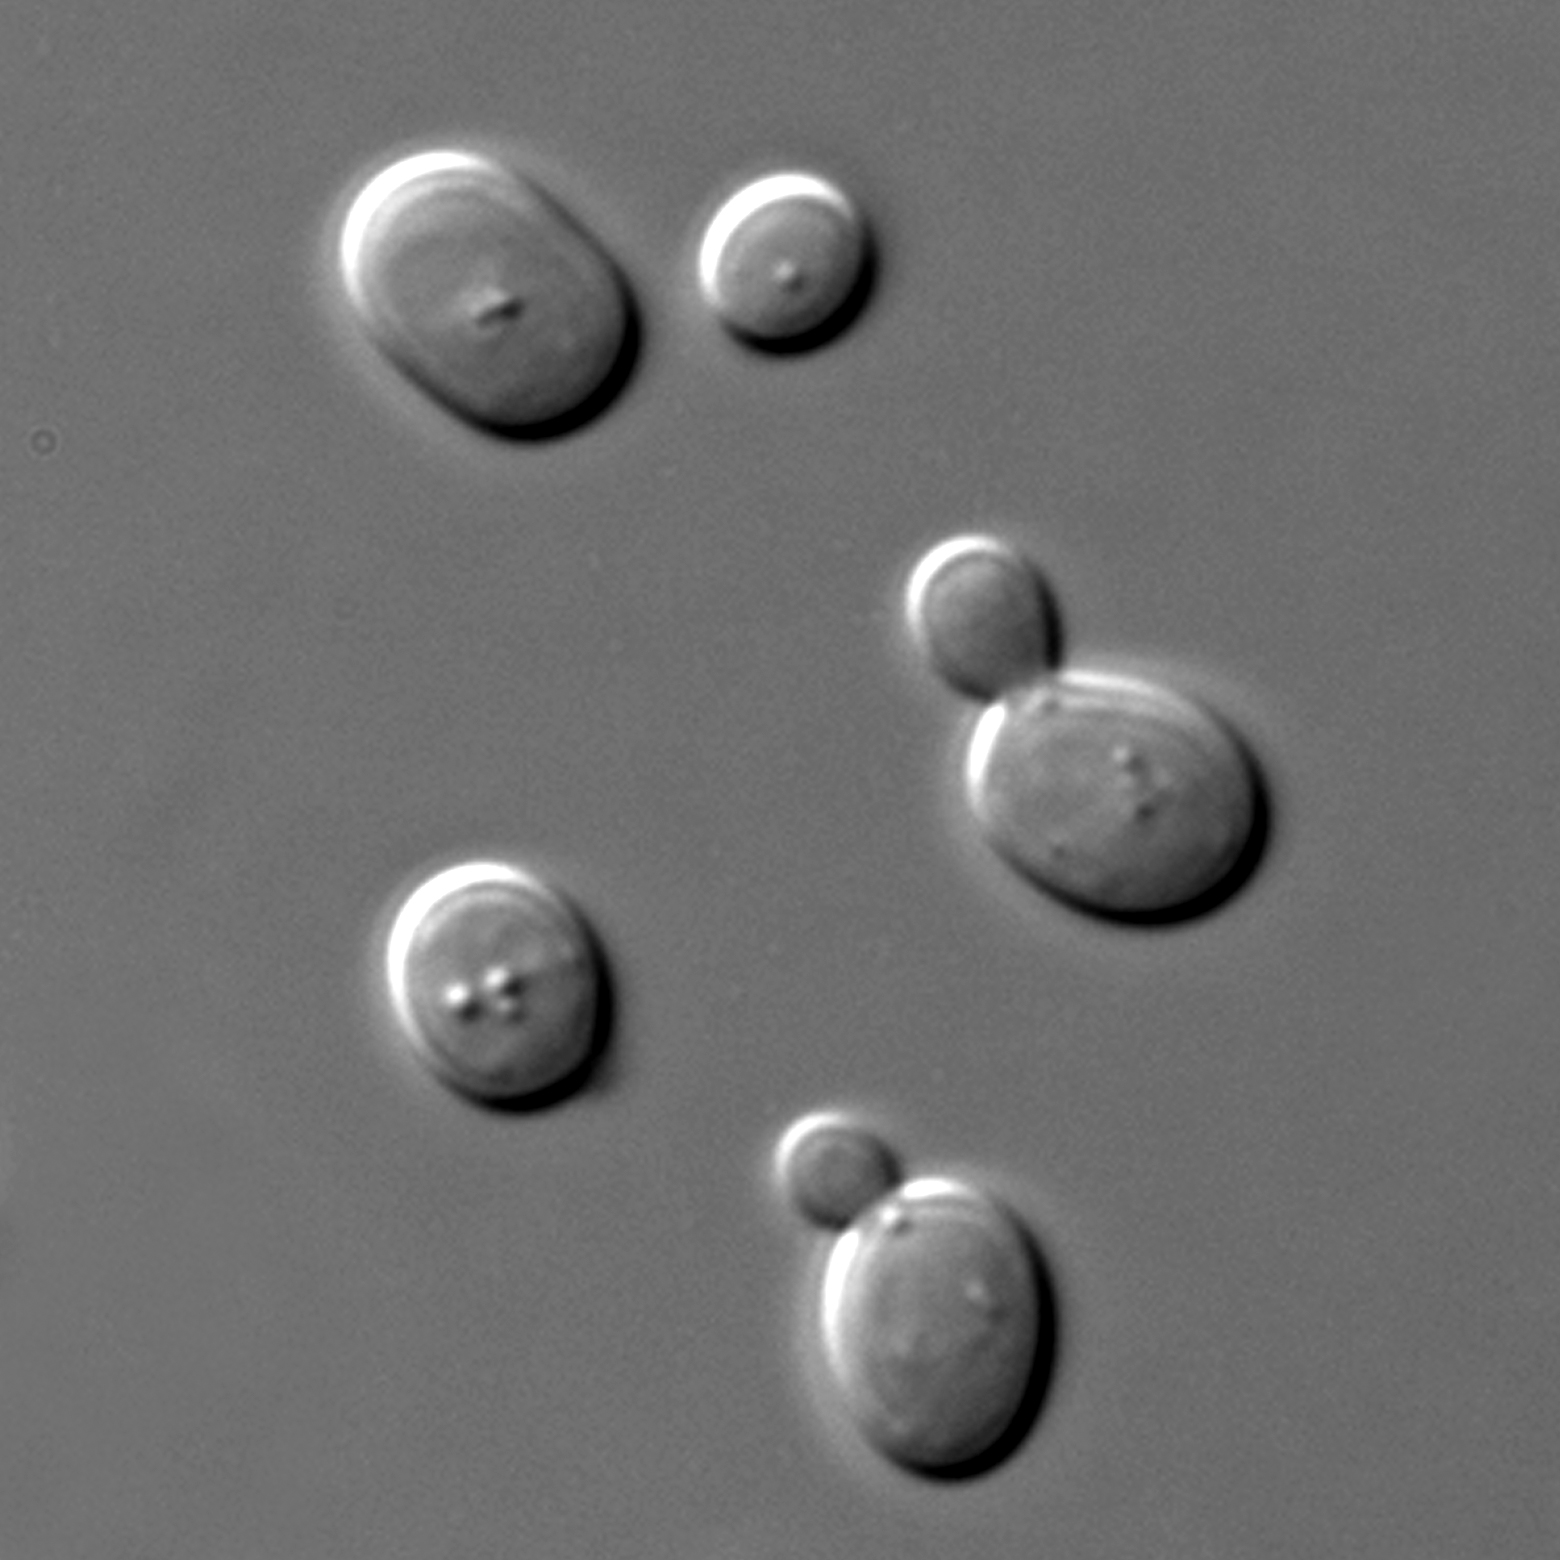
\includegraphics[width=1.0\textwidth]{saccharomyces-cerevisiae-microscope}
  \caption{Saccharomyces cerevisiae: Brewer's yeast under the microscope}
  \label{saccharomyces-cerevisiae-microscope}
\end{figure}

Yeast are saprotrophic fungi. This means that they do not produce their own
food, but instead rely on external sources that they can decompose and break
down into compounds that are more easily metabolized.

Yeast breaks down carbohydrates into carbon dioxide and alcohol in what we now
refer to as the fermentation process. This process has been known for thousands
of years and has been used since ancient times for the making of bread as well
as alcoholic beverages.

Yeast can grow and multiply under both aerobic and anaerobic conditions. When oxygen
is present the yeast almost completely produces
carbon dioxide and water. When no oxygen is present
the yeast starts switches its metabolism. The
yeast starts to produce alcoholic compounds \cite{effects+oxygen+yeast+growth}.
The temperatures at which the yeast grows vary. Some
yeasts such as {\it Leucosporidium frigidum} grows
best at temperatures between -2°C up to 20°C. Other
yeast grows better at higher temperatures. The warmer
it is the faster the yeast's metabolism works. The yeast
that you cultivate in your sourdough starter works best
at the temperatures where the grain was grown and at
the point when it was harvested. So if you are from a 
cooler place and cultivate a sourdough starter from
a nordic rye variety, then chances are your yeast
prefers this colder environment. As an example
beer makers discovered that a beneficial yeast lives
in the cold caves around the city of Pilsen, Czech Republic.
This yeast has produced excellent tasting beers at
lower temperatures. Varieties of these strains
are now used to make popular lager beers.

Yeasts in general are very common in the environment.
They can be found on cereal grains, fruits, other plants
in the soil and also in your gut. Very little is known
about the ecology of why yeasts we use for baking
are cultivating the leaves of the plants. The plants
are protected via the cell walls and hardly any
fungi and other bacteria can penetrate. Some fungi and
bacteria are producing enzymes that are able
to break down the cell walls and infect the plant.
There are fungi and bacteria that live within the plant
without causing any distress. These are known as {\it endophytes}.
They are not damaging the plant per se. In fact they are
living in a symbiotic relationship with the host. They
help the plant to protect itself from additional pathogens
that might enter through the leaves of the plant. They
help with water stress, heat stress and nutrient availability. 
In exchange for the service they receive carbon for energy
from the plant host. They are not always strictly mutualistic though.
Sometimes under stress conditions they can become pathogens
on their own \cite{endophytes+in+plants} and decay begin
decaying the plant.

The yeasts we use for baking are
living as as epiphytes on the plant. Compared to
the previously mentioned endophytes they are not
breaching the walls of the cells. Most of them
receive nutrients from rain water, the air or other animals.
These sources also include honeydew produced
by aphids. Pollen that lands on the leaf's surface
is an additional source of food. Interestingly
though when you remove that external food source,
you still find a large variety of epiphytic fungi
and bacteria on the plant's surface. The food
for them is coming directly from the plant it seems.
Some research has shown that the plants are
on purpose releasing some compounds such as sugars,
organic acids, amino acids, some methanol and various
salts via the surface. These nutrients would
then attract the epiphytes to live on the surface.
The plants benefit from enhanced protection against
mold and other pathogens. It is in the best interest
of the epiphytes to keep the plants alive
as long as possible \cite{leaf+surface+sugars+epiphytes}.
More and more research is conducted on using yeasts
as a biocontrol agents to protect plants. These bio-agents
would be food-safe as yeasts are generally considered save.
The yeasts would start to grow on the leaves on the plant
and essentially shield the plants from other molds. This
could be a game changer for wineyeards suffering from mildew.
This could also be helpful to shield the plant against the
psychoactive ergot fungus. The ergot fungus likes to grow
in more humid colder environments and poses a huge
problem to rye farmers. The fungus parasites the plant
and infects it. Consumption of ergot is not recommended
as it is highly toxic to the liver. That's why lawmakers
have recently reduced the amount of allowed ergot contamination
in rye flour. Another interesting experiment from Italian scientists
visualized how important yeasts could be when protecting
plants. They added tiny incisions into some of the grapes.
They would then infect some of the damaged surfaces with
mold. The other wounds they infected with some of the 150
different wild yeast strains isolated from the leaves plus
the mold. When mixing the mold with the yeast the grape
sustained no significant damage \cite{yeasts+biocontrol+agent}.
In another experiment however scientists have shown
how the brewer's yeast became an aggressive pathogen to wine plants.
Initially the yeast lived in symbiosis with the plant. After the grapevine
sustained damages the yeast became opportunistic and started to
attack the plant event producing hyphae to deeply
penetrate the plants tissue.

\section{Bacteria}

\chapter{Making a sourdough starter}
\chapter{Making a sourdough starter}%
\label{chapter:sourdough-starter}
\begin{quoting}

\begin{figure}[!htb]
  \centering
  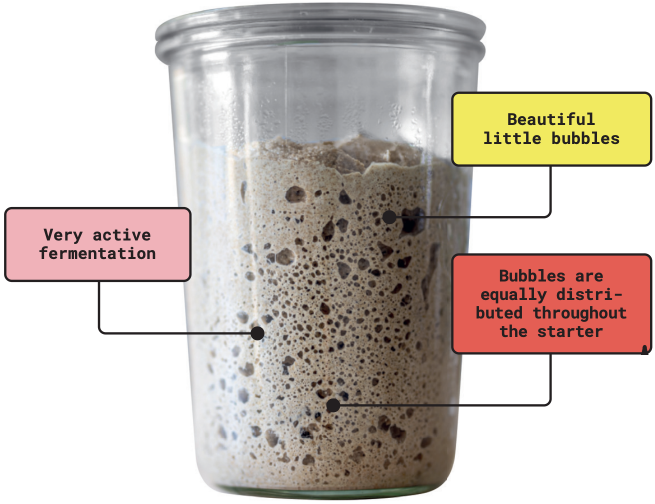
\includegraphics[width=\textwidth]{sourdough-starter-activity-indicators}
  \caption[Very active sourdough]{A very active sourdough starter shown by the
      bubbles in the dough.}%
  \label{fig:sourdough-starter}
\end{figure}

In this chapter you will learn how to make your
own sourdough starter, but before doing so you will
quickly learn about baker's math. Don't worry,
it's a very simple way how to write a recipe which
is cleaner and more scalable. Once you get the hang
of it you will want to write every recipe this way.
You will learn to understand the signs indicating
your starter's readiness, as well as
how to prepare your starter for long-term storage.
\end{quoting}

\iffalse

\section{Baker's math}%
\label{section:bakers-math}

In a large bakery, a determining factor is how
much flour you have at hand. Based on the amount
of flour you have, you can calculate how many
loaves or buns you can make. To make it easy
for bakers, the quantity of each ingredient
is calculated as a percentage based on how much flour you have.
Let me demonstrate this with a small example from
a pizzeria. In the morning you check and you realize you
have around \qty{1}{\kg} of flour.
Your default recipe calls for around \qty{600}{\gram} of water.
That would be a typical pizza dough, not too dry but
also not too wet. Then you would be using around \qty{20}{\gram}
of salt and around \qty{100}{\gram} of sourdough starter\footnote{This is my go to
pizza dough recipe. In Napoli modern pizzerias would use fresh or dry yeast.
However traditionally pizza has always been made with sourdough.}.
The next day you suddenly have \qty{1.4}{\kg} of flour
at hand and thus can make more pizza dough. What do you do?
Do you multiply all the ingredients by \num{1.4}? Yes you could,
but there is an easier way. This is where baker's math
comes in handy. Let's look at the default recipe with baker's
math and then adjust it for the \qty{1.4}{\kg} flour quantity.

\begin{table}[!htb]
\centering
  \begin{tabular}{@{}r@{g }lrr@{ = }r@{}}
\toprule
\multicolumn{2}{c}{\thead{Ingredient}}& \thead{Percentage} & \multicolumn{2}{c}{\thead{Calculation}} \\ \midrule
1000& flour             &100\%        & 1000g of 1000g & 100\% \\ 
 600& water             & 60\%        & 600g of 1000g  &  60\% \\ 
 100& sourdough starter & 10\%        & 100g of 1000g  &  10\% \\ 
  20& salt              &  2\%         & 20g of 1000g  &   2\% \\ \bottomrule
\end{tabular}

  \caption[Baker's math example]{An example table demonstrating how to
      properly calculate using baker's math}
\end{table}

Note how each of the ingredients is calculated as a percentage
based on the flour. The \qty{100}{\percent} is the baseline and represents the absolute
amount of flour that you have at hand. In this case that's
\qty{1000}{\gram}~(\qty{1}{\kg}).

Now let's go back to our example and adjust the flour, as we have
more flour available the next day. As mentioned the next day
we have \qty{1.4}{\kg} at hand (\qty{1400}{\gram}).

\begin{table}[!htb]
    \centering
        \begin{tabular}{@{}lrr@{ = }l@{}}
\toprule
\thead{Ingredient} & \thead{Baker's math} & \multicolumn{2}{c}{\thead{Calculated value}} \\ \midrule
Flour               & 100\%   & $1400 \times 1$ & 1400g         \\ \midrule
Water               & 60\%    & $1400 \times 0.6$ & 840g        \\ \midrule
Sourdough starter   & 10\%    & $1400 \times 0.1$ & 140g        \\ \midrule
Salt                & 2\%     & $1400 \times 0.02$ & 28g        \\ \bottomrule
\end{tabular}

        \caption[Another baker's math example]{An example recipe that uses
            \qty{1400}{\gram} as its baseline and is then calculated using
            baker's math.}
\end{table}

For each ingredient we calculate the percentage
based on the flour available (\qty{1400}{\gram}). So for the water
we calculate \qty{60}{\percent} based on \num{1400}. Open up your
calculator and type in \numproduct{1400 x 0.6} and you have
the exact value in grams that you should be using.
For the second day, that is \qty{840}{\gram}. Proceed to do the same
thing for all the other ingredients and you will know
your recipe.

Let's say you would want to use \qty{50}{\kg} of flour
the next day. What would you do? You would simply proceed
to calculate the percentages one more time. I~like this
way of writing recipes a lot. Imagine you wanted to make
some pasta. You would like to know how much sauce you should
be making. Now rather than making a recipe just for you, a
hungry family arrives. You are tasked with making pasta
for \num{20} people. How would you calculate the amount of sauce
you need? You go to the internet and check a recipe and then
are completely lost when trying to scale it up.
\fi

\section{The process of making a starter}

Making a sourdough starter is very easy, all you need
is a little bit of patience. It is in fact so easy that it can be summarized
in a simple flowchart~\ref{fig:sourdough-starter-process}.

\begin{flowchart}[!htb]
\centering
  \begin{tikzpicture}[node distance = 3.5cm, auto]
  \node [start] (init) {Mix \qty{50}{\gram} flour + \qty{50}{\gram} water, stir};
  \node [block, right of=init] (wait2) {Wait\\ \qty{24}{\hour}};
  \path [line] (init) -- (wait2);
  \node [block, below of=wait2, node distance=3.5cm] (feed) {\qty{10}{\gram} of previous day + \qty{50}{\gram} water + \qty{50}{\gram} flour, stir};
  \path [line] (wait2) -- (feed);
  \node [block, below of=feed] (discard) {Discard the rest};
  \path [line] (feed) -- (discard);
  \node [decision, right of=feed, node distance=3.5cm] (decide) {Is good?};
  \node [decision, above of=decide, node distance=3.5cm] (timeout) {Less than 10 feeds?};
  \node [fail, right of=timeout, node distance=3.5cm] (discard2) {Batch failed};
  \path [line] (timeout) -- node{no} (discard2);
  \path [line] (timeout) -- node{yes} (wait2);
  \path [line] (feed) -- (decide);
  \node [success, right of=decide, node distance=3.5cm] (use) {Ready to use};
  \path [line] (decide) -- node{no} (timeout);
  \path [line] (wait2) -- (feed);
  \path [line] (decide) -- node{yes} (use);

  \node [start, below of=discard, left of=discard] (start_n) { Start with Initial Mixture };
  \node [block, right of=start_n, node distance = 3.2cm] (wait_n) { Wait\\ \qty{24}{\hour} };
  \node [decision, right of=wait_n, node distance = 3.2cm] (readycheck_n) { Ready? };
  \node [block, below of=wait_n, node distance = 3cm] (feed_n) { Feed the Mixture };
  \node [decision, right of=feed_n, node distance = 3.2cm] (limitcheck_n) { Failed? };
  \node [fail, right of=limitcheck_n, node distance = 3.2cm] (abort_n) { Discard All, Start Over };
  \node [success, right of=readycheck_n, node distance = 3.2cm] (final_n) { Done };

  \draw [line] (start_n) -- (wait_n);
  \draw [line] (wait_n) -- (readycheck_n);
  \draw [line] (feed_n) -- (wait_n);
  \draw [line] (readycheck_n) -- node { No } (limitcheck_n);
  \draw [line] (limitcheck_n) -- node (feedok_n) { No } (feed_n) ;
  \draw [line] (limitcheck_n) -- node { Yes } (abort_n);
  \draw [line] (readycheck_n) -- node { Yes } (final_n);

  \node [below of=feedok_n, node distance=2cm, align=left] (details2) [shape=rectangle,draw,fill=white!90!black]{
    \fontsize{7}{9}\selectfont For the \emph{Initial Mixture}, mix \qty{50}{\gram} flour/\qty{50}{\gram} water.\\
    \fontsize{7}{9}\selectfont The Mixture is \emph{Ready} when it has
    \emph{grown}, has \emph{bubbles}, and \emph{smells}
    vinegary/yoghurty. \\

    \fontsize{7}{9}\selectfont The Mixture has \emph{Failed} when you
    have fed it too many (eg 10) times without success.\\

    \fontsize{7}{9}\selectfont To \emph{Feed the Mixture}, discard all but \qty{10}{\gram}, mix in \qty{50}{\gram} flour and \qty{50}{\gram} water.
  };
\end{tikzpicture}

  \caption[The full sourdough starter process]{The process of making a sourdough
      starter from scratch.}%
  \label{fig:sourdough-starter-process}
\end{flowchart}

The flour you should
use to bootstrap your starter is ideally a whole flour.
You could use whole-wheat, whole-rye, whole-spelt or
any other flour you have. In fact gluten free flours such
as rice or corn would also work. Don't worry, you can always
change the flour later. Use whatever whole flour you
already have at hand.

Your flour is contaminated with millions of microbes. As explained
before in the chapter about wild yeast and bacteria, these
microbes live on the surface of the plant. That's why
a whole flour works better because you have more natural
contamination from the microbes you are trying to cultivate
in your starter. More of them live on the hull compared to the
endophytes living in the grain.

Start by measuring approximately \qty{50}{\gram} of both flour and
water. The measurements don't have to be exact; you can use
less or more, or just eyeball the proportions. These
values are just shown as a reference.

Don't use chlorinated water when setting up your starter.
Ideally, you should use bottled water. In certain regions
like Germany, tap water is perfectly fine. Chlorine is added
to water as a disinfectant to kill microorganisms, you will
not be able to grow a starter with chlorinated water.

In this process, the hydration of your starter is \qty{100}{\percent}.
This means you're using equal amount of flour and
water. Stir everything together so that all the flour is
properly hydrated. This step activates the microbial spores
in your mixture, drawing them out of hibernation and
reviving them.
Finally, cover your mixture but make sure the covering is
not airtight. You still want some gas exchange to be possible.
I~like to use a glass and place another
inverted one on top.

Now an epic battle begins. In one study~\cite{yeasts+biocontrol+agent}
scientists have identified more than \num{150}~different yeast species living
on a single leaf of a plant.
All of the different yeasts and bacteria are trying to get
the upper hand in this battle. Other pathogens such as mold
are also being activated as we added water. Only the strongest
most adaptable microorganisms will survive.

\begin{figure}[!htb]
  \includegraphics[width=\textwidth]{sourdough-starter-microbial-war}
  \caption[Microbial warfare during sourdough early days]{A simple
      visualization of the microbial warfare that happens during the making of
      a sourdough starter. The wild spores on the plant and flour become
      activated the moment flour and water is mixed.  Only the most adapted
      flour-fermenting microbes will survive. Because of unwanted microbial
      fermentation it is advised to discard the feeding-leftovers of the first
      days. The surviving yeast and bacteria continuously try to outcompete
      each other for resources. New microbes have a hard time entering the
      starter and are eliminated.}%
  \label{fig:sourdough-starter-microbial-war}
\end{figure}

By adding water to the
flour the starches start to degrade. The seedling tries to
sprout but it no longer can. Essential for this process is the
amylase enzyme. The compact starch is broken down to more
digestible sugars to fuel plant growth. Glucose is what the
plant needs in order to grow. The microorganisms that survive
this frenzy are adapted to consuming glucose. 

Luckily for us
bakers, the yeast and bacteria know very well how to metabolize
glucose. This is what they have been fed in the wild by the plants.
By forming patches on the leaf and protecting the plant from
pathogens they received glucose in return for their services.
Each of the microbes tries to defeat the other by consuming the
food fastest, producing agents to inhibit food uptake by others or by producing
bactericides and/or fungicides. This early stage of the starter
is very interesting as more research could possibly reveal
new fungicides or antibiotics. 

Depending on where your flour
is from, the starting microbes of your starter might be different
than the ones from another starter. Some people have also reported
how the microbes from your hand or air can influence your starter's
microorganisms. This makes sense to a certain extent. Your
hand's microbes might be good at fermenting your sweat, but
probably not so good at metabolizing glucose. The contamination
of your hands or air might play a minor role in the initial epic
battle. But only the fittest microbes fitting the sourdough's
niche are going to survive. 

This means the microorganisms knowing
how to convert maltose or glucose will have the upper hand. Or the
microbes fermenting the waste of the other microbes. Ethanol created
by the yeast is metabolized by the bacteria in your sourdough. That's
why a sourdough has no alcohol. I~can confirm the role of aerial
contamination to a certain extent, when setting up a new sourdough
starter the whole process is quite quick for me. After a few
days my new starter seems to be quite alive already. This might
be due to previous contamination of flour fermenting microbes in
my kitchen.

Wait for around 24~hours and observe what happens to your starter.
You might see some early signs of fermentation already. Use your nose
to smell the dough. Look for bubbles in the dough. Your dough
might already have increased in size a little bit. Whatever
you see and notice is a sign of the first battle.

Some microbes
have already been outperformed. Others have won the first battle.
After around 24~hours most of the starch has been broken down
and your microbes are hungry for additional sugars. With a spoon
take around \qty{10}{\gram} from the previous day's mixture and place
it in a new container. Again --- you could also simply eye ball
all the quantities. It does not matter that much. Mix the \qty{10}{\gram}
from the previous day with another \qty{50}{\gram} of flour
and \qty{50}{\gram} of water. 

Note the ratio of 1:5. I~very often use
1~part of old culture with 5~parts of flour and 5~parts of water.
This is also very often the same ratio I~use when making a dough.
A dough is nothing else than a giant sourdough starter with slightly different
properties. I'd always be using around \qtyrange{100}{200}{\gram} of starter
for around \qty{1000}{\gram} of flour (baker's math: \qtyrange{10}{20}{\percent}).

Homogenize your new mixture again with a spoon. Then cover
the mix again with a glass or a lid. If you notice the top of
your mixture dries out a lot consider using another cover. The
dried-out parts will be composted by more adapted microbes such as
mold. In many user reports, I~saw mold being able to damage
the starter when the starter itself dried out a lot. 

You will
still have some mixture left from your first day. As this contains
possibly dangerous pathogens that have been activated make sure you discard
this mixture. A rule of thumb is to begin keeping the discard,
the moment you made your first successful bread. At that point
your discard is long-fermented flour that is an excellent addon
used to make crackers, pancakes or delicious hearty sandwich
bread\ldots I~also frequently dry it and use it as a rolling agent
for pizzas that I~am making.\footnote{Discarding starter when preparing
a new batch can be frustrating. With experience, bread-making
becomes more efficient, and excess discard is rarely produced. It is
possible to prepare just the right amount of starter
needed for bread dough. In fact, a fully depleted starter can even be revived
using a small portion of bread dough. Any leftover discard, rich in spores,
can also serve as a backup to create a new sourdough starter. Simply mix the
discard with a little flour and water, and it will spring back to life. That is a
great option if the starter was accidentally depleted. A practical approach
is to store all discard in a single jar in the fridge, adding new discard on
top as needed and using it whenever required.}

You should hopefully again see some bubbles, the starter increasing
in size and/or the starter changing its smell. Some people give
up after the second or third day, because the signs might no longer
be as dominant as they were on day one. The reason for this lies in only a few
select microbes starting to take over the whole sourdough starter. The most
adaptable ones are going to win, they are very small in quantity and will
grow in population with each subsequent feeding. Even if you see no signs
of activity directly, do not worry, there is activity in
your starter at a microscopic level.

24~hours later again we will repeat the same thing again until
we see that our sourdough starter is active. More on that in the
next section of this book.

\section{Determining starter readiness}

For some people the whole process of setting up a starter takes
only 4~days. For others it can take 7~days, for some even 20~days.
This depends on several factors including how good your wild microbes
are at fermenting flour. Generally speaking, with each feeding
your starter becomes more adapted to its environment. Your
starter will become better at fermenting flour. That's why
a very old and mature starter you receive from a friend might
be stronger than your own starter initially. Over time
your sourdough starter will catch up. Similarly, modern baking
yeast has been isolated like this from century old sourdough
starters.

\begin{flowchart}[!htb]
\centering
  \documentclass[tikz]{standalone}
\usepackage{tikz}
\usepackage{siunitx}
\DeclareSIUnit\degF{\text{°}F}

\begin{document}
\begin{tikzpicture}[node distance = 3cm, auto]
  \node [block] (init) {\footnotesize Make a starter};
  \node [block, right of=init, node distance=3cm] (feed) {\footnotesize Feed your starter};
  \path [line] (init) -- (feed);
  \node [block, right of=feed, node distance=3cm] (wait_12_after_feed) {\footnotesize Wait 12 hours};
  \path [line] (feed) -- (wait_12_after_feed);
  \node [block, right of=wait_12_after_feed, node distance=3cm] (ready_question) {\footnotesize Perform readiness check};
  \path [line] (wait_12_after_feed) -- (ready_question);
  \node [block, below of=feed, node distance=3cm] (wait_12) {\footnotesize Wait 12 hours};
  \path [line] (wait_12) -- (feed);
  \node [decision, right of=ready_question, node distance=3.5cm] (is_bubbly) {\footnotesize Bubbly? Size Increase?};
  \path [line] (ready_question) -- (is_bubbly);
  \path [line] (is_bubbly) -- node{no} (wait_12);
  \node [decision, below of=is_bubbly, node distance=4.0cm] (check_smell) {\footnotesize Vinegary, or yogurt smell?};
  \path [line] (is_bubbly) -- node{yes} (check_smell);
  \node [block, below of=init, node distance=6cm] (make_dough) {\footnotesize Make your dough};
  \path [line] (check_smell) -- node{yes} (make_dough);
  \path [line] (check_smell) -- node{no} (wait_12);
\end{tikzpicture}
\end{document}

  \caption[Determining sourdough starter readiness]{A flow chart showing you how to
      determine if your sourdough starter is ready to be used. Make sure to
      wait at least \qtyrange{6}{12}{\hour} after feeding your
      starter to check its readiness. To evaluate it, look at your starter's size
      increase, airy texture and take note of its smell.
      All three factors are important to properly evaluate your starter's activity level.
      An active starter is an important foundation for a successful dough fermentation}%
  \label{fig:sourdough-starter-readiness}
\end{flowchart}

The key sign to look at is bubbles that you see in your starter
jar. This is a sign that the yeast is metabolizing your
dough and creates \ch{CO2}. The \ch{CO2} is trapped in your dough
matrix and then visualized on the edges of the container.

Also note the size increase of your dough. The amount the dough increases
in size is irrelevant. Some bakers claim it doubles, triples or quadruples.
The amount of size increase depends on your microbes, but also on
the flour that you use to make the starter. Wheat flour contains
more gluten and will thus result in a larger size increase. At
the same time the microbes are probably not more active compared
to when living in rye sourdough. You could only argue that
wheat microbes might be better at breaking down gluten compared
to rye microbes. That's one of the reasons why I~decided to change
the flour of my sourdough starter quite often. I~had hoped to create
an all-around starter that can ferment all sorts of different
flour\footnote{Whether this is working, I~can't scientifically say.
Typically the microbes that have once taken place are very strong
and won't allow other microbes to enter. My starter has initially
been made with rye flour. So chances are that the majority of
my microorganisms are from a rye source.}.

Your nose is also
a great tool to determine starter readiness. Depending on
your starter's microbiome you should notice either the smell
of lactic acid or acetic acid. Lactic acid has dairy yogurty notes.
The acetic acid has very strong pungent vinegary notes. Some
describe the smell as glue or acetone. Combining the visual clues
of size increase and pockets plus the smell is the best way
to determine starter readiness.

In rare events your flour might be treated and prevent microbe growth.
This can happen if the flour is not organic and a lot of biochemical
agents have been used by the farmer. In that case simply try again
with different flour. Ten~days is a good period of time to wait before
trying again.

Another methodology used by some bakers is the so called \emph{float test}.
The idea is to take a piece of your sourdough starter and place it
on top of some water, if the dough is full with gas it will float
on top of the water. If it's not ready, it can't float and will
sink to the bottom. This test does not work with every flour,
rye flour for instance can't retain the gas as well as wheat flour
and thus in some cases will not float. That's why I~personally
don't use this test and can't recommend it.

Once you see your starter is ready I~would recommend giving it
one last feeding and then you are ready to make your dough in the
evening or the next day. For the instructions on how to make your
first dough please refer to the next chapters (\ref{chapter:wheat-sourdough}
and~\ref{chapter:non-wheat-sourdough}) in this book.

If your first bread failed, chances are your fermentation hasn't
worked as expected. In many cases the reason is your sourdough starter. Maybe
the balance of bacteria and yeast isn't optimal yet. In that case a good
solution is to keep feeding your starter once per day. With each feeding your
starter becomes better at fermenting flour. The microbes will adapt more and
more to the environment. Please also consider reading the stiff sourdough starter
chapter in this book. The stiff sourdough starter helps to boost the
yeast part of your sourdough and balance the fermentation.

\section{Maintenance}

\begin{flowchart}[!htb]
\centering
  \documentclass[tikz]{standalone}
\usepackage{tikz}
\usepackage{siunitx}
\DeclareSIUnit\degF{\text{°}F}

\begin{document}
\begin{tikzpicture}[node distance = 3cm, auto]
  \node [block] (init) {\footnotesize Make your bread dough};
  \node [decision, below of=init, node distance=3.5cm] (all_starter_used) {\footnotesize All starter used?};
  \path [line] (init) -- (all_starter_used);
  \node [block, right of=init, node distance=3cm] (use_dough) {\footnotesize Take 10g of your bread dough};
  \node [block, right of=all_starter_used, node distance=3cm] (use_starter) {\footnotesize Take all but not more than 10g of your starter};
  \path [line] (all_starter_used) -- node{yes} (use_dough);
  \path [line] (all_starter_used) -- node{no} (use_starter);
  \node [block, right of=use_dough, node distance=3cm] (feed_starter) {\footnotesize Feed using 1:5:5 ratio};
  \path [line] (use_dough) -- (feed_starter);
  \path [line] (use_starter) -- (feed_starter);
  \node [decision, right of=feed_starter, node distance=3cm] (bake_next_day_check) {\footnotesize Bake next day?};
  \path [line] (feed_starter) -- (bake_next_day_check);
  \node [block, right of=bake_next_day_check, node distance=3.5cm] (make_bread_dough) {\footnotesize Make bread dough again after 8-12 hours};
  \path [line] (bake_next_day_check) -- node{yes} (make_bread_dough);
  \node [decision, right of=use_starter, node distance=3cm] (bake_next_week_check) {\footnotesize Baking in next 2 weeks?};
  \node [block, right of=bake_next_week_check, node distance=3.5cm] (store_fridge) {\footnotesize Store starter in fridge at 4°C(40°F)};
  \path [line] (bake_next_week_check) -- node{yes} (store_fridge);
  \node [block, right of=store_fridge, node distance=3cm] (feed_after_fridge) {\footnotesize Feed again using 1:5:5 ration 8-12 hours before making dough};
  \path [line] (store_fridge) -- (feed_after_fridge);
  \path [line] (bake_next_day_check) -- node{no} (bake_next_week_check);
  \node [decision, below of=use_starter, node distance=3cm] (freezer_check) {\footnotesize Have a freezer?};
  \path [line] (bake_next_week_check) -- (store_fridge);
  \path [line] (bake_next_week_check) -- node{no} (freezer_check);
  \node [block, right of=freezer_check, node distance=3cm] (dry_starter) {\footnotesize Dry your starter};
  \node [block, below of=dry_starter, node distance=3cm] (freeze_starter) {\footnotesize Freeze your starter};
  \path [line] (freezer_check) -- node{no} (dry_starter);
  \path [line] (freezer_check) -- node{yes} (freeze_starter);
  \node [block, right of=dry_starter, node distance=3.5cm] (reactivate_freezer) {\footnotesize Reactivate starter for 3 days with daily 1:5:5 feedings};
  \path [line] (dry_starter) -- (reactivate_freezer);
  \path [line] (freeze_starter) -- (reactivate_freezer);
\end{tikzpicture}
\end{document}

  \caption[Sourdough starter maintenance flowchart]{A full flowchart showing
      you how to conduct proper sourdough starter maintenance. You can use a
      piece of your dough as the next starter. You can also use left-over
      starter and feed it again. Choose an option that works best for your own
      schedule. The chart assumes that you are using a starter at a
      \qty{100}{\percent} hydration level. Adjust the water content
      accordingly when you use a stiff starter.}%
  \label{fig:sourdough-maintenance-process}
\end{flowchart}

You have made your sourdough starter and your first bread. How do you perform
maintenance for your starter? There are countless different maintenance
methods out there. Some people go completely crazy about their starter and
perform daily feedings of the starter. The key to understanding how to properly
conduct maintenance is to understand what happens to your starter after you
used it to make a dough. Whatever starter you have left, or a tiny piece of
your bread dough can serve to make your next starter\footnote{I~very often use all my
starter to make a dough. So if the recipe calls for \qty{50}{\gram} of starter I~make
exactly \qty{50}{\gram} starter in advance. This means I~have no starter left. In that
case I~would proceed to take tiny bit of the dough at the end of the
fermentation period. This piece I~would use to regrow my starter again.}.

As explained earlier your starter is adapted
to fermenting flour. The microbes in your starter are very resilient. They
block external pathogens and other microbes. That is the reason why, when
buying a sourdough starter, you will preserve the original microbes. It is
likely that they are not going to change in your starter. They are outcompeting other
microbes when it comes to fermenting flour. Normally everything in nature
starts to decompose after a while. However, the microbes of your starter have
very strong defense mechanisms. In the end, your sourdough starter can be
compared to pickled food. Pickled food has been shown to stay good for a very
long period of time~\cite{pickled+foods+expiration}. The acidity of your sourdough starter is quite
toxic to other microbes. The yeast and bacteria though have adapted to living
in the high-acid environment. Compare this to your stomach, the acidity
neutralizes many possible pathogens. As long as your starter has sufficient
food available it will outcompete other microbes. When the starter runs out of
food the microbes will start to sporulate. They prepare for a period of no
food and will then reactivate the moment new food is present. The
spores are very resilient and can survive under extreme conditions.
Scientists have claimed they found 250 million-year-old spores that are still
active~\cite{old+spores}. While being spores
they are however more vulnerable to external pathogens such as mold.
Under ideal conditions though the spores can survive for a
long time.

But as long as they stay in the environment of your starter they live
in a very protected environment. Other fungi and bacteria have a hard time decomposing your left over starter mass.
I~have seen only very few cases where the starter actually died. It is almost impossible
to kill a starter.

What happens though is that the balance of yeast and
bacteria changes in your starter. The bacteria is more fitted to living
in an acidic environment. This is a problem when you make another dough.
You want to have the proper balance of fluffiness and sour notes.
When a starter has hibernated for a long period, chances are that
you do not have a desirable balance of microbes.
Furthermore, depending on the time your starter hibernated you might only have
sporulated microbes left. So a couple of feedings will help to get your
sourdough starter into the right shape again.

The following are a couple of scenarios that will help you to conduct proper
starter maintenance, depending on when you want to bake the next time.

\begin{description}
\item[I~would like to bake again the next day:]
Simply take whatever starter you have left and feed it again. If you depleted
all your starter you can cut a piece of your dough. The dough itself is
nothing different than a gigantic starter. I~recommend a 1:5:5 ratio like
mentioned before. So take 1 piece of starter, feed with 5 parts of flour and 5
parts of water. If it is very hot where you live, or if you want to make the
bread around 24~hours later after your last feeding, change the ratio. In that
case I~would go for a 1:10:10 ratio. Sometimes I~don't have enough starter.
Then I~even use a ratio of 1:50:50 or 1:100:100. Depending on how much new
flour you feed it takes longer for your starter to be ready again.

\item[I~would like to take a break and bake next week:]
Simply take your leftover starter and place it inside of your fridge. It will stay good
for a very long period. The only thing I~see happening is the surface
drying out in the fridge. So I~recommend drowning the starter in a little bit
of water. This extra layer of water provides good protection from the top
part drying out. As mold is aerobic it can not grow efficiently under
water~\cite{mold+anaerobic}. Before using the starter again simply either stir
the liquid into the dough or drain it. If you drain the liquid you can use it
to make a lacto-fermented hot sauce for instance.

The colder it is the longer you preserve a good balance of yeast and
bacteria. Generally, the warmer it is the faster the fermentation process is,
and the colder it is the slower the whole process becomes.
Below~\qty{4}{\degreeCelsius} the starter fermentation almost completely stops. The
fermentation speed at low temperatures depends on the
strains of wild yeast and bacteria
that you have cultivated.

\item[I~would like to take a several months break:]
Drying your starter might be the best option to preserve it in this case. As
you remove humidity and food your microbes will sporulate. As there is no
humidity the spores can resist other pathogens very well. A dried starter can
be good for years.

Simply take your starter and mix it with flour. Try to crumble the starter as
much as possible. Add more flour continuously until you notice that there is no
moisture left. Place the flour starter in a dry place in your house. Let it
dry out even more. If you have a dehydrator you can use this to speed up the
process. Set it to around~\qty{30}{\degreeCelsius} and dry the starter for 12--20~hours. The next
day your starter has dried out a bit. It is in a vulnerable state as there is still a bit
of humidity left. Add some more flour to speed up the drying process. Repeat
for another 2 days until you feel that there is no humidity left. This is
important or else it might start to grow mold. Once this is done simply store the
starter in an airtight container. Or you can proceed and freeze
the dried starter. Both options work perfectly fine. Your sporulated starter
is now waiting for your next feeding. If available you can add some silica
bags to the container to further absorb excess moisture.

Initially, it would take about three~days for my starter to become alive again
after drying and reactivating it. If I~do the same thing now my starter is
sometimes ready after a single feeding. It seems that the microbes adapt. The ones
that survive this shock become dominant subsequently.
\end{description}

So in conclusion the maintenance mode you choose depends on when you want to bake next.
The goal of each new feeding is to make sure your starter
has a desired balance of yeast and bacteria when making a dough. There is no need to provide your
starter with daily feedings, unless it is not mature yet. In that case, each
subsequent feeding will help to make your starter more adept at fermenting
flour.


\chapter{Sourdough starter types}
In this chapter of the book we will have a closer look
at different sourdough starter types and their respective
traits.

\begin{table}[htp!]
  \includegraphics{tables/table-starter-types.pdf}
  \caption{A comparison of different sourdough starter types and their
  respective properties. The only difference is the level of water (hydration)
  that is used when feeding the starter.}
  \label{tab:starter-types-comparison}
\end{table}

Depending on the flour you have at hand, the type of starter changes. With more
bacterial activity you have more gluten consumption of your microbes. So if
you want to bake a free standing loaf, you need a flour with more gluten. The
more gluten you have, the more of it can be broken down whilst still maintaining
dough integrity. If you live in a country where the climate to grow wheat
isn't ideal and you only have weaker flours, then a stiff sourdough starter
could be advised. The stiff sourdough starter will improve yeast activity and
reduce bacterial activity. If you are a chaser of a very sour bread and have a
very strong wheat flour then you can try to play with a liquid sourdough
starter. The key difference between all of the starters is how much water
is used in the starter. The regular starter has a 1:1 relationship of flour
to water. The liquid starter has a 5:1 water-to-flour ratio, and the stiff
starter has half the flour as water.

\begin{figure}[!htb]
  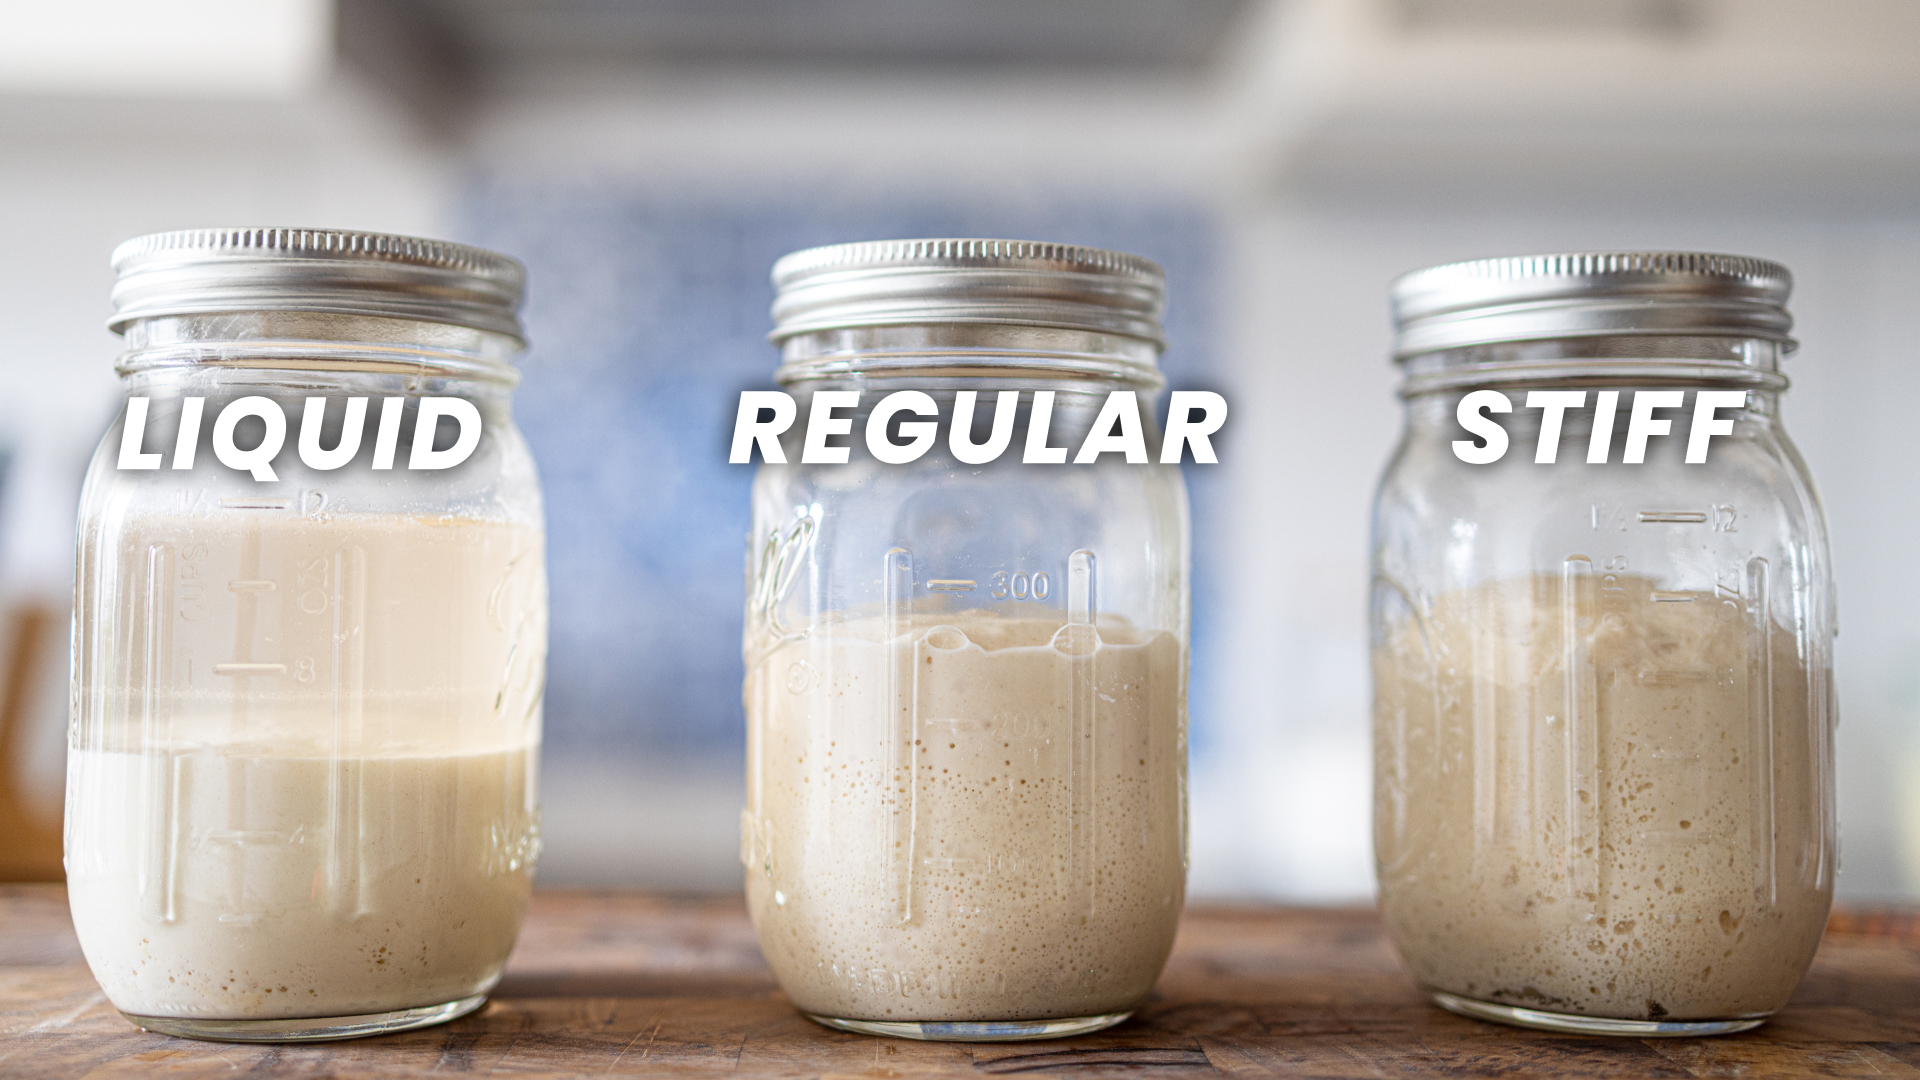
\includegraphics[width=\textwidth]{sourdough-starter-types}
  \caption{3 different starter types next to each other. Note how the liquid starter is submerged
  in water. It has a hydration of 500 percent or more.
  The regular starter has a hydration of around 100 percent, the stiff starter around 50 to 60 percent.}
  \label{fig:starter-types}
\end{figure}


You can change your starter type by just adjusting the feeding ratio of how
much flour and water you use. I frequently change my starter type from
regular to liquid and then back to a stiff starter. After changing the
environment of your microbes, apply feedings at the same ratio over a couple of
days so that they can adapt to the new environment. I typically see
changes after a single feeding, but I recommend 2 to 3 feedings, one feeding per
day, to see a stronger effect.

Your dough is generally just a big sourdough starter. So your starter is going
to adapt and regrow inside of your main dough. But you can influence the
properties that your starter carries over to your main dough. If you have more
bacterial fermentation, then your dough will also have slightly more bacterial
fermentation. If you have more yeast fermentation, then your main dough will
have slightly more yeast fermentation. This is important to know when you are
working with a more mature unfed starter. Let's say your starter had last been
fed 48 hours ago. Chances are that your bacteria is very active while the
yeast could be dormant. In such a case you can skip feeding your starter
before making another dough. Just use a very tiny amount of starter. For 1000 g
of flour I would take around 10 g of starter (1 percent in terms of baker's
math). If my starter is very young and had just been fed 6 to 8 hours ago I might
end up going up to 20 percent of starter. Remember that your dough is nothing
else other than a big starter. It will tremendously help you to figure out
your best next steps.

When using such a low inoculation rate (1 percent), you need to use stronger
flour when making wheat-based doughs. Your flour naturally breaks down due
to enzymatic activity. It might take 24 hours for the starter to re-grow
inside of your bread dough. At the same time, the enzymatic activity might
have caused your gluten to degrade significantly. While this is okay
when looking at your starter, your wheat-based dough will flatten
out during baking and no longer have the typical characteristics (fluffy crumb
structure). A stronger flour with more gluten is thus advised. It allows for
a longer fermentation before most gluten is broken down.

\section{Regular starter}

\begin{figure}[!htb]
  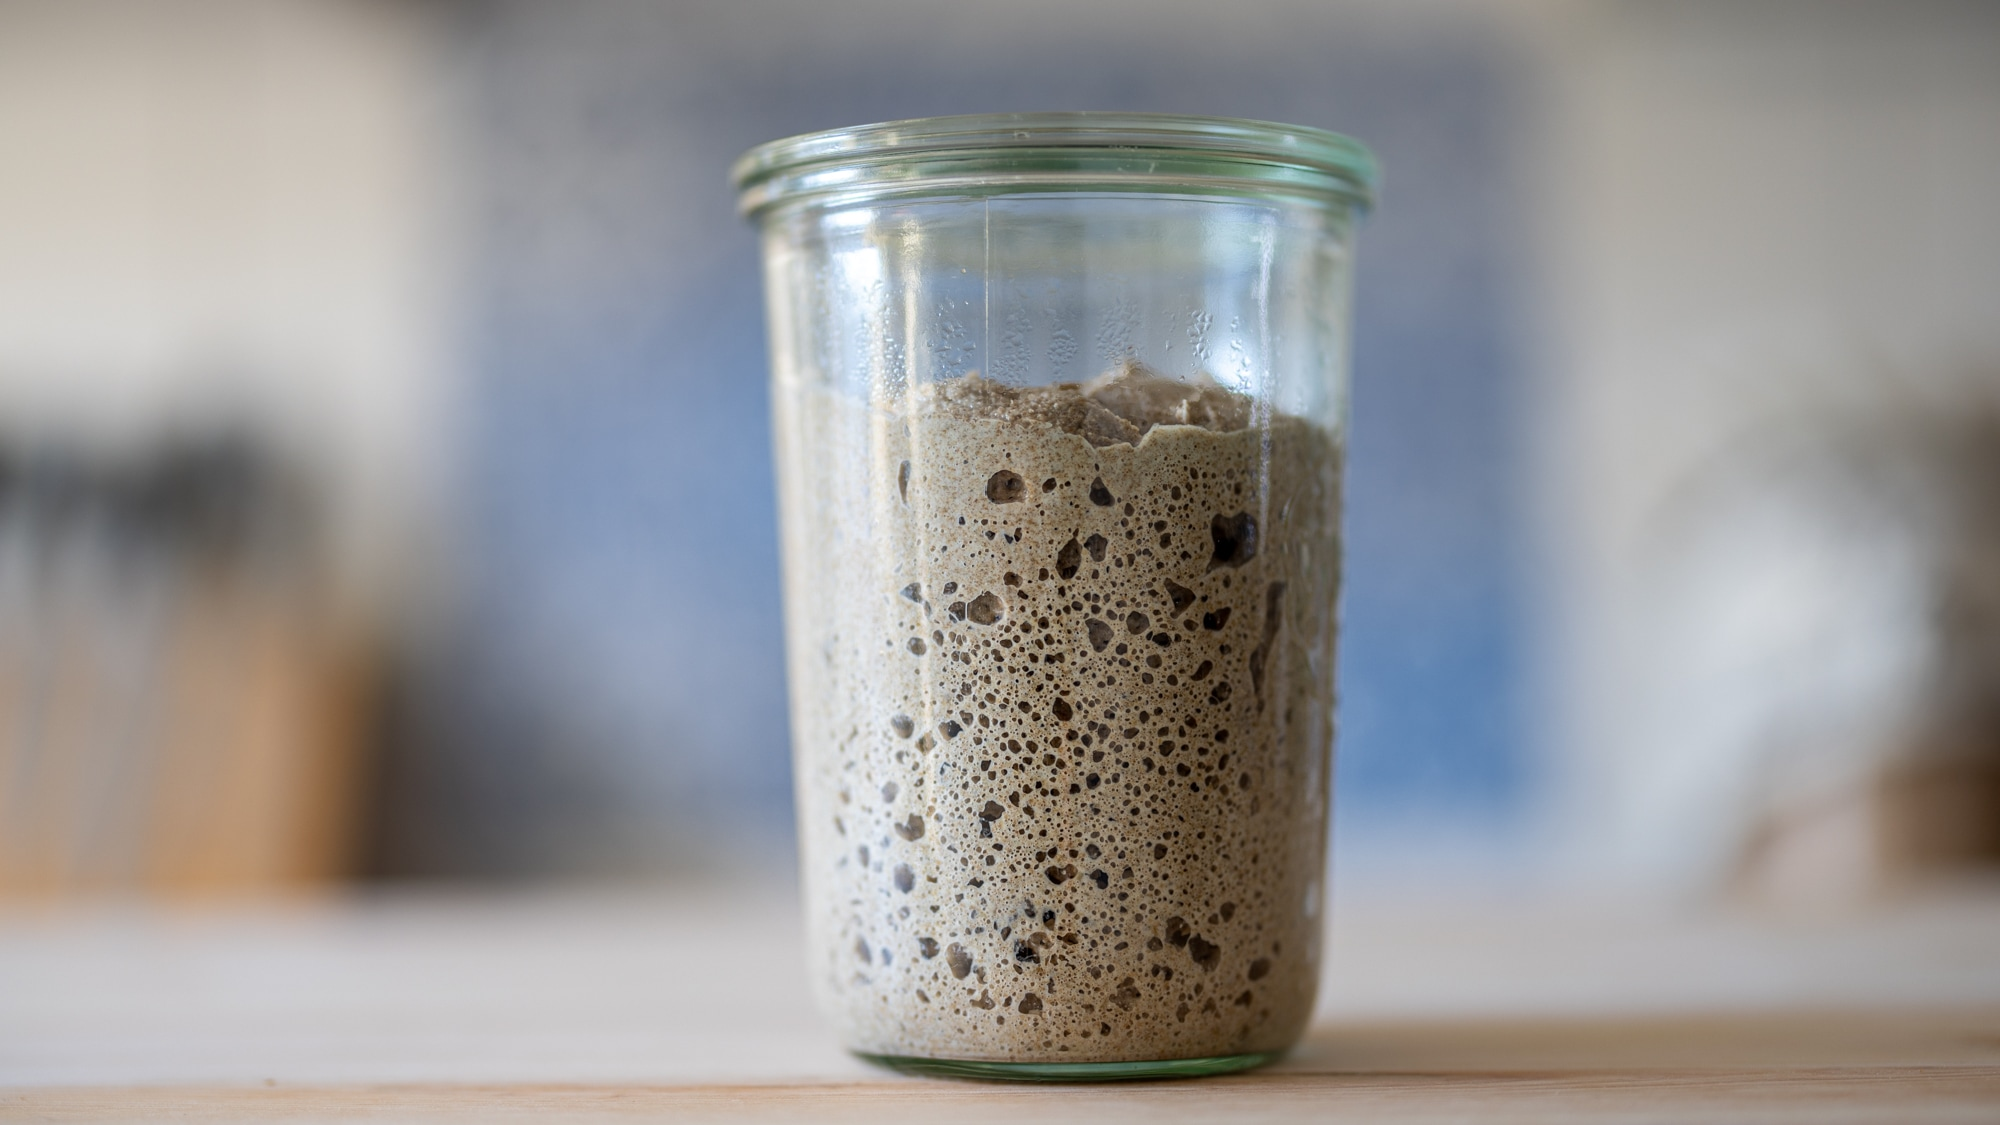
\includegraphics[width=\textwidth]{sourdough-starter.jpg}
  \caption{A regular sourdough starter at 100 percent hydration fed with rye flour}
  \label{fig:regular-sourdough-starter}
\end{figure}

The regular sourdough starter is made at a hydration of around 100 percent.
This means the starter has equal parts of flour and water. This is the most
common and must universal sourdough starter there is. The starter has a good
balance of yeast and bacteria. After a feeding, the volume increases and
increases. After it reaches a certain peak, it will start to collapse again.

The best way to judge whether the starter is ready is to look at signs such as
air pockets on the edges of your container. Also use the nose to evaluate the
smell of your starter. If you feel that the starter doesn't perform in a
desirable way, chances are that your yeast and bacteria ratios are off. In that
case frequent daily feedings using a 1:5:5 (starter:flour:water) ratio will
help.

A regular starter is a perfect choice to use when utilizing stronger wheat or spelt flours.
It also nicely works with rye, emmer or einkorn. If you only have a weak flour
at hand with less gluten, this starter might cause issues. As you tend to have
quite some bacterial activity, gluten is going to be broken down fast. When
using the starter, use around 1 to 20 percent starter based on the flour of your
dough.

Depending on the bacteria cultivated, a regular starter either has a lactic (dairy),
a vinegary (acetic) or mix of both flavor profiles. You can adjust your
starter's flavor by changing the type to a liquid starter.

\section{Liquid starter}
\label{section:liquid-starter}

\begin{figure}[!htb]
  \centering
  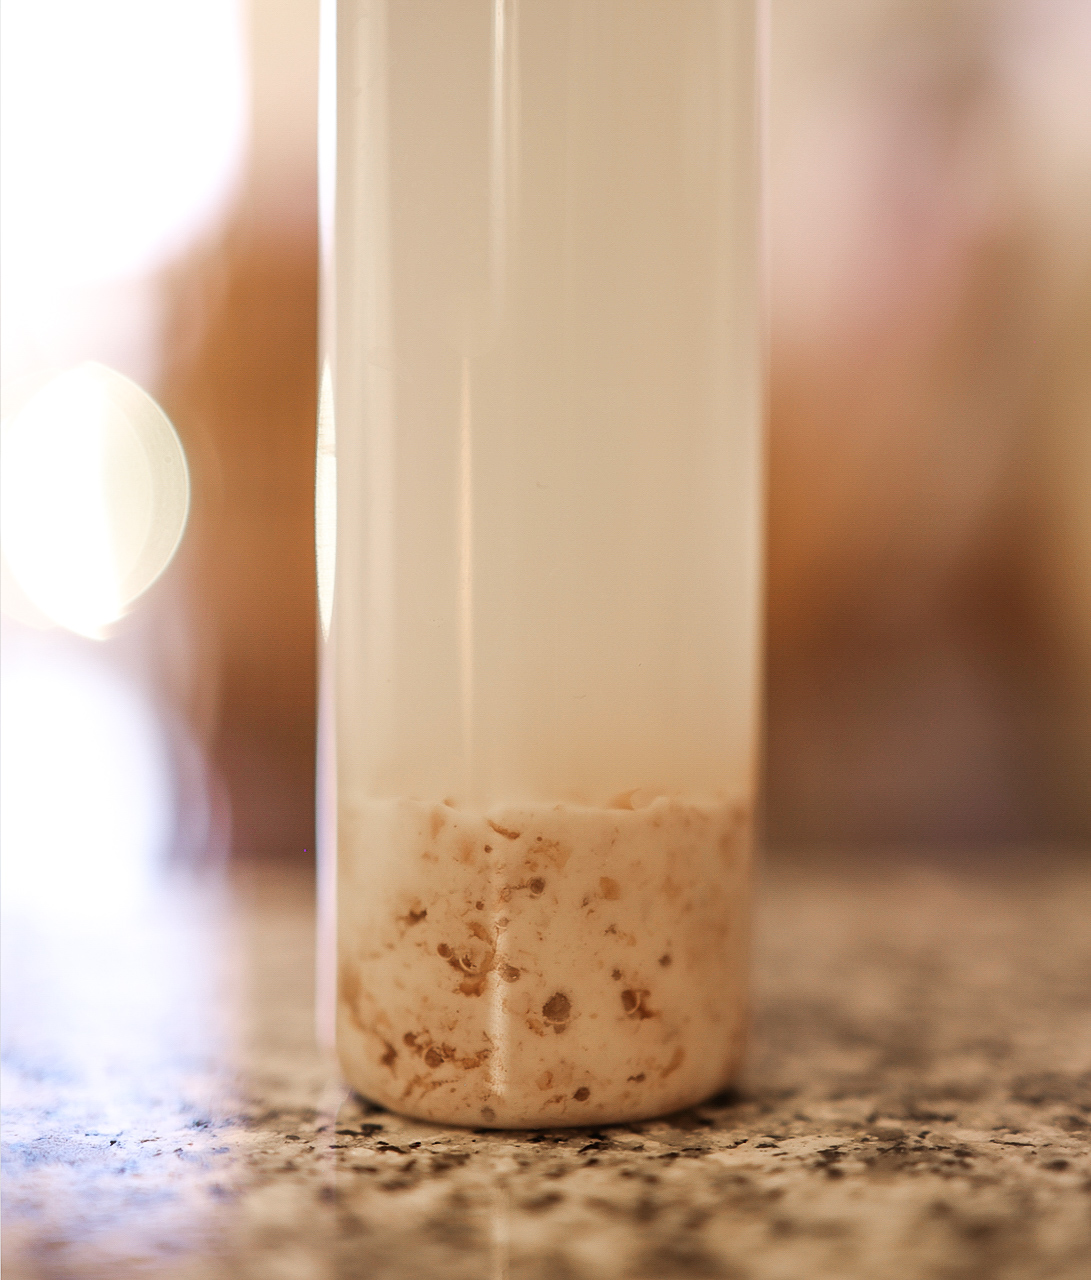
\includegraphics[width=0.5\textwidth]{sourdough-starter-liquid.jpg}
  \caption{A liquid sourdough starter features a high level of water. The high
  water amount boosts lactic acid producing bacteria. After a while the liquid
  and flour start to separate. Bubbles on the side of the flour
  indicate that the starter is ready to be used.}
  \label{fig:liquid-sourdough-starter}
\end{figure}


\begin{figure}[!htb]
  \includegraphics{figures/fig-liquid-starter-conversion.pdf}
  \caption{The process to convert your regular or stiff starter into a liquid starter. The whole
  process takes around 3 days. The longer you maintain your starter at the
  suggested hydration level, the more adapted your microorganisms become. It is recommended
  to keep a backup of your original starter as the liquid environment will select
  anaerobic microorganisms. This boosts bacteria that create lactic acid rather
  than acetic acid. The resulting acidity will be perceived as milder.}
  \label{fig:liquid-starter-conversion}
\end{figure}

The liquid starter is made at a hydration of around 500 percent. This means
the starter has much more water than flour. The additional layer of water on
top of the flour changes the microbiome of your starter.

By introducing this layer of water, less oxygen is available throughout the
course of fermentation. This means that your starter will no longer be
producing acetic acid. The heterofermentative lactic acid bacteria will thrive
in this environment. This is a neat little trick to change your starter's
flavor profile from vinegary to lactic. Your starter is going to develop
dairy creamy notes. Interestingly, when changing the hydration again, your starter
is going to maintain the liquid starter flavor profile, but then benefit again
from enhanced yeast activity. The liquid starter conversion is non reversible.
So ideally keep a backup of your stiff or regular starter.

To commence with the
conversion, simply take around 1 gram of your starter, mix with 5 g flour and
25 g water. Stir everything together properly. After a few minutes the flour is
going to start settling in at the bottom of your jar. Repeat this process over
a few days. Shake the starter gently to see if you can see tiny \ch{CO2} bubbles
moving in the liquid. This is a good sign that your starter is ready. Use your
nose to smell the starter. It should have a creamy dairy flavor note.

As you have more bacterial activity, this starter works best with a very strong
flour that can withstand a long fermentation period. Using this starter with a
weak wheat flour will not work. If you do not care about baking a freestanding loaf,
then you can easily use this starter together with a loaf pan.
This starter also works great when making a hearty pancake dough. To use it I
shake the starter container until I see all ingredients are homogenized. Then
I use around 5 percent of it in terms of baker's math. So for 1000 g of flour
that's around 50 grams of liquid starter. As it is very liquid you have to
include the 50 grams in your liquid calculation. I typically treat the starter
directly as liquid in the recipes. So if the recipe calls for 600 grams of water
and I use 50 grams of starter, then I would proceed and only use 550 grams of
water.

This type of starter is also an excellent mold combatant. As you are removing
oxygen from the equation, aerobic mold can not properly grow. If your starter
has a mold problem then the liquid conversion could be the remedy. Take a
piece of your starter where you suspect no mold growth. Apply the conversion
as mentioned before. The mold will likely sporulate as it runs out of food.
With each new feeding you are reducing the mold spores. The spores can no
longer reactivate as they can not do so in the anaerobic conditions.

The liquid on top of your starter is an excellent resource that you could use
to make sauces. If you feel you would like to add a little bit of acidity,
drain the liquid part on your starter and use it. I have used it numerous
times to make lacto-fermented hot sauces.

\section{Stiff starter}
\label{section:stiff-starter}

\begin{figure}[!htb]
  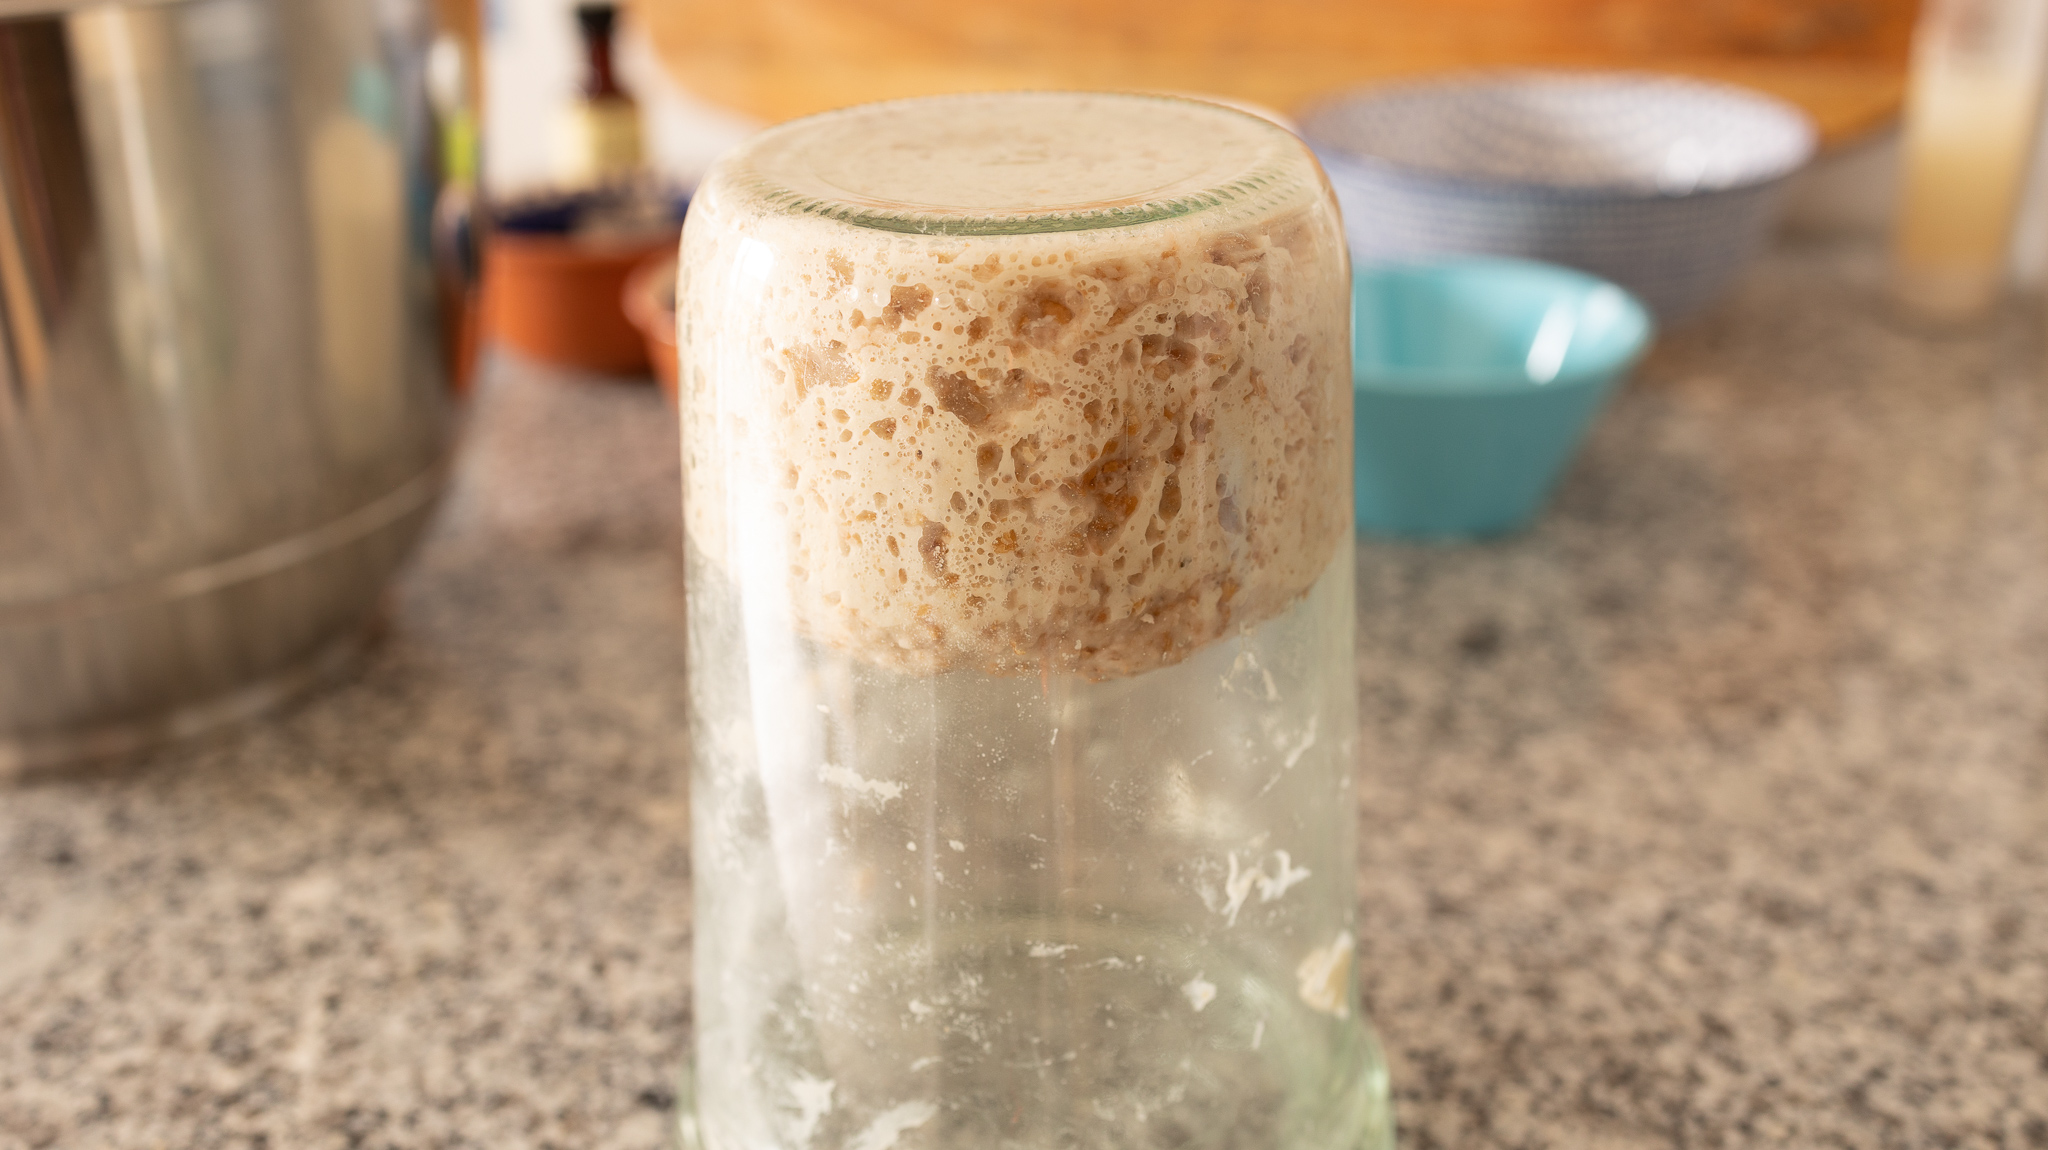
\includegraphics[width=\textwidth]{sourdough-starter-stiff.jpg}
  \caption{A stiff sourdough starter that I used to make a Stollen dough for Christmas. Note
  the bubbles on the edge of the container. The dough does not fall out of the jar.}
  \label{fig:stiff-sourdough-starter}
\end{figure}

The stiff starter is the driest of all the starters. It has a hydration of
around 50 to 60 percent. So for 100 grams of flour you are using around 50 to
60 grams of water.

\begin{figure}[!htb]
  \includegraphics{figures/fig-stiff-starter-conversion.pdf}
  \caption{The process to convert your regular starter into a stiff starter. The whole
  process takes around 3 days. The longer you maintain your starter at the
  suggested hydration level, the more adapted your microorganisms become. The
  stiff starter boosts the yeast activity of your sourdough starter.
  The guide uses a 50 percent hydration level for the starter. If the dough is too stiff
  consider increasing this to 60 percent.}
  \label{fig:stiff-starter-conversion}
\end{figure}

In the stiffer environment the yeast thrives more. This means you will have
more \ch{CO2} production and less acid production. In my tests this is a game
changer especially if you are using weaker gluten flours. The wheat flours in
my home country of Germany tend to be lower in gluten. For wheat to build gluten, warm conditions
are preferred (SOURCE NEEDED). When following recipes from other bakers, I
could never achieve similar results. When following timings my doughs would
simply collapse and become super sticky. Only when I started to buy more
expensive wheat flour did my results start to change. As not everyone can afford
these special baking flours and due to their limited availability, I stumbled upon the
stiff sourdough starter. I made several tests where I used the same amount of
starter and flour. I only changed the hydration between all the starters. I
would then proceed and place a balloon on top of each of the jars. The stiff
starter jar was clearly inflated the most. The regular starter
followed in second place. The liquid starter finished in third place with far less \ch{CO2}
production.

\begin{figure}[!htb]
  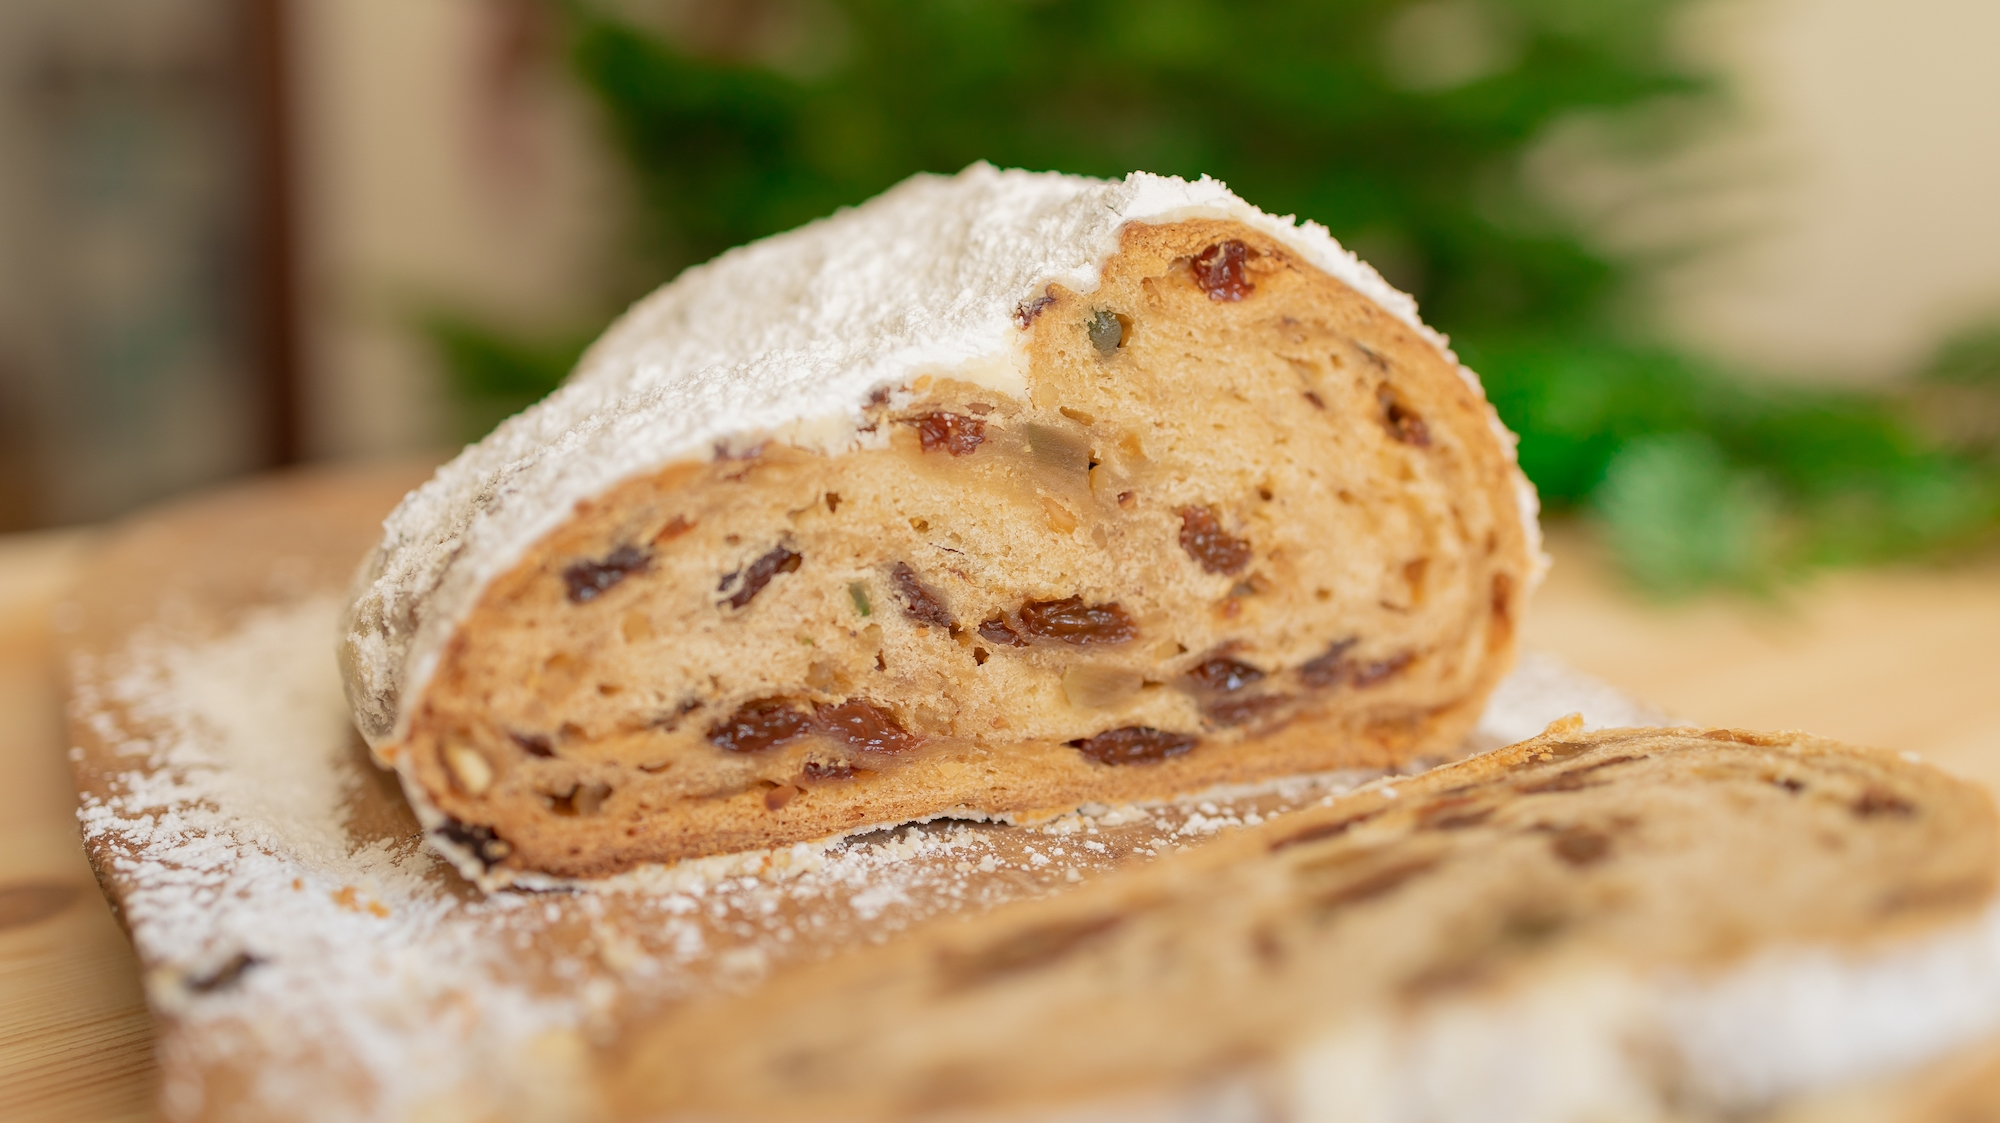
\includegraphics[width=\textwidth]{stollen}
  \caption{A German Christmas stollen made with a stiff starter instead of yeast}
  \label{fig:stollen}
\end{figure}

I then proceeded and bought a cheap low cake flour in my nearby supermarket.
This flour before had caused me massive headaches before. I made a sourdough bread
exactly how I would normally do. I had to reduce the hydration a bit as a low
gluten flour does not soak up as much water. Then I replaced the starter with
the stiff starter. The dough felt amazing and was suddenly able to withstand a
much longer fermentation period. The bread had great oven spring and tasted
very mild. I am still yet to find a proper explanation why the yeast part of
the dough is more active. Maybe it is not. It could also be that the bacteria
is inhibited by the lack of water.

When making the stiff sourdough starter, start by using around 50 percent
water. If you are using a whole wheat flour, or a strong flour consider going
up to 60 percent. All the ingredients should mix together very well. There
should be no crumbly flour left. This is a common mistake I have seen when
people tried to make the stiff starter. Yes it should be dry, but not to a
point where it is a brick of cement. If you have ever made a pasta dough, this
dough should exactly feel the same.

To evaluate whether your stiff starter is ready, look for a dome. Also look for
pockets of air on the sides of your container. Use your nose to smell the
starter. It should have a mild smell. It also tends to smell much more
alcoholic than the other starters.

When using a stiff starter, use around 1 to 20 percent depending on the ripeness of
your starter. In summer I typically use around 10 percent and in winter
around 20 percent. This way you can also control the fermentation speed.
Mixing the starter can be a little bit annoying as it hardly homogenizes with
the rest of the dough. In this case you can try to dissolve the starter in the
water you are about to use for your dough. This will make mixing a lot easier.


\section{Lievito madre or pasta madre}

The lievito madre, also known as pasta madre, belongs to the same category as
the stiff sourdough starter. After conducting hours of research, I could not
find a difference in pasta madre and lievito madre. Both terms seem to be
used interchangeably in literature.

In many recipes this starter is made directly
from dried or fresh fruits. You can also make a starter from leaves from your
garden. As described before, the wild yeast and bacteria consume the glucose
from the plants' leaves. All the options work. When making a starter directly
from dried fruits, you sometimes lack the bacterial part of the fermentation.
The acidity is very important in order to clean your starter from possible
pathogens. If you decide to make your starter from fruits, make sure it also
acidifies properly when making a dough. A tool such as a pH meter can be of
optimal help. Generally, the lower the pH, the higher the acidity. The acidity
should be below 4.2 to know that your starter produces sufficient acidity.

Some bakers cleanse the lievito madre in a bath of water. This is supposed to
remove excess acidity. In my own experiments I have not been able to confirm
this methodology. The acidity remains the same. The only reason this could
make sense is if you also tried to boost anaerobic microorganisms. However, then the
starter would need to remain in this environment for quite some time and not just
a few hours.

Baking with sourdough is simple. It's just flour and water. When seeing a recipe
from an experienced baker you wonder, Wait, that's it? There is nothing more
to it? I feel that this might be the reason why some bakers have such complicated
feeding procedures. They resort to several feedings per day at a certain given ratio.
This makes the baker feel a little more elitist. Of course over time as
more and more people follow this procedure, it becomes a self fulfilling prophecy.
The more experienced you become, the higher the chances are that a bogus starter
feeding guide will reward you with beautiful results. The reason however is
not in the starter routine. The reason is that you understand the fermentation better
and become better at reading the signs of your dough.

If I had to choose one starter type I would go for the stiff starter. In many cases
it will provide you with consistently great results with little effort.
In my experience you can make any yeast-based dough and just replace
the yeast directly with the stiff sourdough starter. You will be able
to achieve even better results with the stiff starter.

Lastly, no matter which starter type you choose, you can control how sour
you want your dough to be. The longer you push the fermentation, the more
acidity is going to be piled up. The only difference is that for a given
volume increase, the stiff starter will produce the least acidity. So for a
volume increase of 100 percent, the liquid starter has produced the most acidity,
followed by the regular starter and then the stiff starter. If you wait long
enough, the stiff starter will have produced the same amount of acidity as the
other starters. But before doing so it will have also produced a lot more \ch{CO2}. If
you like the sour flavor, you have to push your fermentation longer. This also
means you either need to bake in a loaf pan or have a very strong gluten flour
that is able to withstand long fermentation times.


\chapter{Flour types}
\begin{quoting}
In this chapter we will have a closer look at different flour types
and their respective categorization. We will also look at common
ways to distinguish different flours of the same type. This way you can more confidently
purchase the flour that you need.
\end{quoting}

The most basic flour type is a whole grain flour. In this case the whole seed has
been grounded to smaller pieces. Sometimes, depending on what you want to bake,
the hearty taste of the bran might not be desired. In this case you can use
whiter flours. With sieves, mills remove larger parts of the hull of the seed.
The seed already contains a pre-built germ from the plant waiting to be
activated. The whitest flour you can get is mostly just the starch part of the seed.
Depending on which layers are still present, names are used to describe the
type of flour.

\begin{table}[!htb]
    \begin{center}
        \begin{tabular}{@{}llrrr@{}}
\toprule
\textbf{USA}  & \textbf{UK}  & {\textbf{Germany}} & {\textbf{France}} & {\textbf{Italy}} \\ \midrule
Cake         & Soft flour  &  T405    &  T45   & 00 \\ 
All purpose  & Plain flour &  T550    &  T55   &  0 \\ 
             &             &  T812    &  T80   &  1 \\ 
             &             & T1050    & T110   &  2 \\ 
Whole        & Whole       & Vollkorn & T150   & Integrale \\ \bottomrule
\end{tabular}

        \caption[Labelling of wheat flour]{A comparison of how different types
            of wheat flour are labelled in different countries.}%
        \label{tab:flour-types-comparison}
    \end{center}
\end{table}

In Germany, the ash content is used to describe the flours. The lab will burn
\qty{100}{\gram} of flour in the oven. Then afterwards the remaining ash is extracted
and measured. Depending on the quantity the flour is categorized. If the flour
is of type 405 then \qty{405}{\mg} of ash have remained after burning the
flour. The more hull parts the flour has, the more minerals remain. So the
higher the number, the closer the flour is to whole flour. The numbers are
slightly different between each grain type. Generally though, the higher the
value, the heartier the taste is going to be.

\begin{figure}[htb!]
  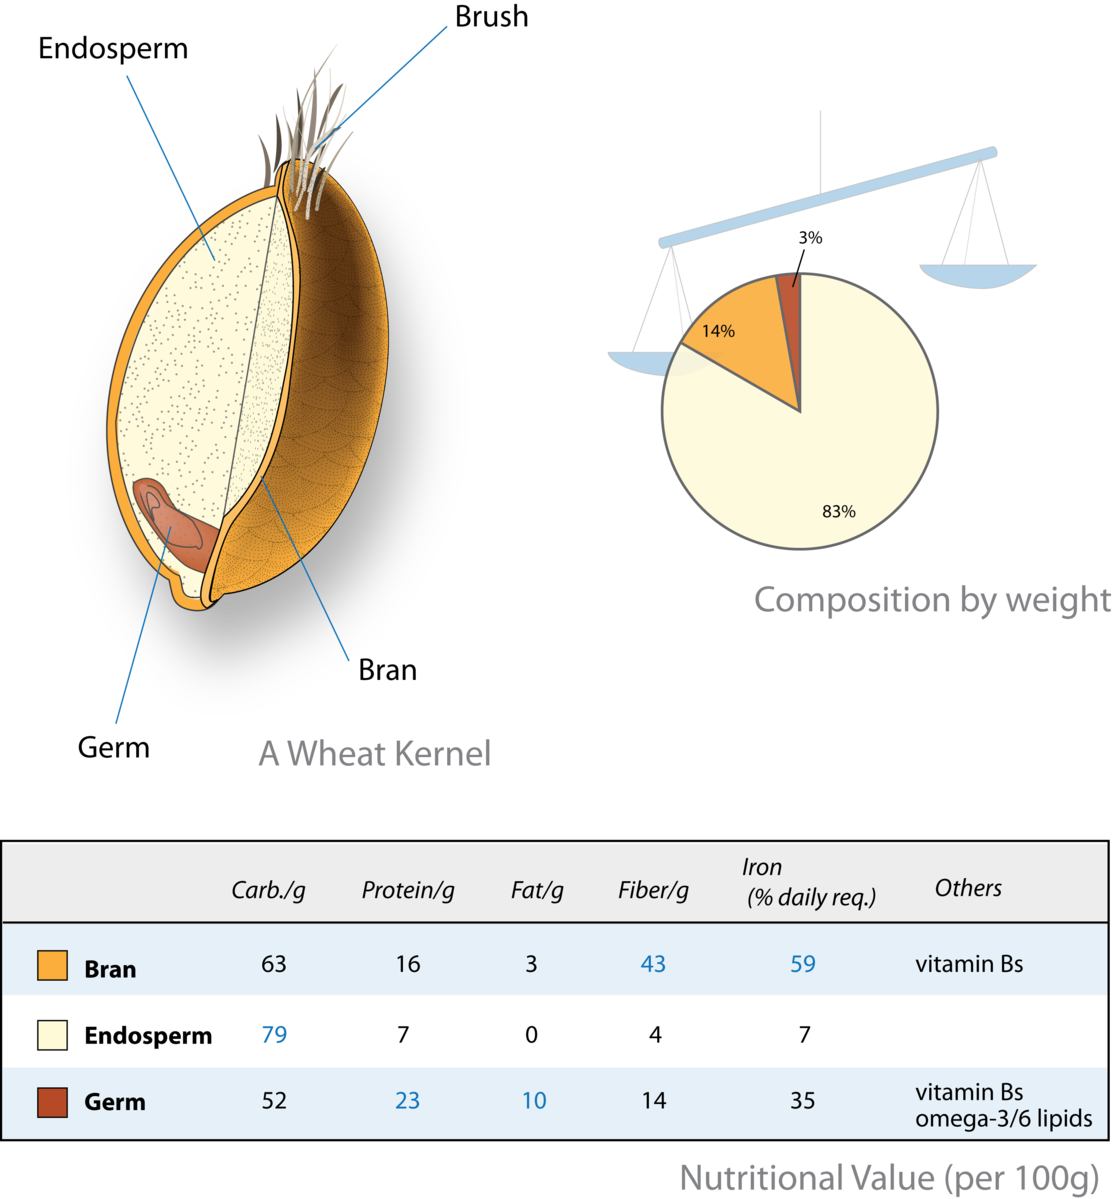
\includegraphics[width=\textwidth]{wheat-kernel-overview}
  \caption[Content of a wheat kernel]{An overview of a wheat kernel together
      with its content~\cite{wheat+kernel}.}%
  \label{fig:wheat-kernel-overview}
\end{figure}

If you compare different grain types, there are grains with high gluten, low gluten
and no gluten. Gluten is what enables bread to have its fluffy consistency.
Without gluten the baked goods wouldn't have the same properties. Managing
gluten makes the whole bread-making process more complex as more steps are involved.
A dough without gluten doesn't have to be kneaded. Kneading creates
the gluten bonds. The more you knead, the stronger they become. With low-gluten
and no-gluten flours, you only have to mix the ingredients together, making
sure you properly homogenize everything. During fermentation
the gluten degrades as the microorganisms metabolize it. When too much gluten
has been converted your dough will no longer have the wheat-like structure previously
described. For no/low gluten flour your main focus is managing acidity. You do not
want the final bread to be too sour. You do not have to worry about the gluten
degradation, removing a huge headache from the equation.

\begin{table}[!htb]
    \begin{center}
        \documentclass[tikz]{standalone}
\usepackage{tikz}
\usepackage{siunitx}
\DeclareSIUnit\degF{\text{°}F}

\begin{document}
\begin{tabular}{|l|l|l|l|l|}
\hline
\textbf{Grain type}              & \textbf{Homogenize} & \textbf{Knead} & \textbf{Stretch \& Fold} & \textbf{Shape} \\ \hline
\textbf{Wheat}                   & Yes                 & Yes            & Yes                      & Yes            \\ \hline
\textbf{\textgreater 70\% Wheat} & Yes                 & Yes            & Yes                      & Yes            \\ \hline
\textbf{Spelt}                   & Yes                 & Yes            & Yes                      & Yes            \\ \hline
\textbf{Rye}                     & Yes                 & No             & No                       & No             \\ \hline
\textbf{Emmer}                   & Yes                 & No             & No                       & No             \\ \hline
\textbf{Einkorn}                 & Yes                 & No             & No                       & No             \\ \hline
\textbf{Rice}                    & Yes                 & No             & No                       & No             \\ \hline
\textbf{Corn}                    & Yes                 & No             & No                       & No             \\ \hline
\end{tabular}
\end{document}

        \caption[Different types of grain]{An overview of different grain
          types and the steps involved in the respective bread making process.}
    \end{center}
\end{table}

As gluten has a special role, the rest of this chapter is dedicated to having a
closer look at different gluten flours and how to distinguish them. Spelt
also contains significant amounts of gluten, so the same characteristics hold
true.

Several recipes call for wheat bread flour. Bread flour can refer to different types
of flour. It could be a T405 or a T550 in Germany. This is very often
classified incorrectly. The terms \emph{strong} or \emph{bread} flour in this case
refer to the properties of the flour. A bread flour is considered to have a
higher amount of protein and thus gluten. This flour is excellent when you
want to make a sourdough bread as your dough allows for a longer leavening
period. As described earlier, the gluten is consumed by your microorganisms.
The more gluten you have, the longer your dough keeps its integrity. If you wanted
to make a cake, you might want to use a flour with less gluten. The gluten binding
properties might not be desirable since the final cake could have a chewy texture.

In conclusion, not every T405, T45 or T00 flour is the same. Depending on the properties
of the plant they come from, the flours will have different properties. For that reason
some countries like Germany have introduced additional scales to evaluate the quality of the
wheat. The category \textbf{A} refers to good quality wheat that can be blended
with poorer qualities to improve the flour. The category \textbf{B} refers to
average wheat that can be used to create different baked goods. Category \textbf{C}
is used for wheat that has poor baking qualities. This could happen, for instance,
if the wheat already started to sprout and thus lost some of its desirable
baking properties. This type of wheat is typically used in animal feed or
as fermentable biomass for generators. Category \textbf{E} refers to \emph{Elite} wheat. It's
the highest quality of wheat. This kind of wheat can only be harvested when the
wheat has grown under optimal conditions. You can compare this to a winery
that uses only the best grapes to make a reserve wine. Unfortunately, this is normally never printed
on the packaging of the flour that you buy. You can look out for the protein
value as a possible indicator. However, large mills blend flours together to
maintain quality throughout the years. Blended flour is also not listed on
the packaging. It might be that bakeries extract gluten from some flour and
then mix it in order to create better baking flours.

In Italy the so-called
\textbf{W-value} has been introduced to better show how the flour will behave.
A dough is made, and then the resistance of this dough to kneading is measured.
The more gluten a flour has, the more elastic the dough is, and the more it will
resist kneading. A higher W flour will have a higher gluten content and allow for a longer
fermentation period. But at the same time, it is also harder for the microbes to
inflate the dough as there is more balloon material. To make an excellent fermented
product out of a high W flour you will need to have a long fermentation period.
The long fermentation period also means that your microbes will enrich
your dough with more flavor.

\begin{table}[!htb]
    \begin{center}
        \begin{tabular}{@{}rcll@{}}
\toprule
\textbf{W-Value} & \textbf{Hydration (\%)} & \textbf{Uses} & \textbf{Fermentation time} \\ \midrule
0--150          & 50     & Cookies             & Very short    \\ 
150--250        & 50--60 & Cakes, Bread, Pizza & Short--Medium \\ 
250--350        & 60--70 & Bread, Pizza        & Long          \\ 
350+            & 70--90 & Bread, Pizza        & Very long     \\ \bottomrule
\end{tabular}

        \caption[Fermentation time versus W-value]{An overview of different
            levels of W-values and the respective hydrations and fermentation
            times.}%
        \label{tab:w-value}
    \end{center}
\end{table}

Generally, when aiming to
bake free standing sourdough bread, aim for a higher protein content. If the
gluten value is relatively low, your bread will collapse faster. Baking bread
is still possible, but it might be easier to use tools such as a loaf pan, or
to make skilled bread or flatbread.

An additional, rarely considered characteristic of good flour is the level of damage to the
starch molecules. This is a common problem when you are trying to mill your own wheat flours at
home. The chances are that your home mill is not able to achieve the same results
a larger mill can. The damaging of the starches is essential to improve the
properties of the dough. You will have better gelatinization and water
absorption with properly damaged starch~\cite{starch+damage+flour}. As more
starch is damaged, the surface area increases. This improves how water interacts with the flour.
This also provides a larger surface that your microbes can use to attack the molecules
and start the fermentation process.

I~am still
yet to find a good way of milling my own flour at home. Even after trying to
mill the flour 10 times with short breaks, I~was not able to achieve the same
properties as with commercially milled flour. The doughs I~would make felt
good, maybe a bit coarse. However, during baking the doughs would start to
de-gas quickly and turn into very flat breads. I~have had great success though when
utilizing home-milled flour together with a loaf pan or as a pan bread. If you
have found great ways to work with home-milled flour, please reach out. The potential
of using home-milled flours is huge. It would enable even distant communities
to grow their own wheat and be able to produce amazing freshly baked bread.


\chapter{Bread types}
\section{Wheat bread basics}
\section{Non wheat bread basics}
\section{The simplest way to make bread}

\chapter{Wheat sourdough}
\section{The process}
\section{Readying your starter}
\section{Ingredients}
\section{Hydration}
\section{Autolyse}
\section{Fermentolyse}
\section{Dough strength}
\section{Controlling fermentation}
\section{Optional Preshaping}
\section{Shaping}
\section{Proofing}

\chapter{Non wheat bread basics}
\section{Ingredients}
\section{Managing acidity}
\section{To shape or not to shape}
\section{Proofing}

\chapter{Baking}
\section{The role of steam}
\section{Temperature}
\section{Home oven setup}
\section{Dutch ovens}

\chapter{Storing bread}
\section{Fridge}
\section{Room temperature}
\section{Frozen}

\chapter{Troubleshooting}

\section{Debugging your crumb structure}%
\label{section:debugging-crumb-structure}

The crumb structure of your bread provides insights into how well
your fermentation process has gone. You can also spot common flaws
arising from improper technique. This chapter will provide you with information
that you can use to debug your baking process.

\begin{figure}
  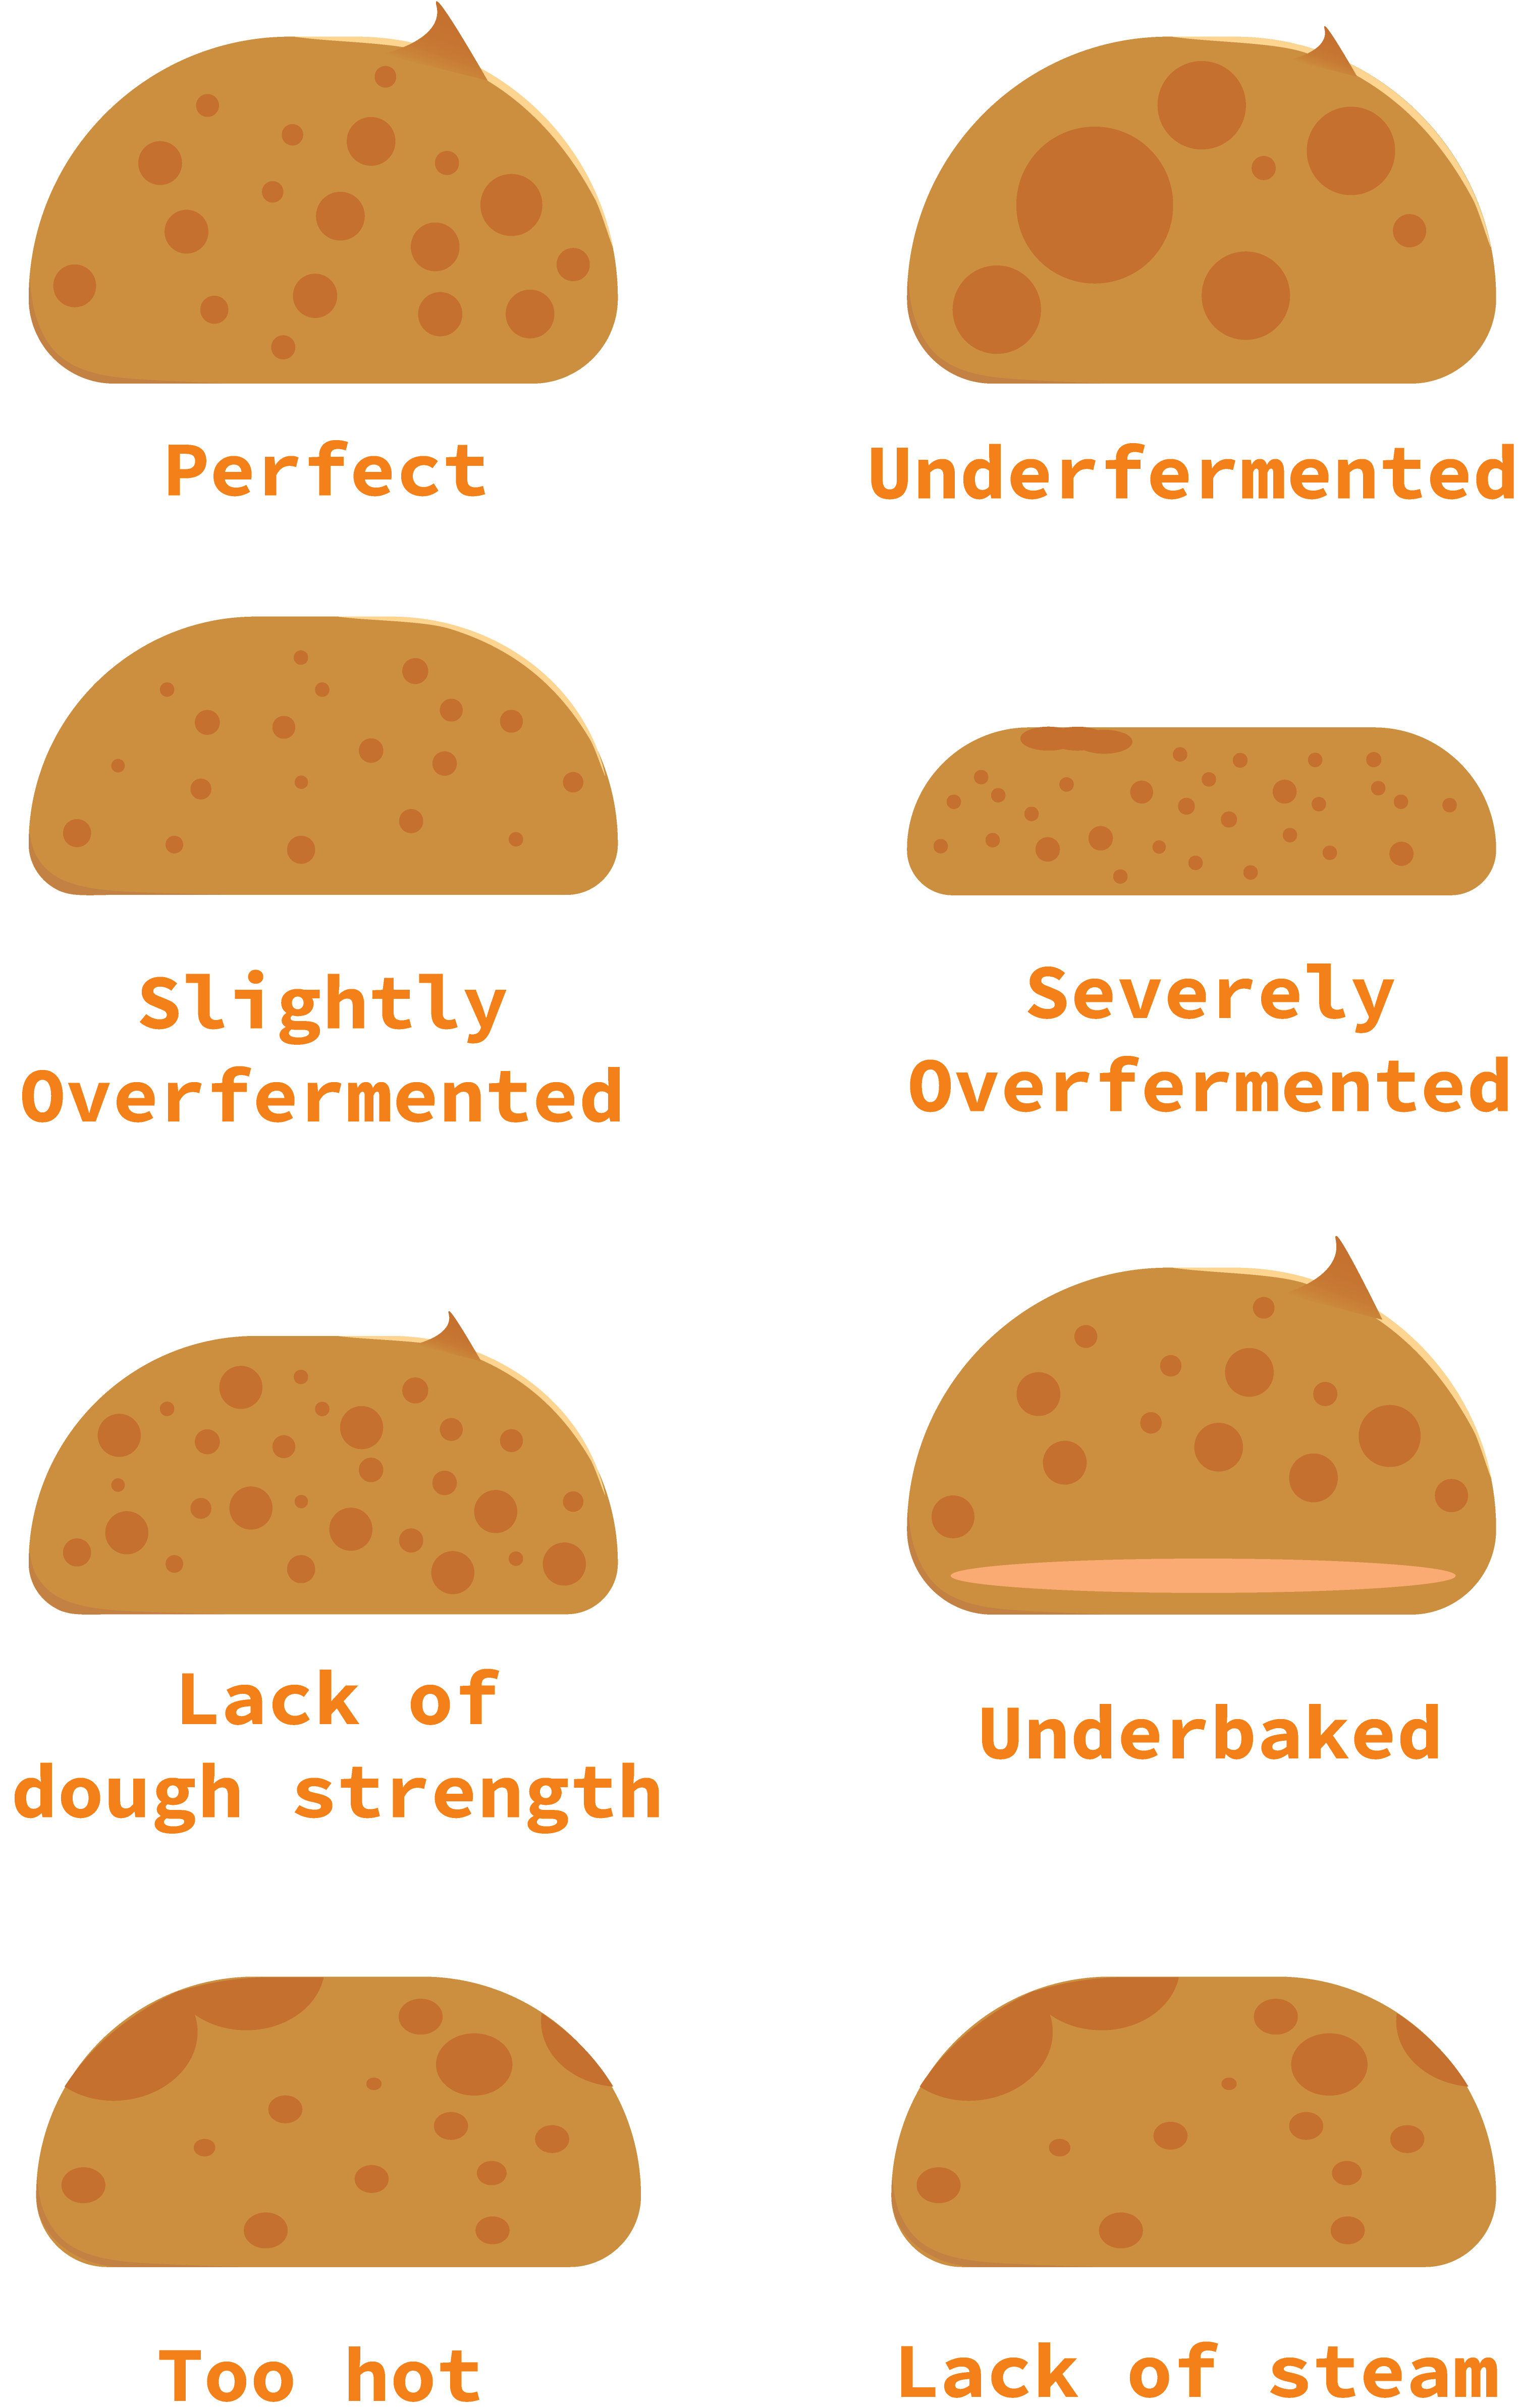
\includegraphics[width=\textwidth]{crumb-structures-book}
  \caption{A schematic visualization of different crumb structures and their respective causes. The
  final bread's crumb is a key aspect to identify potential issues related to fermentation
  or baking technique.}%
  \label{fig:crumb-structures-book}
\end{figure}

\subsection{Perfect fermentation}=

\begin{figure}
  \includegraphics[width=\textwidth]{open-crumb}
  \caption{The bread has a somewhat open crumb with areas
  featuring a honeycomb structure.}%
  \label{fig:open-crumb}
\end{figure}

Of course the perfect fermentation is debatable and highly subjective. To
me the perfect sourdough bread features a crisp crust paired with a fluffy,
somewhat open crumb. This is the perfect balance of different consistencies
when you take a bite.

Some people are chasers of a very open crumb, meaning you have large pockets
of air (alveoli). It's subjective whether that's the style of bread that you like;
however, to achieve it you need to ferment your bread dough perfectly.
It takes a lot of skill both in terms of mastering fermentation and technique
to achieve a crumb structure like that.

Personally, I~like a bread like that, just with a slightly less wild crumb.
The style of crumb I~like is called the \emph{honeycomb crumb}. It's not too open, but
just enough open to make the bread very fluffy. To achieve the previously mentioned open crumb, you
have to touch your dough as little as possible. The more you interact with your
dough, the more you are degassing your dough. Excess touching of the dough
results in the dough's alveoli merging together. The crumb will not be as open.
That's why achieving such a crumb works best if you only ferment
one loaf at a time. Normally, if you have to pre-shape your dough,
you will automatically degas your dough a little bit during the rounding process.
If you skip this step and directly shape your dough, you will achieve a more open crumb.
A good rule of thumb is to not touch your dough for at least 1--2 hours before shaping,
to achieve as open a crumb as possible.

\begin{figure}
  \includegraphics[width=\textwidth]{honeycomb}
  \caption{A whole wheat sourdough with an almost exclusive honeycomb crumb
  structure.}%
  \label{fig:honeycomb}
\end{figure}


Now this is problematic when you want to
make multiple loaves at the same time. Pre-shaping is essential as you are required
to divide your large bulk dough into smaller chunks. Without the pre-shaping
process, you would end up with many non-uniform bread doughs. This technique is
also used when making ciabattas. They are typically not shaped. You only cut the
bulk dough into smaller pieces, trying to work the dough as little as possible.
With pre-shaping you will converge your dough's alveoli into more of a honeycomb structure,
as large pockets of air will slightly merge. Similarly to the open crumb structure,
you also have to nail the fermentation process perfectly to achieve this crumb.
Too long a fermentation will result in gas leaking out of your dough while baking.
The honeycombs won't be able to retain the gas. If you ferment for too short a time,
there is not enough gas to inflate the structures. To me this is the perfect
style of crumb. As someone who appreciates jam, no jam will fall through a slice
of this bread compared to an open crumb.

\subsection{Overfermented}%
\label{sec:overfermented-dough}

\begin{figure}
  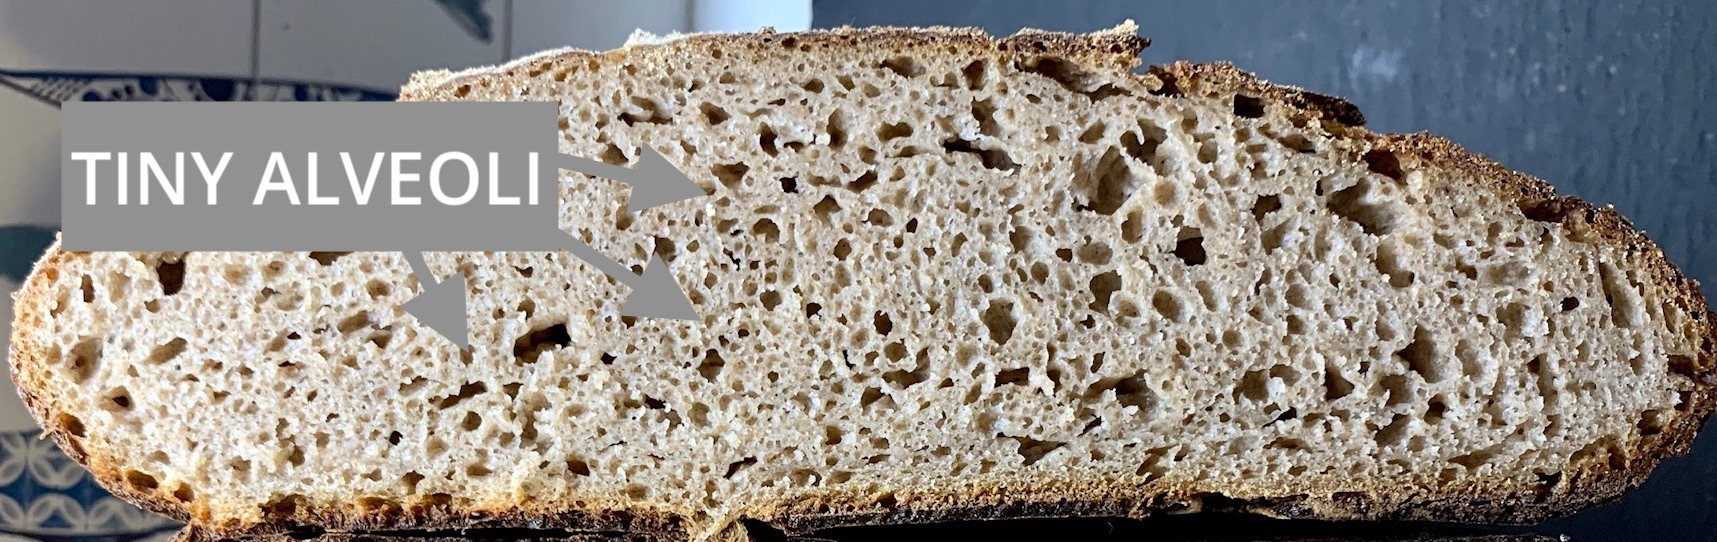
\includegraphics[width=\textwidth]{fermented-too-long}
  \caption{A relatively flat dough that has many tiny pockets of air.}%
  \label{fig:fermented-too-long}
\end{figure}

When fermenting your dough for too long, the protease enzyme starts to
break down the gluten of your flour. Furthermore, the bacteria consume the gluten
in a process called \emph{proteolysis}~\cite{raffaella+di+cagno}.
Bakers also refer to this process as \emph{gluten rot}.
The gluten that normally traps the \ch{CO2} created
by the fermentation process of your microorganisms can no longer keep the
gas inside of the dough. The gas disperses outward resulting in smaller alveoli in your crumb.
The bread itself tends to be very flat in the oven. Bakers often refer
to this style of bread as a \emph{pancake}. The oven spring can be compared
to bread doughs made out of low-gluten flour like einkorn.

Your bread will feature a lot of acidity, a really strong distinctive tang. From
a taste perspective, it might be a little bit too sour. From my own tests with family and
friends (n=15--20), I~can say that this style of bread is typically
appreciated less. However, I~personally really like the hearty strong taste.
It is excellent in combination with something
sweet or a soup.  From a consistency perspective, it is no longer as fluffy as it could be.
The crumb might also taste a little bit gummy. That's because it has been broken down a lot
by the bacteria. Furthermore, this style of bread has a significantly lower amount of gluten~\cite{raffaella+di+cagno}
and is no longer comparable to raw flour, it's a fully fermented product.
You can compare it with a blue cheese that is almost lactose free.

When trying to work with the dough, you will notice that suddenly the dough feels
very sticky. You can no longer properly shape and work the dough. When trying to
remove the dough from a banneton, the dough flattens out a lot. Furthermore,
in many cases your dough might stick to the banneton. When beginning with baking
I~would use a lot of rice flour in my banneton to dry out the surface of the dough a lot.
This way the dough wouldn't stick, despite being overfermented. However as it
turns out the stickiness issue has been my lack of understanding the fermentation
process. Now I~never use rice flour, except when trying to apply decorative scorings.
Properly managing fermentation results in a dough that is not sticky.

If you are noticing, during a stretch and fold or during shaping, that your dough
is suddenly overly sticky, then the best option is to use a loaf pan. Simply take
your dough and toss it into a loaf pan. Wait until the dough mixture has increased
in size a bit again and then bake it. You will have a very good-tasting sourdough
bread. If it's a bit too sour, you can just bake your dough for a longer period
of time to boil away some of the acidity during the baking process. You can also use
your dough to set up a new starter and try again tomorrow. Lastly, if you are hungry,
you can simply pour some of your dough directly into a heated pan with a bit of
oil. It will make delicious sourdough flatbreads.

To fix issues related to over-fermentation, you need to stop the fermentation process
earlier. What I~like to do is to extract a small fermentation sample from my dough.
Depending on the volume increase of this sample, I~can mostly judge when my fermentation
is finished. Try to start with a 25 percent volume increase of your main dough or sample.
Depending on how much gluten your flour has, you can ferment for a longer period of time.
With a strong flour featuring a 14--15 percent protein, you should be able to safely
ferment until a 100 percent size increase. This however also depends on your
sourdough starter's composition of yeast and bacteria. The more bacterial fermentation,
the faster your dough structure breaks down. Frequent feedings of your sourdough
starter will improve the yeast activity. Furthermore, a stiff sourdough starter
might be a good solution too. The enhanced yeast activity will result in a more fluffy
dough with less bacterial activity. A better yeast activity also will result
in less acidity in your final bread. If you are a chaser of a very strong tangy
flavor profile, then a stronger flour with more gluten will help.


\subsection{Underfermented}

\begin{figure}
  \includegraphics[width=\textwidth]{fermented-too-short-underbaked}
  \caption{A dense dough featuring a gummy, not fully gelatinized area.
  The picture has been provided by the user wahlfeld from our community
Discord server.}%
  \label{fig:fermented-too-short-underbaked}
\end{figure}

This defect is also commonly referred to as \emph{underproofed}. However underproofed
is not a good term as it only refers to having a short final
proofing stage of the bread-making process.
If you were to bake your bread after a perfectly-timed bulk fermentation stage,
the result will not be underproofed even if you skipped the proofing stage entirely.
Proofing will make your dough a bit more extensible and allows your sourdough
to inflate the dough a bit more. When faced with an underfermented bread, something
went wrong earlier during the bulk fermentation stage, or maybe even
before with your sourdough starter.

A typical underfermented dough has very large pockets of air and is partially
wet and gummy in some areas of the dough. The large pockets can be compared
to making a non-leavened wheat or corn tortilla. As you bake the dough in your pan,
the water slowly starts to evaporate. The gas is trapped in the structure of the dough
and will create pockets. In case of a tortilla, this is the desired behavior.
But when you observe this process in a larger dough, you will create several
super alveoli. The water evaporates, and the first alveoli form. Then at some point,
the starch starts to gelatinize and becomes solid. This happens first inside of the pockets
as the interior heats up faster compared to the rest of the dough. Once all the starch
has gelatinized, the alveoli holds their shape and no longer expand. During this
process other parts of the bread dough are pushed outwards. That's why an underfermented
dough sometimes even features an ear during the baking process. This
is also commonly referred to as a \emph{fool's crumb}. You are excited about an ear which
can be quite hard to achieve. Plus you might think you finally created some big pockets
of air in your crumb. But in reality you fermented for too short a period
of time.

\begin{figure}
  \includegraphics[width=\textwidth]{fools-crumb}
  \caption{A typical example of a fool's crumb featuring an ear and several overly
  large alveoli. The picture has been provided by Rochelle from our
  community Discord server.}%
  \label{fools-crumb}
\end{figure}

In a properly fermented dough, the alveoli help with the heat transfer throughout the dough.
From within the many tiny fermentation-induced pockets, the starch gelatinizes. With
an underfermented dough, this heat transfer does not properly work. Because of that
you sometimes have areas which look like raw dough. Bakers refer to this as a very
gummy structure sometimes. Baking your dough for a longer period of time would also properly
gelatinize the starch in these areas. However, then other parts of your bread
might be baked too long.

To fix issues related to under-fermentation, you simply have to ferment your dough
for a longer period of time. Now, there is an upper limit to fermentation time
as your flour starts to break down the moment it is in contact with water. That's why it
might be a good idea to simply speed up your fermentation process. As a rough
figure, I~try to aim for a bulk fermentation time of around 8--12 hours typically.
To achieve that you can try to make your sourdough starter more active.  This can be done
by feeding your starter daily over several days. Use the same ratio as you would
do for your main bread dough. Assuming you use 20 percent starter calculated on the flour,
use a 1:5:5 ratio to feed your starter. That would be 10 grams of existing starter,
50 grams of flour, 50 grams of water for instance.
To boost your yeast activity even more, you can consider making a stiff sourdough 
starter. The bacteria produces mostly acid. The more acidity
is piled up, the less active your yeast is. The stiff sourdough starter
enables you to start your dough's fermentation with stronger yeast activity
and less bacterial activity.

\subsection{Not enough dough strength}

\begin{figure}
  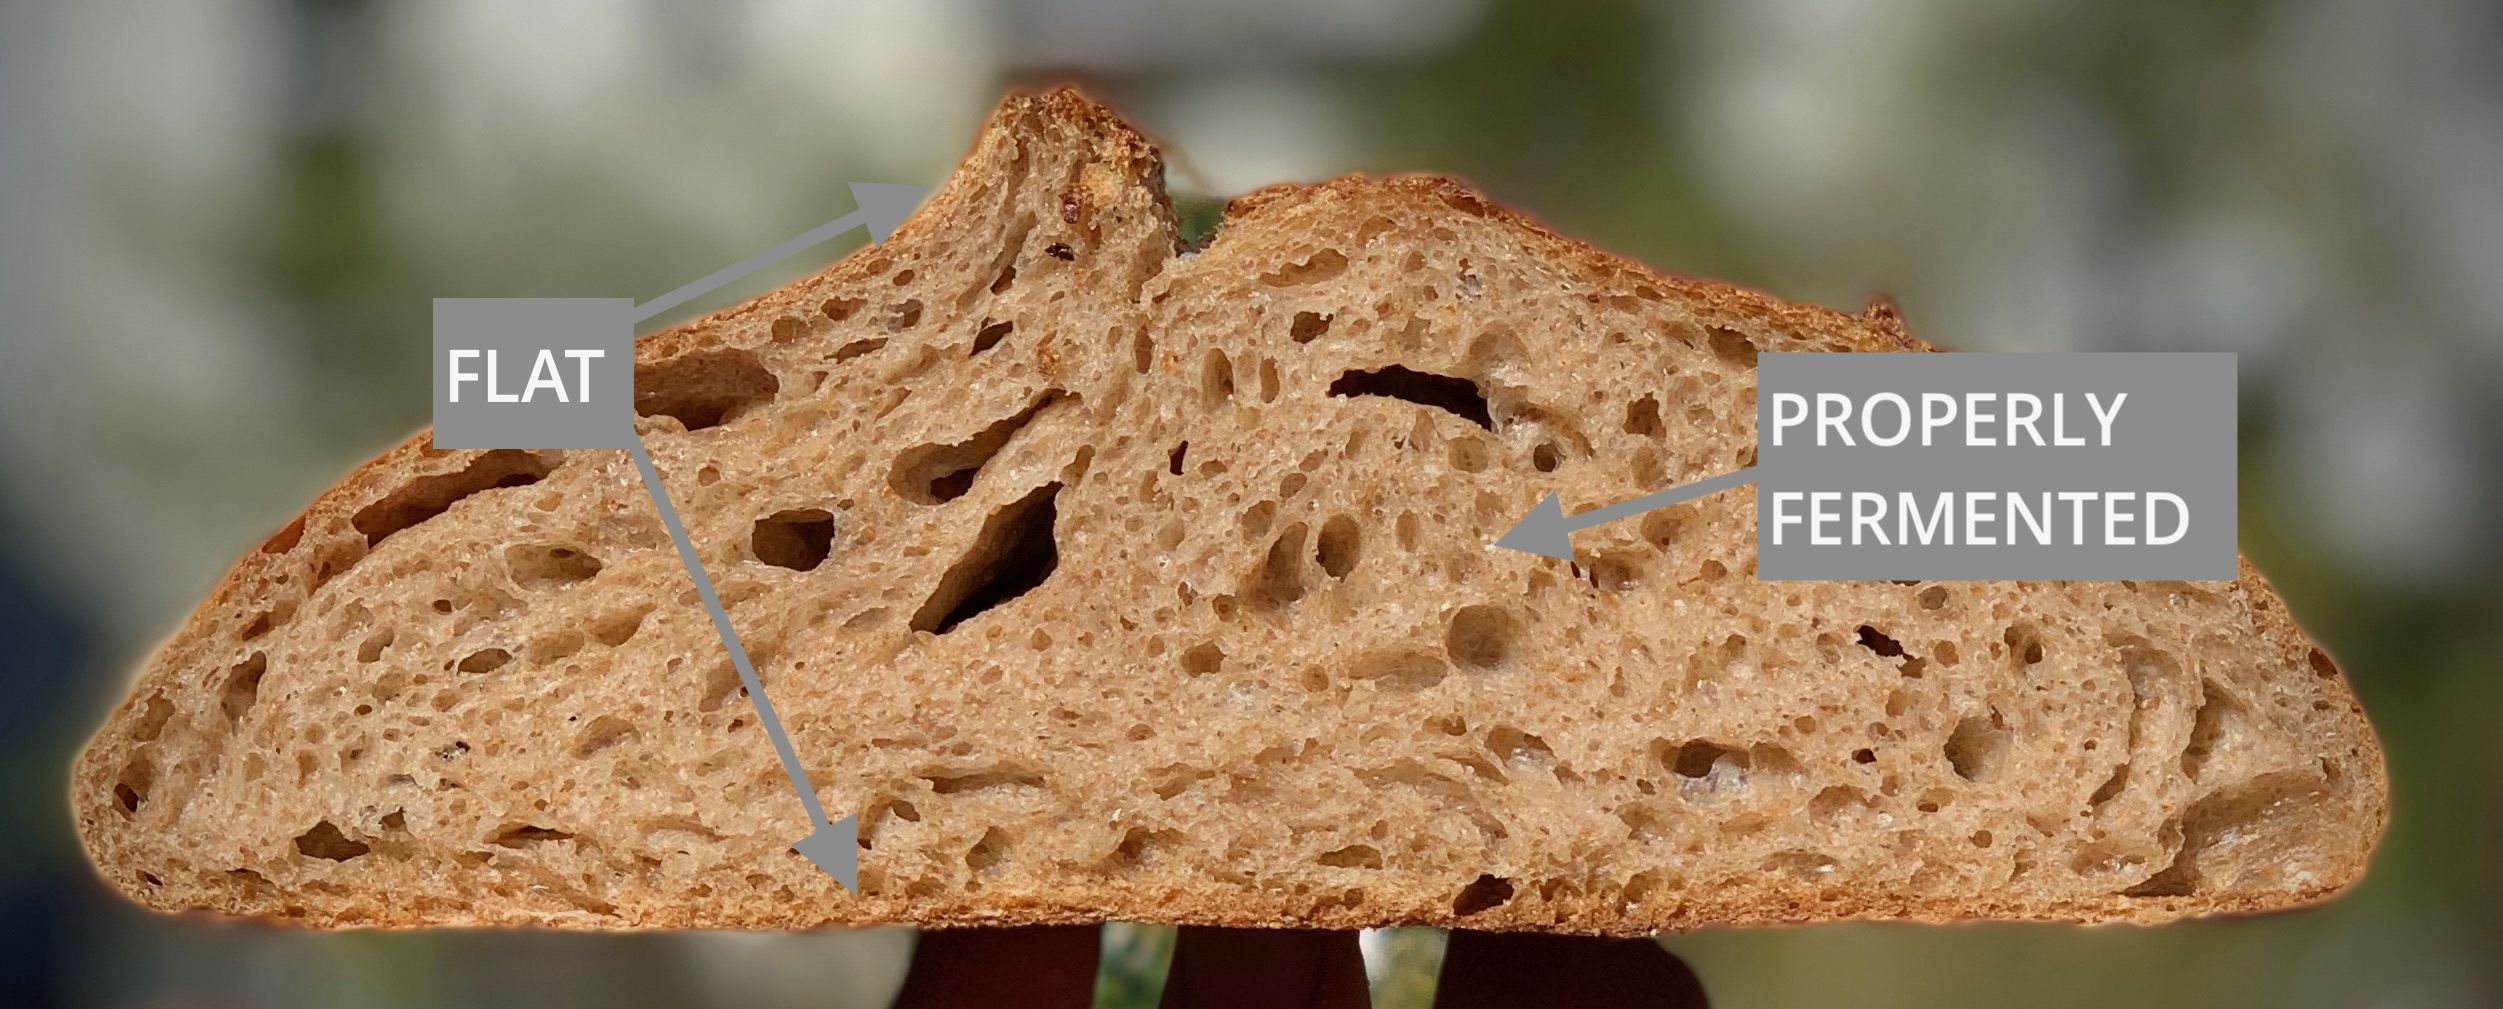
\includegraphics[width=\textwidth]{flat-bread}
  \caption{A very flat bread without enough dough strength.}%
  \label{flat-bread}
\end{figure}

When a dough flattens out quite a lot during the baking process, the chances are
that you did not create enough dough strength. This means your gluten matrix
hasn't been developed properly. Your dough is too extensible and flattens out
mostly rather than springing upwards in the oven. This can also happen if you
proofed your dough for too long. Over time the gluten relaxes and your dough
becomes more and more extensible. You can observe the gluten relaxing behavior
too when making a pizza pie. Directly after shaping your dough balls, it's very hard to shape
the pizza pie. If you wait for 30--90 minutes stretching the dough becomes a lot easier.

The easiest way to fix this is probably to knead your dough more at the start. To simplify
things consider using less water for your flour too. This will result in a more elastic dough
right away. This concept is commonly used for no-knead style sourdough.  Alternatively, you
can also perform more stretch and folds during the bulk fermentation process. Each
stretch and fold will help to strengthen the gluten matrix and make a more elastic dough.
The last option to fix a dough with too little dough strength is to shape your dough tighter.

\subsection{Baked too hot}

\begin{figure}
  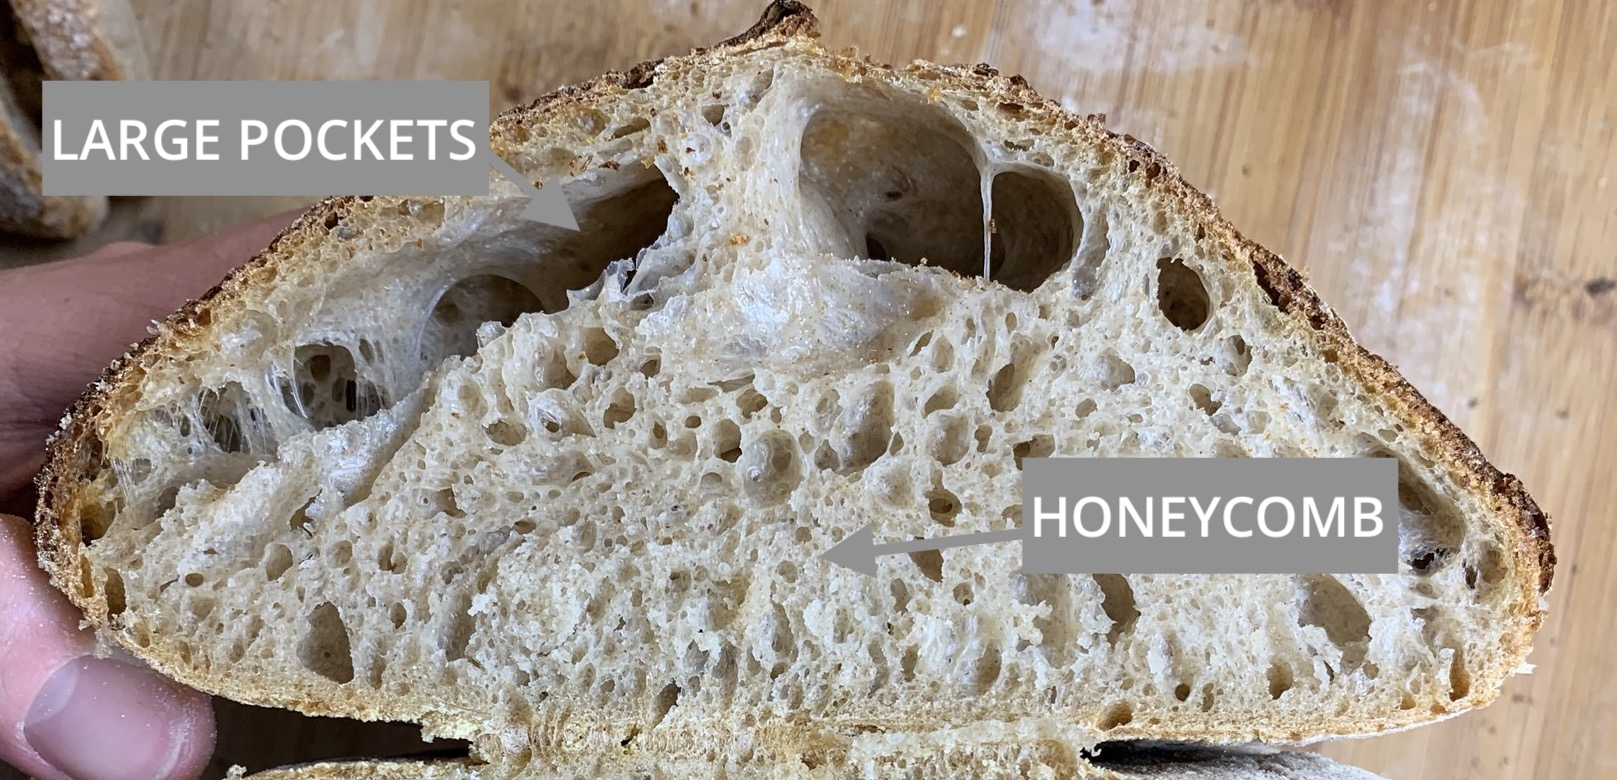
\includegraphics[width=\textwidth]{baked-too-hot-v2}
  \caption{A bread with very large alveoli close to the crust.}%
  \label{baked-too-hot}
\end{figure}

This is a common mistake that has happened to me a lot. When you bake your dough
at too high a temperature, you constrain your dough's expansion. The starch gelatinizes
and becomes more and more solid. At around 140°C (284°F) the Maillard reaction
starts to completely thicken your bread dough's crust. This is similar to baking
your bread dough without steam. As the internal dough's temperature heats up,
more and more water evaporates, gas expands and the dough is being pushed upwards.
Once the dough reaches the crust, it can no longer expand. The alveoli merge
into larger structures close to the surface of the dough. By baking too hot,
you are not achieving the ear which adds extra flavor. Furthermore, by restricting
it's expansion, the crumb will not be as fluffy as it could be.

If you have an extensible dough with high hydration, baking too cold will result
in the dough flattening out quite a lot. The gelatinization of the starch is
essential for the dough to hold its structure. After conducting several
experiments, it seems that my sweet spot for maximum oven spring seems to be
at around 230°C (446°F). Test the temperature of your oven, because in several
cases the displayed temperature might not match the actual temperature of your
oven~\cite{too+hot+baking}. Make sure to turn off the fan of your oven. Most
home ovens are designed to vent the steam as fast as possible. If you can not
turn the fan off, consider using a Dutch oven.

\subsection{Baked with too little steam}

\begin{figure}[h]
  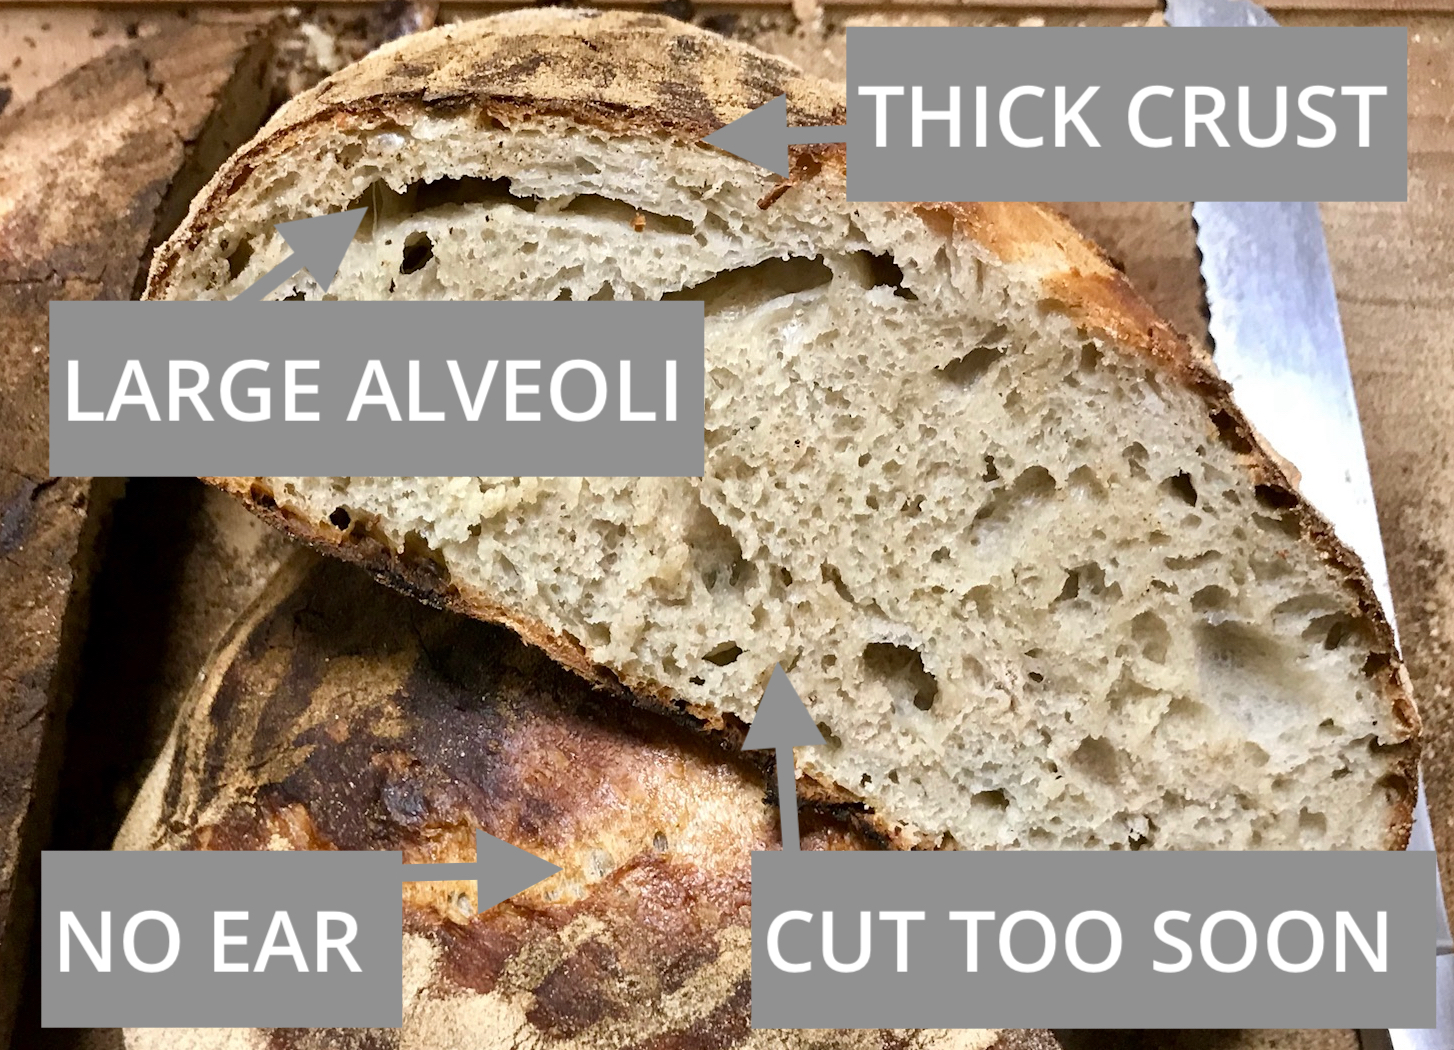
\includegraphics[width=\textwidth]{no-steam}
  \caption{One of my earlier breads that I~baked at a friend's place where
  I~couldn't steam the dough properly.}%
  \label{no-steam}
\end{figure}

Similar to baking too hot, when baking without enough steam, your dough's crust
forms too quickly. It's hard to spot the difference between the two mistakes.
I~typically first ask about the temperature and then about the steaming technique
to determine what might be wrong with the baking process. Too little steam can
typically be spotted by having a thick crust around all around your dough paired
with large alveoli towards the edges.

The steam essentially prevents the Maillard reaction from happening too quickly
on your crust. That's why steaming during the first stages of the bake is so important.
The steam keeps the temperature of your crust close to around 100°C (212°F). Achieving steam
can be done by using a Dutch oven, an inverted tray and/or a bowl of boiling water.
You might also have an oven with a built-in steam functionality. All the methods work,
it depends on what you have at hand. My default go-to method is an inverted
tray on top of my dough, paired with a bowl full of boiling water towards the bottom
of the oven.

\begin{figure}
  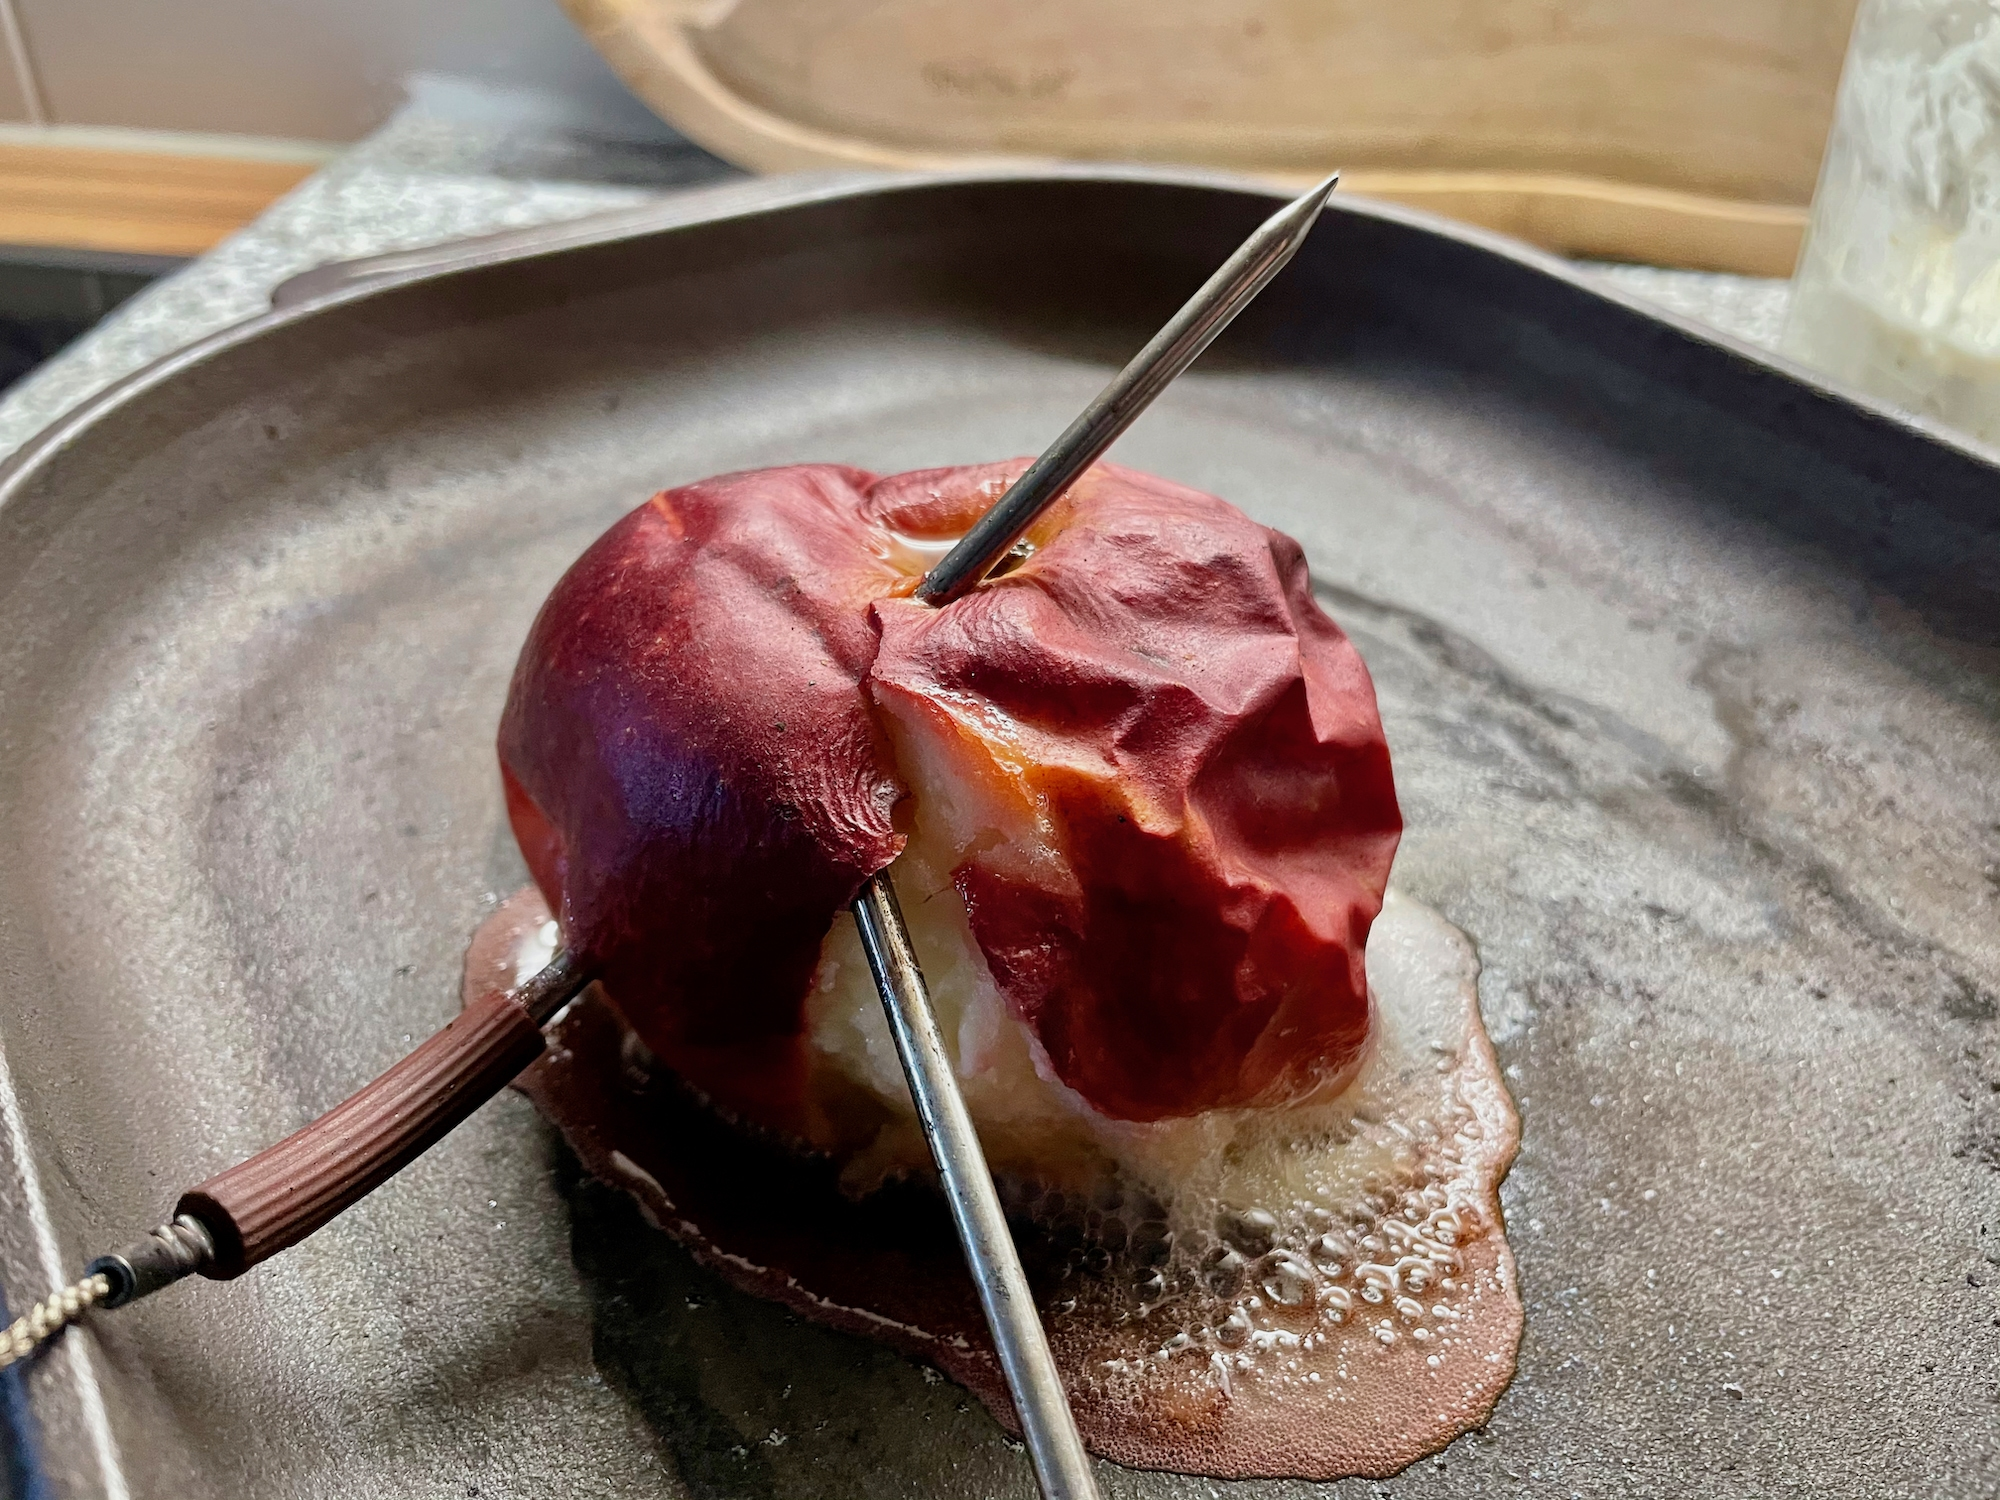
\includegraphics[width=\textwidth]{apple-experiment-temperatures}
  \caption{An apple with 2 probes to measure ambient
  and surface temperatures of several steaming techniques
  in a Dutch oven.}%
  \label{apple-experiment-temperatures}
\end{figure}

Now there can also be too much steam. For this I~tested using a Dutch oven paired with large ice
cubes to provide additional steam. The temperature of my dough's surface would directly
jump close to 100°C. The steam contains more energy and thus through convection
can heat up the surface of your dough faster. I~tested this by putting an apple inside
a Dutch oven and measuring its surface temperature using a barbecue thermometer.
I~then changed the steaming methods to plot how quickly the temperature
close to the surface changes. I~tested an ice cube inside of a preheated
Dutch oven, a preheated Dutch oven, a preheated Dutch oven with spritzes
of water on the apple's surface, a non-preheated Dutch oven where I~would only preheat
the bottom part. The experiment then showed that the ice-cube method would heat up
the surface of the apple a lot quicker. When replicating this with a bread dough,
I~would achieve less oven spring.

\begin{figure}[h]
  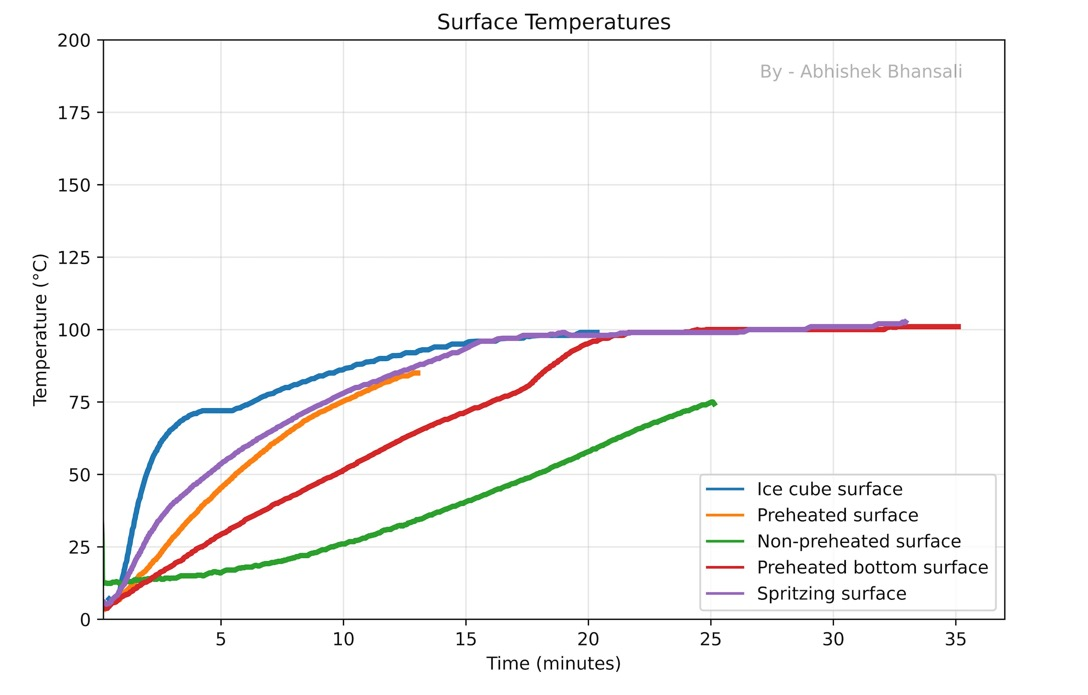
\includegraphics[width=\textwidth]{apple-experiment-surface-temperatures}
  \caption{A chart showing how the temperature of the surface
  of the apple changes with different steaming techniques.}%
  \label{apple-experiment-surface-temperatures}
\end{figure}

\begin{figure}[h]
  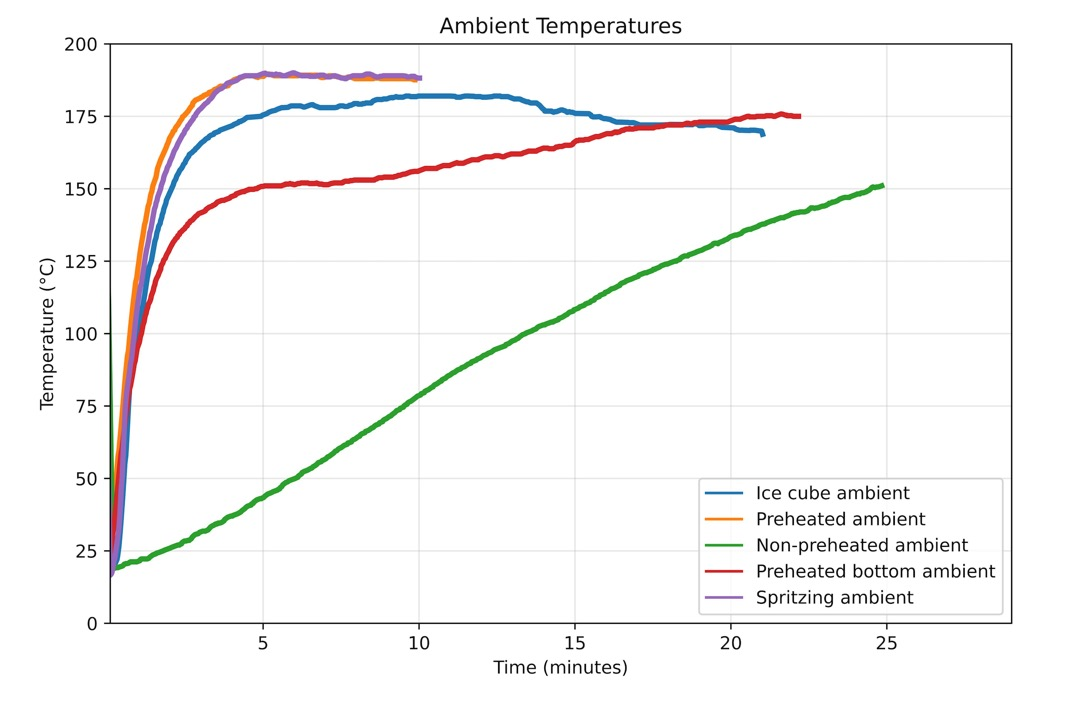
\includegraphics[width=\textwidth]{apple-experiment-ambient-temperatures}
  \caption{This figure shows how the ambient temperatures inside of the
  Dutch oven change depending on the steaming technique that is used.}%
  \label{apple-experiment-ambient-temperatures}
\end{figure}

Generally though, achieving too much steam is relatively challenging. I~could only
make this mistake when using a Dutch oven as the steaming method paired with relatively
large ice cubes. After talking with other bakers using the same Dutch oven, it seems
that my ice cubes (around 80g) were 4 times as heavy as the ones other bakers
would use (20g).

\section{Baking in the tropics}

Depending on the temperature, your fermentation speed adapts.
In a warmer environment, everything is faster. In a colder
environment, everything is slower.

This includes the speed at which your sourdough ferments
the dough but also the speed of enzymatic reactions. The
amylase and protease enzymes work faster, making more
sugars available and degrading the gluten proteins.

At around 22°C (72°F) in my kitchen my bulk fermentation is ready
after around 10 hours. I am using around 20 percent of sourdough
starter based on the flour. In summertime the temperatures
in my kitchen sometimes increase to 25°C (77°F). In that case
I am reducing the sourdough starter to around 10 percent.
If I didn't do that, my fermentation would be done after
around 4-7 hours. The problem is that the dough is quite
unstable when fermenting at this high speed. This means
that you are easily running into issues of over-fermentation.
Finding the perfect sweet spot between fermenting enough
and not too much is becoming much harder. Normally you might
have a time window of 1 hour. But at the rapid speed it
might be reduced to a time window of 20 minutes. Now at
30°C (86°F), ambient temperature things are much faster. Your bulk
fermentation might be complete in 2-4 hours when using
10-20 percent starter. Proofing your dough in the fridge
becomes almost impossible. As your dough cools down in the
fridge the fermentation also slows down. However cooling the
dough down from 30°C to 4-6°C in your fridge takes much
longer. Your dough is much more active compared to a dough
that starts at a temperature of 20-25°C. You might
end up overproofing your dough if you leave it overnight
in the fridge.

That's why I recommend that you reduce the amount of starter
that you use in the tropics to something at around 1-5 percent
based on the flour. This will slow down the fermentation
process significantly and provides you a bigger window
of time. Try to aim for an overall bulk fermentation of at
least 8-10 hours. Reduce the amount of starter to get there.

When making dough, try to use the same water temperature
as your ambient temperature. Assuming that the temperature
will climb to 30°C, try to start your dough directly
with 30°C water. This means that you can carefully rely on
a small fermentation sample that visualizes your fermentation
progress. The sample only works reliably if your dough temperature
is equal to your ambient temperature. Else the sample heats
up or cools down faster. So tread carefully when using
the sample in this case. It's always better to stop
the fermentation a little too early rather than too late.
Stretch and folds during the bulk fermentation
will help you to develop a better look and feel for
the dough. An expensive but possibly useful tool
could be a pH meter that allows you to perfectly
measure how much acidity has been created by the
lactic and acetic acid bacteria. In this case measure
the pH repeatedly and figure out a value that works
for your sourdough. In my case I tend to end bulk
fermentation at a pH of around 4.1. Please don't just
follow my pH value; it's very individual. Keep measuring
with different doughs to find out a value that works for you.

\section{My bread stays flat}

A flat bread is in most cases related to your gluten
network breaking down fully. This is not bad; this
means you are eating a fully fermented food. However,
from a taste and consistency perspective, it might be
that your bread tastes too sour, or is not fluffy anymore.
Please also note that you can only make bread with
great oven spring when making wheat based doughs. When
starting with this hobby I always wondered why my rye
breads would turn out so flat. Yes, rye has gluten, but
small particles called {\it hemicelluloses} (arabinoxylan and beta-glucan) \cite{rye-defects}.
prevent the dough from developing a gluten network like you can
do with wheat. Your efforts are in vain, and your dough will
stay flat. Only spelt- and wheat-based doughs have the capability
to retain the \ch{CO2} created by the fermentation.

In most cases something is probably off with your
sourdough starter. This very often happens when the starter
is still relatively young and hasn't yet matured
at fermenting flour. Over time your sourdough
starter is going to become better and better at fermenting
flour. Keep your sourdough starter at room temperature
and then apply daily feedings with a 1:5:5 ratio.
This would be 1 part old starter, 5 parts flour,
5 parts water. This allows you to achieve a better
balance of yeast and bacteria in your sourdough.
Even better could be the use of a stiff sourdough
starter. The stiff sourdough starter boosts
the yeast part of your starter. This allows you
to have less bacterial fermentation, resulting
in a stronger gluten network toward the end
of the fermentation \cite{stiff+starter}. Please
also refer to the section ~\ref{sec:overfermented-dough} where
I explained more about overfermented doughs. You can also
refer to section ~\ref{section:stiff-starter} with more details on
making a stiff sourdough starter.

Furthermore, a stronger flour containing more gluten
will help you to push the fermentation further. This
is because your flour contains more gluten and will
take longer to be broken down by your bacteria. Ultimately,
if fermented for too long, your dough is also going
to be broken down and will become sticky and flat.

To debug whether the excess bacterial fermentation is the issue,
simply taste your dough. Does it taste very sour? If yes,
that's a good indicator. When working the dough, does it
suddenly become very sticky after a few hours? That's a
another good indicator. Please also use your nose to note
the smell of the dough. It shouldn't be too pungent.

\section{I want more tang in my bread}

To achieve more tang in your sourdough bread, you have
to ferment your dough for a longer period of time.
Over time the bacteria will metabolize most of the
ethanol created by the yeast in your dough. The bacteria
mostly produce lactic and acetic acid. Lactic acid
is chemically more acidic than acetic acid but sometimes
not perceived as sour. In most cases a longer fermentation
is what you want. You will either need to utilize a loaf
pan to make your dough or use a flour that can withstand
a long fermentation period. A flour like this is typically
called a {\it strong flour}. Stronger flours tend
to be from wheat varieties that have be grown in more
sunny conditions. Because of that, stronger flours tend
to be more expensive. For freestanding loaves, I recommend
using a flour that contains at least 12 percent protein.
Generally, the more protein, the longer you can ferment your dough.

Another option to achieve a more sour flavor could be to
use a starter that produces more acetic acid. Based on my own
experience, most of my pure rye starters produced stronger acetic
notes. Chemically, the acetic acid isn't as sour, but when tasting
it will seem more sour. Make sure to use a starter that is at
a hydration of around 100 percent. Acetic acid production
requires oxygen. A too-liquid starter tends to favor lactic
acid production because the flour is submerged in water, no
oxygen can reach the fermentation after a while.

\begin{figure}[!htb]
  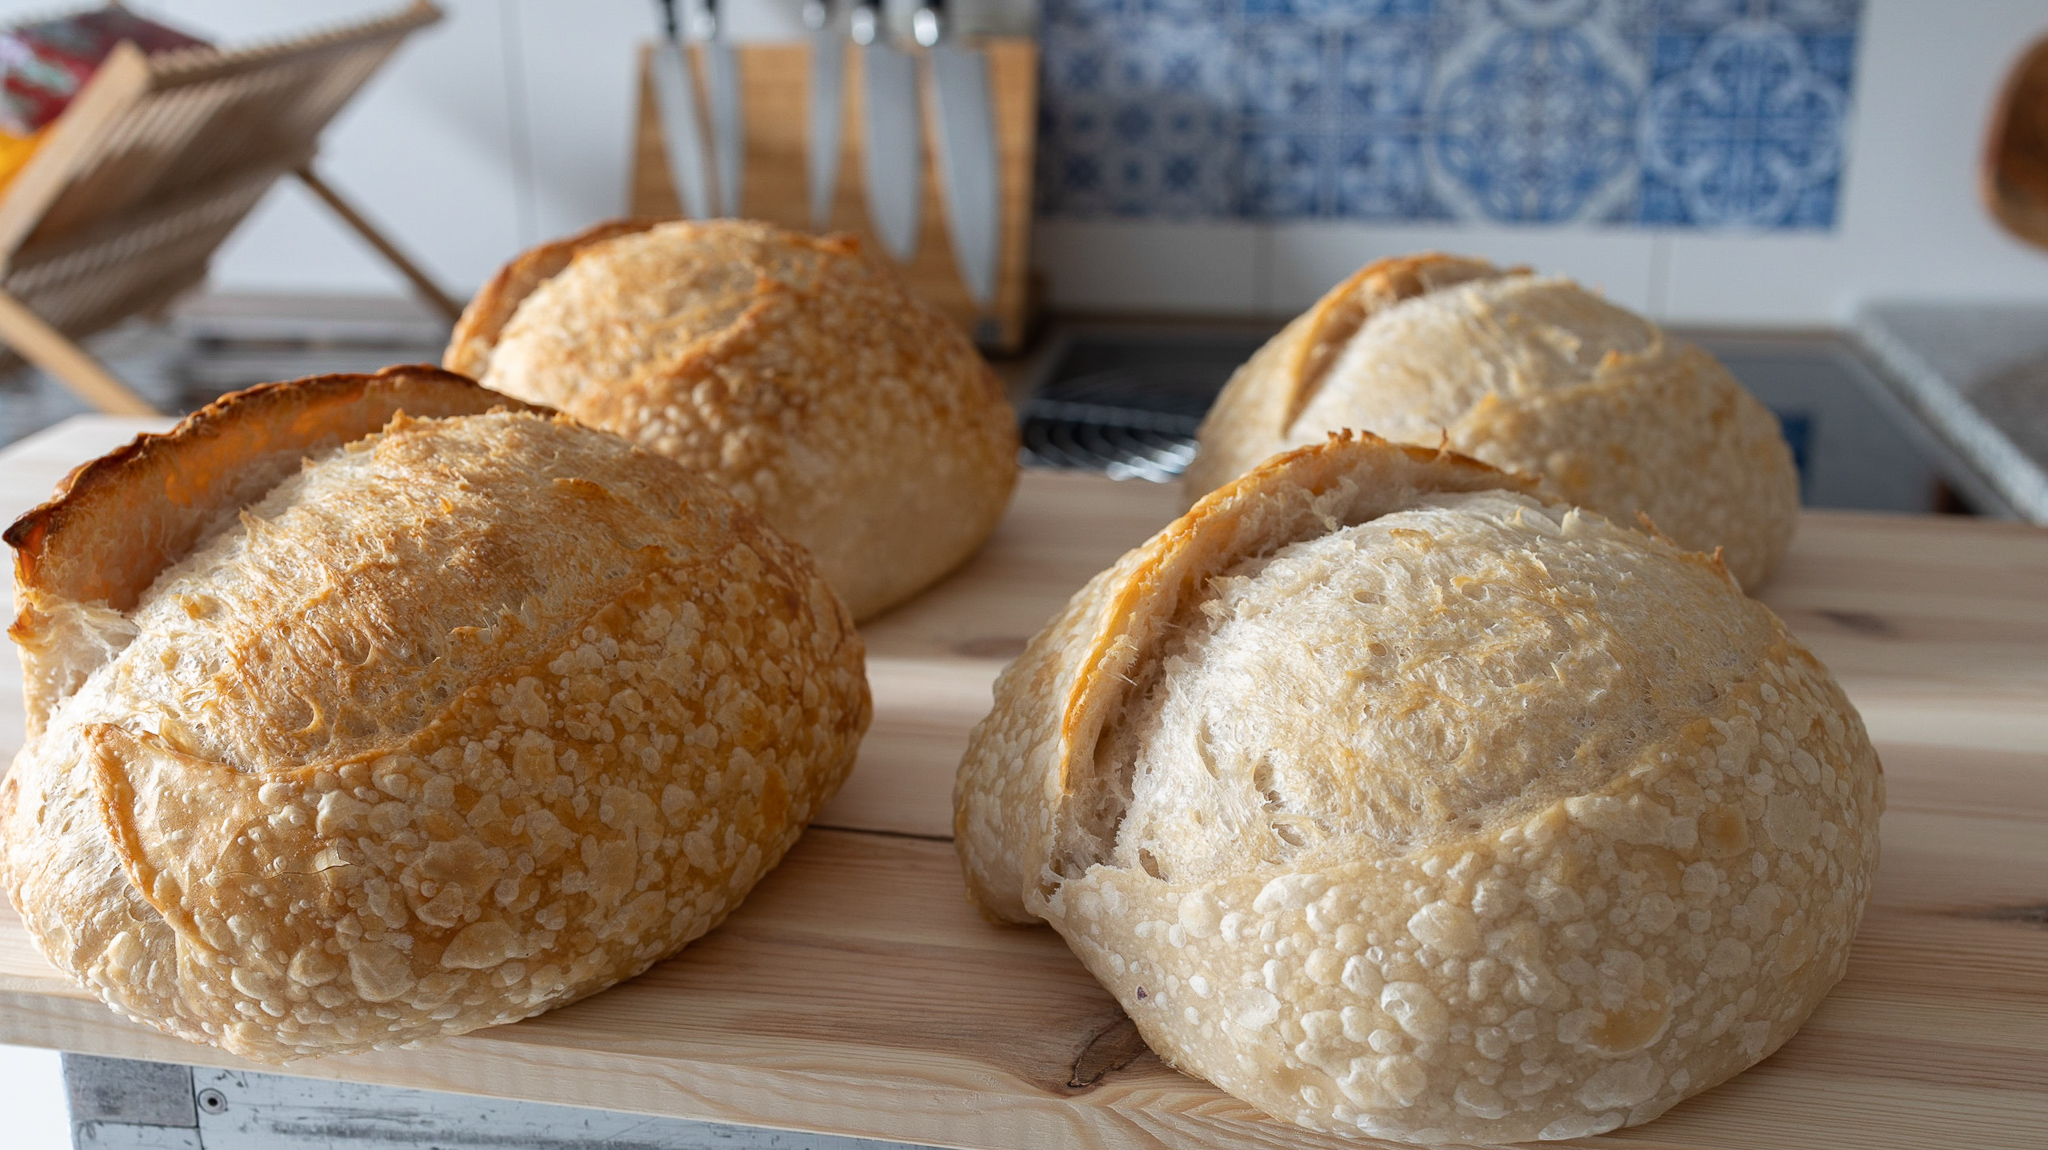
\includegraphics[width=\textwidth]{parbaked-bread.jpg}
  \caption{A half-baked bread, known as "parbaked".}
  \label{fig:parbaked-bread}
\end{figure}

Another easier option could be to bake your sourdough
twice. I have observed this when shipping bread for my micro
bakery. The idea was to bake my bread for around 30 minutes
until it's sterilized, let it cool down and then ship it
to customers. Once you receive it, you just bake it again
for another 20-30 minutes to achieve the desired crust and
then you can eat it. Some of the customers reported a very sour
tasting bread. After investigating a bit more, it became
crystal clear. By baking the bread twice you don't boil
as much of the acid during the baking process. Water
evaporates at around 100°C (212°F) while acetic acid boils at
118°C (244°F) and lactic acid at 122°C (252°F). After baking for 30 minutes
at around 230°C (446°F) some of the water has started to evaporate,
but not all the acid yet. If you were to continue to bake, more
and more of the acid would start to evaporate. Now if you were
to stop baking after 30 minutes, you would typically have reached
a core temperature of around 95°C (203°F). Your dough would need
to be cooled down again to room temperature. The crust would
still be quite pale. Then a couple of hours later, you start
to bake your dough again. Your crust would become nice and
dark featuring delicious aroma. The aroma is coming from the
Maillard reaction. However, the core of your dough still won't
exceed the 118°C required to boil the acid. Overall, your
bread will be more sour. The enhanced acidity also helps
to prevent pathogens from entering your bread. The bread
will be good for a longer period of time. That's why
the concept of a delivery works well with sour sourdough bread.
In my experiments the bread stayed good for up to a week
in a plastic bag.

\section{My bread is too sour}

Some people like the bread less sour as well. This
is personal preference. To achieve a less sour bread
you need to ferment for a shorter period of time.
The yeast produces \ch{CO2} and ethanol. Both yeast and
bacteria consume the sugars released by the amylase enzyme
in your dough. When the sugar is depleted, bacteria starts to
consume the leftover ethanol by the yeast. Over time more
and more acidity is created, making a more sour loaf.

Another angle at this would be to change the yeast/bacteria
ratio of your sourdough. You can start the fermentation with
more yeast and less bacteria. This way, for the same given
volume increase of your dough, you will have less acidity.
A really good trick is to make sure that you feed your starter
once per day at room temperature. This way you shift
the tides of your starter towards a better yeast fermentation \cite*{more+active+starter}.

To shift the tides even further, a real game changer
to me has been to create a stiff sourdough starter. The
stiff sourdough starter is at a hydration of around 50 percent.
By doing so your sourdough starter will favor yeast
activity a lot more. Your doughs will be more fluffy and will
not as sour for a given volume increase. I tested this
by putting condoms over different glass jars. I used
the same amount of flour for each of the samples.
I tested a regular starter, a liquid starter and a stiff
starter. The stiff starter by far created the most \ch{CO2}
compared to the other starters. The balloons were inflated
the most. \cite{stiff+starter}

Another unconventional approach could be to add baking
powder to your dough. The baking powder neutralizes the
lactic acid and will make a much milder dough.\cite{baking+powder+reduce-acidity}

\section{Fixing a moldy sourdough starter}

First of all, making a moldy sourdough starter is very difficult.
It's an indicator that something might be completely off in your starter.
Normally the symbiosis of yeast and bacteria does not allow external
pathogens such as mold to enter your sourdough starter.
The low pH created by the bacteria is a very hostile environment
that no other pathogens like. Generally everything below a pH
of 4.2 can be considered food safe\cite{food+safe+ph}. This
is the concept of pickled foods. And your sourdough bread
is essentially pickled bread.

I have seen this happening especially when the sourdough
starter is relatively young. Each flour naturally contains
mold spores. When beginning a sourdough starter, all
the microorganisms start to compete by metabolizing the
flour. Mold can sometimes win the race and outcompete
the natural wild yeast and bacteria. In that case simply
try cultivating your sourdough starter again. If it molds
again, it might be a very moldy batch of flour. Try a different
flour to begin your sourdough starter with.

Mature sourdough starters should not mold unless the conditions
of the starter change. I have seen mold appearing when the starter is stored
in the fridge and the surface dried out. It also sometimes forms on the
edges of your starter's container, typically in areas where no active
starter microorganisms can reach. Simply try to extract an
area of your starter that has no mold. Feed it again with flour and
water. After a few feedings, your starter should be back to normal.
Take only a tiny bit of starter: 1-2 grams are enough. They already
contain millions of microorganisms.

Mold favors aerobic conditions. This means that air is required in order
for the mold fungus to grow. Another technique that has worked for me
was to convert my sourdough starter into a liquid starter. This successfully
shifted my starter from acetic acid production to lactic acid production.
Acetic acid, similarly to mold, requires oxygen to be produced. After
submerging the flour with water, over time the lactic acid bacteria
outcompeted the acetic acid bacteria. This is a similar concept to pickled
foods. By doing this you are essentially killing all live mold fungi. You
might only have some spores left. With each feeding the spores will become
fewer and fewer. Furthermore, it seems that lactic acid bacteria produce
metabolites that inhibit mold growth. \cite{mold+lactic+acid+bacteria}

\begin{figure}[!htb]
  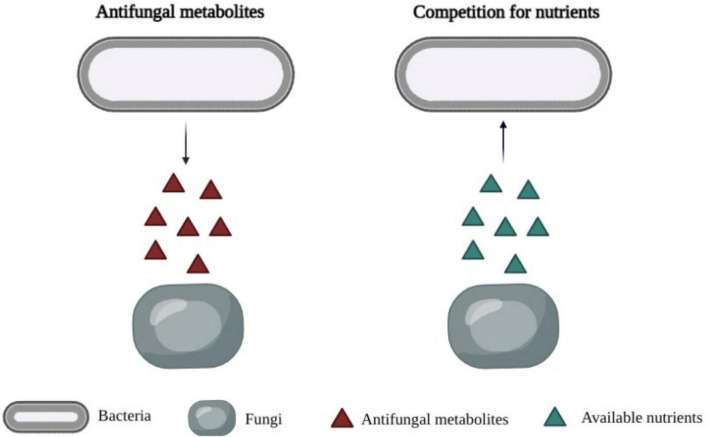
\includegraphics[width=\textwidth]{fungi-lactic-acid-interactions}
  \caption{The interaction of lactic acid bacteria and mold fungi.
           The authors Ce Shi et al. show how bacteria are producing
           metabolites that inhibit fungus growth. \cite{mold+lactic+acid+bacteria}}
  \label{fig:fungi-lactic-acid-interactions}
\end{figure}

To pickle your starter, simply take a bit of your existing starter (5 grams for
instance). Then feed the mixture with 20g of flour and 100g of water. You have
created a starter a hydration of around 500 percent. Shake the mixture vigorously.
After a few hours you should start seeing most of the flour near the bottom
of your container. After a while most of the oxygen from the bottom mixture
is depleted and anaerobic lactic acid bacteria will start to thrive. Take a
note of the smell your sourdough starter. If it was previously acetic
it will now change to be a lot more dairy. Extract a bit of your mixture the
next day by shaking everything first. Take 5g of the previous mixture, feed
again with another 20g of flour and another 100g of water. After 2-3
additional feedings your starter should have adapted. When switching back
to a hydration of 100 percent the mold should have been eliminated. Please note that
more tests should be conducted on this topic. It would be nice to really
carefully analyze the microorganisms before the pickling and after.

\section{My bread flattens out when removing it from the banneton}

After removing your dough from the banneton, your dough will always
flatten out a bit. That's because over time your gluten network
relaxes and can no longer hold the shape. However, during the course
of baking, your dough is going to increase in size and inflate again.

If your dough however flattens out completely, it's a sign that
you have fermented your dough for too long. Please refer to ~\ref{sec:overfermented-dough}
where I explain about overfermented doughs. Your bacteria
has consumed most of your gluten network. That's why your
dough fully collapses and stays flat during the bake. The
\ch{CO2} and evaporating water will diffuse out of the dough.
A related symptom is that your dough sticks to the banneton.
When I starting baking I combated this with rice flour.
It worked for me but it might be a false find. These days I gently rub my
dough with a bit of non-rice flour before placing it in
the banneton. Now if the dough starts to stick to the banneton
while I remove it I resort to a drastic measure. I immediately
grease a loaf pan and directly place the dough inside. The loaf
pan provides a barrier and the dough can't flatten out as much.
The dough won't be as fluffy but it will be super delicious if you love tangy bread.

If you own a pH meter, take a note of your dough's pH before baking.
This will allow you to better judge your dough throughout
the fermentation process.

\section{My bread flattens out during shaping}

Similarly to a dough flattening out after removing it from the banneton,
a flattened dough after shaping is also a possible sign of over-fermentation.

When you try to shape the dough, can you easily tear pieces from the dough?
If yes, you have definitely overfermented your dough. If not, it might just
be a sign that you have not created enough dough strength for your dough.
A ciabatta, for instance, is a dough that tends to flatten out a bit after shaping.

If your dough is not able to be shaped at all, use a greased loaf pan
to rescue your dough. You can also cut a piece of the dough and use it
as the starter for your next dough. Your sourdough dough is essentially
just a gigantic starter.

\section{Liquid on top of my starter}

Sometimes a liquid, in many cases black liquid, gathers on top
of your sourdough starter. The liquid might have a pungent
smell to it. Many people confuse this with mold. I have seen
bakers recommending to discard the starter because of this liquid.
The liquid is commonly known as {\it hooch}. After a while
of no activity the heavier flour separates from the water. The flour
will sit at the bottom of your jar and the liquid will stay on top.
The liquid turns darker because some particles of the flour weigh
less than the water and float on top. Furthermore dead microorganisms
float in this liquid. This liquid is not a bad thing; it's actively
protecting your sourdough starter from aerobic mold entering through
the top.

\begin{figure}[!htb]
  \centering
  \includegraphics[width=0.5\textwidth]{hooch}
  \caption{Hooch building on top of a sourdough starter. \cite{liquid+on+starter}}
  \label{fig:hooch}
\end{figure}

Simply stir your sourdough starter to homogenize the hooch back
into your starter. The hooch will disappear. Then use a little bit of
your sourdough starter to set up the starter for your next bread.
Once hooch appears, your starter has likely fermented for a long
period of time. It might be very sour. This state of starter
is excellent to make discard crackers or a discard bread. Don't throw
anything away. Your hooch is a sign that you have a long fermented
dough in front of you. Compare it to a 2 year ripened Parmigiano cheese.
The dough in front of you is full of delicious flavor.

\section{Why does my starter smell like vinegar or acetone?}

Your sourdough starter has likely produced a lot of acetic acid.
Acetic acid is essential when creating vinegar. Once no additional
food is left some of your starter's bacteria will consume ethanol
and convert it into acetic acid. Acetic acid has a very pungent smell.
When tasting acetic acid, the flavor of your bread is often perceived
as quite strong.

\begin{figure}[!htb]
  \centering
  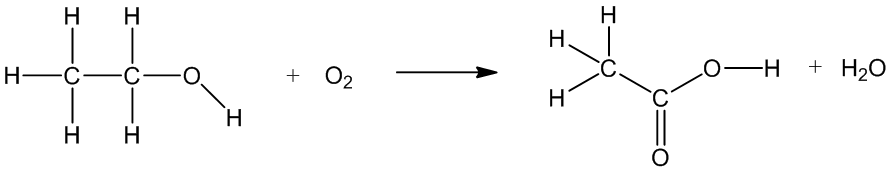
\includegraphics[width=1.0\textwidth]{ethanol-oxidation}
  \caption{Oxygen is required to create acetic acid \cite{acetic+acid+production}.}
  \label{fig:ethanol-oxidation}
\end{figure}

This is nothing bad. But if you would like to change
the flavor of your final bread, consider converting
your sourdough starter into a liquid starter. This will
help to prioritize lactic acid-producing bacteria.
Your flavor will change to dairy compared to vinegary.
You can't go back though. After the conversion your starter
will never go back to acetic acid production because you have
changed the tides towards primarily lactic acid fermentation.
I like to have a separate rye starter. In my experiments
rye starters tend to feature many acetic acid bacteria.
This starter is excellent when you want to make a very hearty,
strong-tasting bread. A pure rye bread tastes excellent when
made with such a starter. The flavor when taking a bite
is incredible. It nicely plays with soups as well. Just take
a bit of this bread and dip it in your soup.

\section{My crust becomes chewy}

Depending on which style of bread you are making a
thick crackly crust is sometimes desired. The crust
of your bread is created during the 2nd stage of the
baking process once the steaming source of your
oven has been removed. The dark colors are created by
the process known as {\it Maillard reaction} and then followed
by another process known as {\it caramelization}. Each
color of crust offers the taster a different aroma.

What happens quite often is that the crust becomes chewy after a day.
Sometimes when baking in the tropics with high humidity, the
crust only stays in this stage for a few hours. Afterwards
the crust becomes chewy. It's no longer as crisp compared
to the moment after baking. Your dough still contains moisture.
This moisture will start to homogenize in the final bread and
partially evaporate. The result is that your crust becomes chewy.

Similarly when storing your bread in a container or in a plastic
bag, your crust is going to become chewy. I have no fix for this yet.
I typically tend to store my breads in a plastic bag inside of my fridge.
This allows the moisture to stay inside of bread. When taking a slice
I always toast each slice. This way some of the crispness returns.
If you know of a great way, please reach out and I will update
this book with your findings.

\section{My dough completely tears after a long fermentation}

Sometimes when touching your dough after a long fermentation
it completely tears apart. This could be for two reasons. It might
be that the bacteria completely consumed the gluten of your flour.
On the other hand, over time your gluten network automatically
degrades. This is the protease enzyme converting the gluten
network into smaller amino acids the seedling can use as
building blocks for its growth. This process starts to happen
the moment you mix flour and water. The longer your dough sits,
the more gluten is broken down. As the gluten holds the
wheat dough together, your dough will ultimately tear.

\begin{figure}[!htb]
  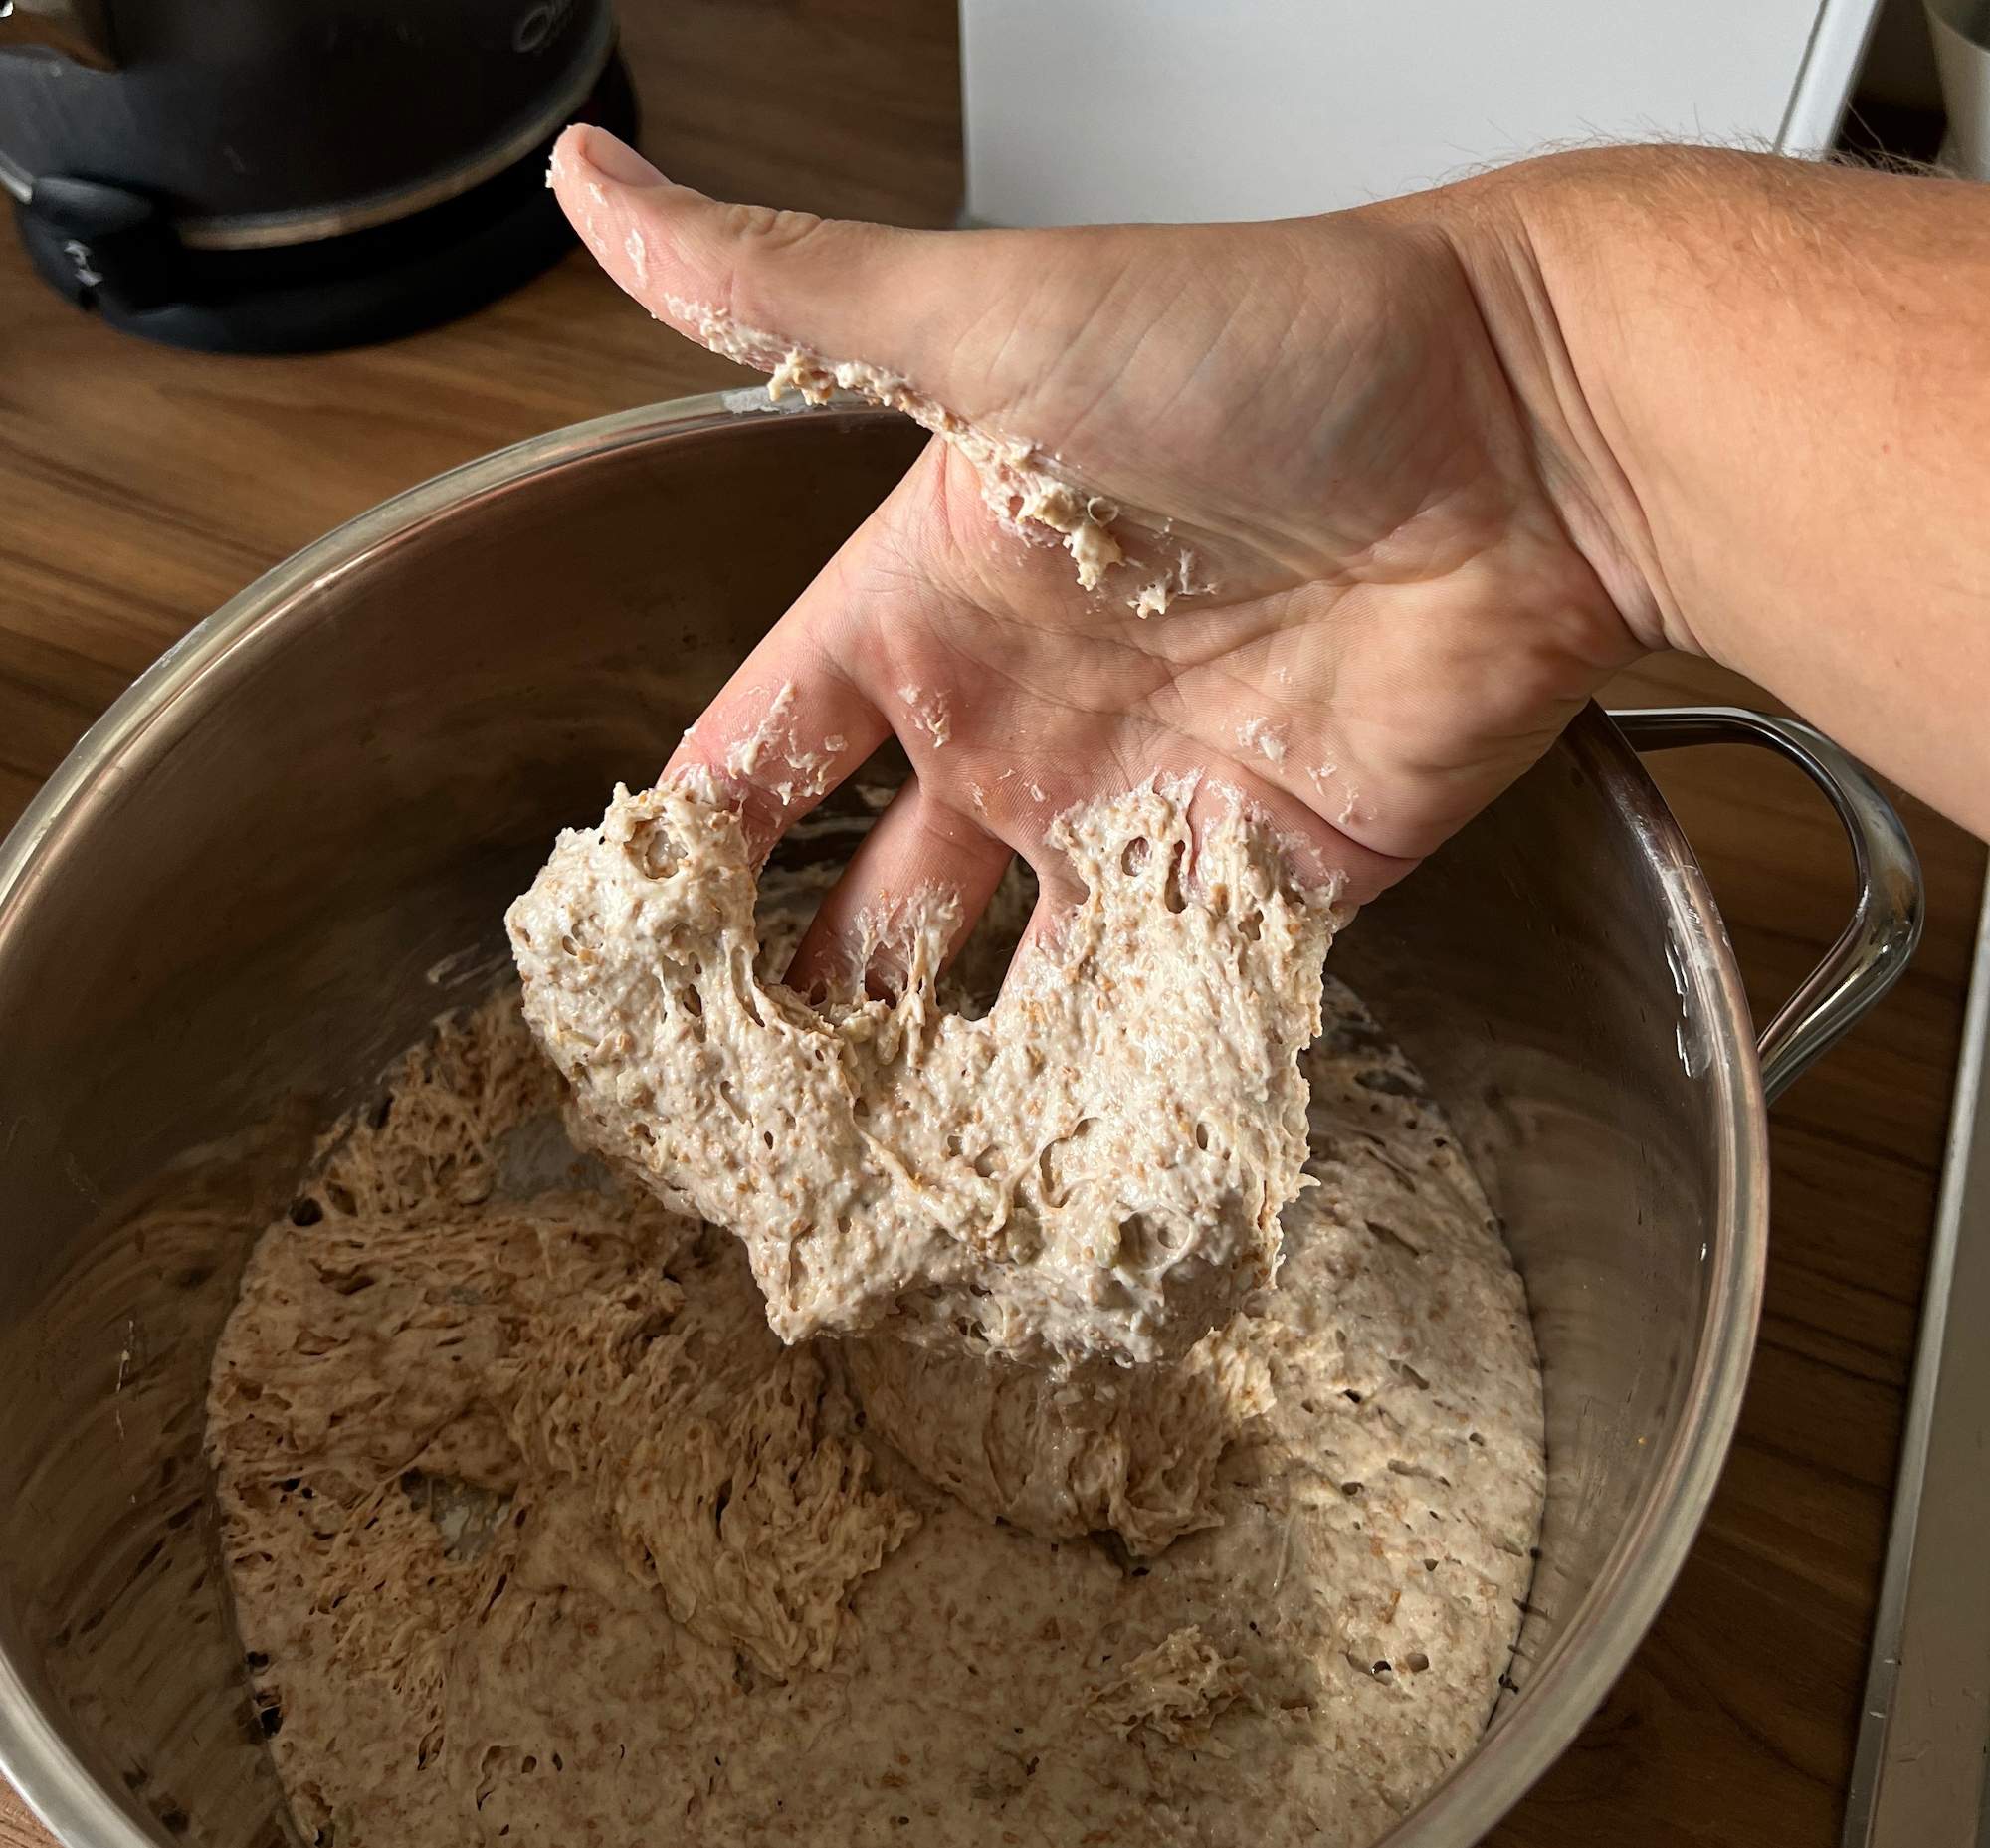
\includegraphics[width=1.0\textwidth]{tearing-dough}
  \caption{My dough tearing after 24 hours of no activity}
  \label{fig:tearing-dough}
\end{figure}

In the picture~\ref{fig:tearing-dough} I experimented with
using a starter that has not been fed for 30 days at room temperature.
I tried to make a dough directly out of the unfed starter.
Typically after a long period
without feedings your microbes start to sporulate and go
into hibernation mode. This way they can survive for a long
period of time without extra feedings. Adding additional food
will activate them again. In this case the dough did not ferment
fast enough before the protease broke down the gluten. By activating
your microbes they will start to reproduce and increase in quantity
for as long as there is food available. But this process
in my case was not fast enough. After around 24 hours, the whole
dough just started to completely tear apart. The whole process was further
accelerated by my using whole wheat flour. Whole wheat
contains more enzymes than white flour.

To fix this, try to make sure that your sourdough starter is lively
and active. Simply apply a couple of more feedings in advance before
making your dough. This way your dough becomes ready to shape
before it has completely broken down.

\section{My sourdough starter is too sour}

A too-sour sourdough starter will cause problems during
the fermentation. Your fermentation will be more on the
bacterial side, rather than the yeast side. This means
you will likely create a more tangy loaf which isn't
as fluffy as it could be. The goal is to reach the right
balance: Fluffy consistency from the yeast and a great,
not-too-strong tang from the bacteria. This depends
of course on what you are looking for in terms of taste
in your bread. When making rye bread, I prefer to be more
on the tangy side for instance. When the described balance
is off, the first thing to check is your sourdough starter.

Note the smell of your starter. Does it smell very sour?
Taste a bit of your starter too. How sour does it taste?
Over time, every starter becomes more and more sour the longer
you wait. But sometimes your starter becomes sour too fast.
In this case apply daily feedings to your starter. Reduce
the amount of old starter that you use to feed. A ratio
of 1:5:5 or 1:10:10 can do wonders. In this case you would
take 1 part of starter (10g) and feed it with 50g of flour
and 50g of water. This way the microorganisms start
the fermentation in a green field environment. This is
similar to the 10 percent starter of 20 percent starter
ratio that you use to make a dough. These days I almost
never use a 1:1:1 ratio. This only makes sense when you
are initially creating your starter. You want a sour
environment so that your microorganisms outcompete
potential pathogens. The acidic environment is toxic
to most pathogens that you do not want in your starter.

Another approach that can help is to convert your
sourdough starter into a stiff starter as
described in section \ref{section:stiff-starter}.

\section{My starter does not double in size}

Some bakers call for the sourdough starter to
double in size before using it.
The idea is to use the sourdough starter at
peak performance to ensure a
balanced fermentation in the main dough.

The doubling in size metric should be
taken with a grain of salt when judging
your starter. Depending on the flour
you use to feed the starter, different levels
of its rising can be expected.
For instance, if you use rye flour then only
very little gas from the
fermentation can be retained inside the
starter. In consequence, your
sourdough starter will not rise as much. It
could still be in healthy shape. If you use wheat flour with less gluten,
the starter will not rise as
much either. The reason is that you have a weaker
gluten network resulting in
more gas dispersing out of your dough.

That being said, it is recommended that you develop
your volume increase
metric. Your starter will increase in size and then
ultimately lose structure
and collapse. Observe the point before it collapses.
This is the point when
you should use your starter. This could be a
50 percent volume increase, 100
percent or 200 percent. It is always better to use
the starter a little bit
too early rather than too late. If you use the
starter later, reduce the
quantity that you use. If the recipe calls for a 20
percent starter quantity,
use only 10
percent starter in that case. Your starter will
regrow in your main dough.

On top of relying on the size increase, start
taking note of your starter's
smell. Over time you will be able to judge its
fermentation state based on the
smell. The stronger the smell becomes, the further
your dough has fermented.
This is a sign that you should use less starter
when making the actual dough.

Please refer to section \ref{section:readying-starter} "\nameref{section:readying-starter}"
for more information on the topic.

\section{Should I autolyse my dough?}

In 95 percent of all cases, an autolysis
makes no sense. Instead I recommend
that you conduct a fermentolysis. You
can read more about the autolysis process in
section \ref{section:autolysis} and
more about the topic of fermentolysis
in section \ref{section:fermentolysis}.

The fermentolysis combines all the benefits
of the autolysis while eliminating disadvantages
such as having to knead the dough multiple times.

The autolysis only makes sense when you might
bake a fast-fermenting yeast-based dough with a
high yeast inoculation rate. But even in that
case you could just lower the amount of yeast
to fermentolyse rather than autolyse.

\section{What's the benefit of using a stiff sourdough starter?}

A regular sourdough starter has equal parts of
flour and water (100 percent hydration). A stiffer
sourdough starter features a hydration level of 50 to 60 percent.

The stiff sourdough starter boosts the yeast part
of your starter more. This way your gluten degrades
slower and you can ferment for a longer period. This
is especially handy when baking with lower gluten flours.

You can read more about the topic of stiff sourdough
starters in section \ref{section:stiff-starter}.

\section{What's the benefit of using a liquid sourdough starter?}

The liquid starter will boost anaerobic bacterial
fermentation in your starter. This way your starter
tends to produce more lactic acid rather than acetic
acid. Lactic acid is perceived as milder and more
yogurty. Acetic acid can sometimes taste quite
pungent. Acetic acid can be perfect when making 
dark rye bread but not so much when making a fluffy
ciabatta-style loaf.

When converting your starter to a liquid starter you are
permanently altering the microbiome of your starter.
You cannot go back once you have eliminated acetic
acid-producing bacteria. So it is recommended to keep
a backup of your original starter.

A downside to the liquid starter is the overall
enhanced bacterial activity. This means the baked bread
will have more acidity (but milder). The dough will degrade
faster during fermentation. For this reason, you
will need to use strong high-gluten flour when using
this type of starter.

You can read more about the liquid starter
in section \ref{section:liquid-starter}

\section{My new starter doesn't rise at all}

Make sure that you use unchlorinated water.
In many areas of the world, tap water has
chlorine added to kill microorganisms. If that's
the case in your region, bottled spring water will
help.
You can also use a water filter with activated charcoal
which will remove the chlorine.
Alternatively, if you draw tap water into a pitcher or other
container and let it sit, loosely covered, the chlorine
should dissipate within 12-24 hours, and you have
the added advantage of automatically having
room-temperature water.

Make sure to use whole grain flour (whole wheat, whole rye, etc.).
These flours have more natural wild yeast and
bacterial contamination. Making a starter
from just white flour sometimes doesn't work.
Try to use organic unbleached flour to make
the starter. Industrial flour can sometimes
be treated with fungicides.

\section{I made a starter, it rose on day 3 and now not anymore}

This is normal. As your starter is maturing, different
microorganisms are activated. Especially during
the first days of the process, bad microbes
like mold can be activated. These cause your
starter to rise a lot. With each subsequent
starter-feeding, you select the microbes that are best
at fermenting flour. For this reason, it is
recommended to discard the leftover unused starter
from the first days of the process. Later on, unneeded
starter amounts should never be thrown away. You can make
great discard bread out of it.

So just keep going and don't give up. The first big
rise is an indicator that you are doing everything
right. Based on my experience, it takes around 7
days to grow a starter. As you feed your starter
more and more, it will become even better at fermenting
flour. The first bread might not go exactly as you
planned, but you will get there eventually. Each
feeding makes your starter stronger and stronger.

\section{My flour has low gluten content - what should I do?}

You can always mix in a little bit of vital wheat gluten. Vital wheat gluten
is concentrated extracted gluten from wheat flour.

I recommend that you add around 5 grams of wheat gluten for every 100 grams of
flour that you are using.

\section{What's a good level of water (hydration) to make a dough?}

Especially when starting to make bread, use lower amounts of water. This will
greatly simplify the whole process. I recommend using a level of around 60
percent hydration. So for every 100 grams of flour use around 60 grams of water.
This ballpark figure will work for most flours. With this hydration, you can
make bread, buns, pizzas, and even baguettes out of the same dough.

With the lower hydration, dough handling becomes easier and you have more yeast
fermentation, resulting in lower over-fermentation risk.

\section{What's the best stage to incorporate inclusions (seeds) into the dough?}

You can include seeds directly at the start when mixing the dough. If you use
whole seeds such as wheat or rye kernels, soak them in water overnight and
then rinse them before adding them to the dough. This makes sure that they
are not crunchy and are soft enough when eating the bread. If you forgot to soak
them you can cook the seeds for 10 minutes in hot water. Rinse them with cold
water before adding them to your dough.

If you want to sweeten the dough, your best option is to add sugar during the
shaping stage. Initial sugar is typically fermented and no residual sugar
remains. Adjust your shaping technique a little bit and spread your sugar
mixture over a flattened-out dough. You can then roll the dough together,
incorporating layers of sugar.

\section{My dough sample (aliquot) doesn't rise. What's wrong?}

If you see that your dough rises in size but your aliquot doesn't, chances
are that both are fermenting at different speeds. This can often
happen when the temperature in your kitchen changes. The aliquot
is more susceptible to temperature changes than the main dough.
Because the sample is smaller in size, it will heat up or cool down
faster.

For this reason, you must use room-temperature water when
making your dough. By having the same temperature in both the sample
and your dough, you make sure that both ferment at the same rate.

If the temperature in your room changes significantly during the day, your
best option is to use a see-through container. Mark the container to properly
measure your dough's size increase.

Another option could be to use a more expensive pH meter to measure your
dough's acidity buildup. You can read more about different ways of managing
bulk fermentation in section ~\ref{section:bulk-fermentation}.

\section{What's the best starter feeding ratio?}

The best starter feeding ratio is commonly either 1:5:5 or 1:10:10.
In the case of 1:5:5 that's 1 part old starter,
5 parts flour and 5 parts water. If you are using a stiff starter,
use half the amount of water. So that's 1:5:2.5. Depending on when
you last fed your starter 1:10:10 might make more sense. If the starter
is old and hasn't been fed recently the 1:10:10 ratio is a better choice.
By reducing the starter inoculation ratio, you provide the microorganisms
with a cleaner environment. This way they can reproduce and regrow
into a more desirable balance to begin your dough fermentation.

Generally, think of your sourdough starter as a dough. Use the same
ratios you use for your bread dough for your starter. Your starter
should be trained in the same environment that you later use
for your dough. This way your starter is perfectly suited to
ferment the dough into which it is later inoculated.

The only exception to the 1:5:5 and 1:10:10 rule is the initial
starter set-up stage. For the first days during the starter-making
process there aren't enough microbes yet. So using a 1:1:1 ratio
can speed up the process. 


\printbibliography


\end{document}
